\documentclass{thesis-umich}
\usepackage[section]{placeins}

\author{Colin Tinsman}
\committee{
Dr. Lu Li, \\
Dr. Cagliyan Kurdak \\
Dr. Kai Sun \\
Dr. Zhaohui Zhong
}
\department{Applied Physics}
\title{Thermal Hall Effect Measurements using Strontium Titanate Microthermometers}
\year=2019

\acknowledgments[2]{I would like to thank Ctirad Uher for providing the bismuth crystals, as well as Sara Haravifard for providing the strontium copper borate samples.}


\begin{document}

\doublespacing

\chapter{The Thermal Hall Effect}


\section{Thermal Hall Conductivity in General}

The thermal Hall effect is the thermal analogue of the much more well known
(electrical) Hall effect. As the Hall effect can be understood as generalizing
the electrical conductivity \(\sigma\) to a tensor in Ohm's law: \[\mathbf{j} =
	\sigma \mathbf{E} \Rightarrow \begin{pmatrix} j_x \\ j_y \end{pmatrix}
= \begin{pmatrix} \sigma_{xx} & \sigma_{xy} \\ -\sigma_{xy} & \sigma_{yy}
\end{pmatrix} \begin{pmatrix} E_x \\ E_y \end{pmatrix} \] The thermal Hall
effect generalizes the thermal conductivity \(\kappa\) to a tensor in Fourier's
law: \[\mathbf{q} = -\kappa \nabla u \Rightarrow \begin{pmatrix} q_x \\ q_y
	\end{pmatrix} = -\begin{pmatrix} \kappa_{xx} & \kappa_{xy} \\
		-\kappa_{xy} & \kappa_{yy} \end{pmatrix} \begin{pmatrix}
		\partial_x u \\ \partial_y u \end{pmatrix} \] where \(u\) is
	the temperature field and \(\mathbf{q}\) is the heat current. Before
	discussing the origin of of the thermal Hall conductivity
	\(\kappa_{xy}\), we should establish how heat flows through such a
	material. Let's assume we have an isotropic material (i.e.
	\(\kappa_{xx} = \kappa_{yy}\)). The conductivity tensor can be
	rewritten as \[\begin{pmatrix} \kappa_{xx} & \kappa_{xy} \\
			-\kappa_{xy} & \kappa_{xx} \end{pmatrix} = \kappa_{xx}
		\begin{pmatrix} 1 & \kappa_{xy}/\kappa_{xx} \\
		-\kappa_{xy}/\kappa_{xx} & 1 \end{pmatrix} = \kappa_{xx}
\begin{pmatrix} 1 & \tan \theta_H \\ -\tan \theta_H & 1 \end{pmatrix} \] where
\(\theta_H = \arctan \kappa_{xy}/\kappa_{xx}\) is the definition of the thermal
Hall angle. Writing down the Heat equation, and splitting the conductivity into
its symmetric and antisymmetric parts: \begin{align*} -\nabla \cdot \mathbf{q}
	= c \rho \partial_t u = \nabla \cdot (\kappa \nabla u) &= \nabla \cdot
	(\kappa_{xx}(\mathbb{I} + \kappa_{\mathrm{antisym}}) \nabla u) \\ &=
	\kappa_{xx}\nabla^2 u + \kappa_{xx}\nabla \cdot
	(\kappa_{\mathrm{antisym}} \nabla u) \end{align*} where c is the heat
capacity and \(\rho\) is the mass density. Writing out the
\(\kappa_\mathrm{antisym}\) term explicitly:
\begin{align*}\begin{pmatrix} \partial_x & \partial_y \end{pmatrix} \begin{pmatrix} 0 & \tan
\theta_H \\ -\tan \theta_H & 0 \end{pmatrix} \begin{pmatrix} \partial_x u \\
\partial_y u \end{pmatrix} &= \begin{pmatrix} \partial_x & \partial_y
\end{pmatrix} \begin{pmatrix} \tan \theta_H \partial_x u \\ -\tan \theta_H
\partial_y u \end{pmatrix} \\ &= \tan \theta_H \partial_{xy} u - \tan \theta_H
\partial_{xy} u = 0\end{align*} Thus the equation reduces to the
isotropic heat equation,
\(c\rho \partial_t u = \kappa_{xx} \nabla^2 u\)! Thus, it might seem
like the thermal Hall conductivity would have no effect on the flow of
heat through the material. Indeed, when studying the heat equation, the
conductivity tensor \(\kappa\) is usually assumed to be symmetric.
However, if we impose the Neumann boundary condition
\(g = -\hat{n} \cdot \mathbf{q}\) for some known function \(g\), the
effect of the thermal Hall conductivity can be seen:
\begin{align*}-\hat{n} \cdot \mathbf{q} &= \hat{n} \cdot \kappa \nabla u \\
&= \kappa_{xx} \begin{pmatrix} n_x & n_y \end{pmatrix} \begin{pmatrix} 1 & \tan
\theta_H \\ -\tan \theta_H & 1 \end{pmatrix} \begin{pmatrix} \partial_x u \\
\partial_y u \end{pmatrix} \\ &= \kappa_{xx} \begin{pmatrix} n_x & n_y
\end{pmatrix} \begin{pmatrix} \partial_x u + \tan \theta_H \partial_y u \\
-\tan \theta_H \partial_x u + \partial_y u \end{pmatrix} \\ &= \kappa_{xx} n_x
(\partial_x u + \tan \theta_H \partial_y u) + \kappa_{xx} n_y (-\tan \theta_H
\partial_x u + \partial_y u)  \end{align*} Taking for example
\(\hat{n} = (1, 0)\) and \(g = 0\) (perfectly insulating boundary
conditions):
\[ 0 = - \hat{n} \cdot \mathbf{q} = \kappa_{xx} (\partial_x u + \tan \theta_H
\partial_y u) \Rightarrow \partial_x u = -\tan \theta_H \partial_y u\]
In general, the derivative normal to the boundary is specified in terms
of the transverse derivative and the thermal Hall angle.

In order to see what this kind of boundary condition does in practice,
we can simulate a material with a thermal Hall coefficent using the
finite element method. For simplicity, we will look first at steady
state solutions (i.e.~those with \(\partial_t u = 0\)). Thus we will
need to solve the elliptic partial differential equation
\(-\nabla \cdot (\kappa \nabla u) = 0\). We start by expressing this
equation in weak form by multiplying it by a test function \(v\) and
integrating over the function's domain \(\Omega\):
\[ -\nabla \cdot (\kappa \nabla u) = 0 \Rightarrow -\int_\Omega \nabla \cdot
(\kappa \nabla u) v dx = 0 \] The function \(u(x,y)\) is said to solve
the weak problem if this equation holds for all functions \(v(x,y)\),
where \(v(x, y) = 0\) anywhere we have specified \(u\) on the boundary
(i.e.~imposed Dirichlet boundary conditions). By integrating by parts,
this becomes:
\[ - \int_\Omega \nabla \cdot (\kappa \nabla u) v dx = \int_\Omega \kappa \nabla
u \cdot \nabla v dx - \int_{\partial \Omega} (\hat{n} \cdot \kappa\nabla u) v ds\]
where the second integral on the right hand side is over the boundary of
\(\Omega\). The second integral can be rewritten in terms of the Neumann
boundary condition:
\[ - \int_{\partial\Omega} (\hat{n} \cdot \kappa \nabla u) v ds =
\int_{\partial\Omega} g v ds\] and so we have cast the problem in a form
suitable for solving with the finite element method, in terms of the
bilinear form
\[ a(u, v) = \int_\Omega \kappa \nabla u \cdot \nabla v dx \] and the
linear form \[ L(v) = -\int_{\partial \Omega} g v ds \] as
\(a(u, v) = L(v)\). By discretizing the problem using standard methods
over a suitable mesh, the problem reduces to solving a linear system.
There are many references which go into detail on finite element
analysis, but I used \cite{LangtangenLogg2017} which covered the
specific Python library I used to run the following simulations. The python code to generate these figures is reproduced in appendix \ref{app:fem_src}.

\begin{figure}
\centering
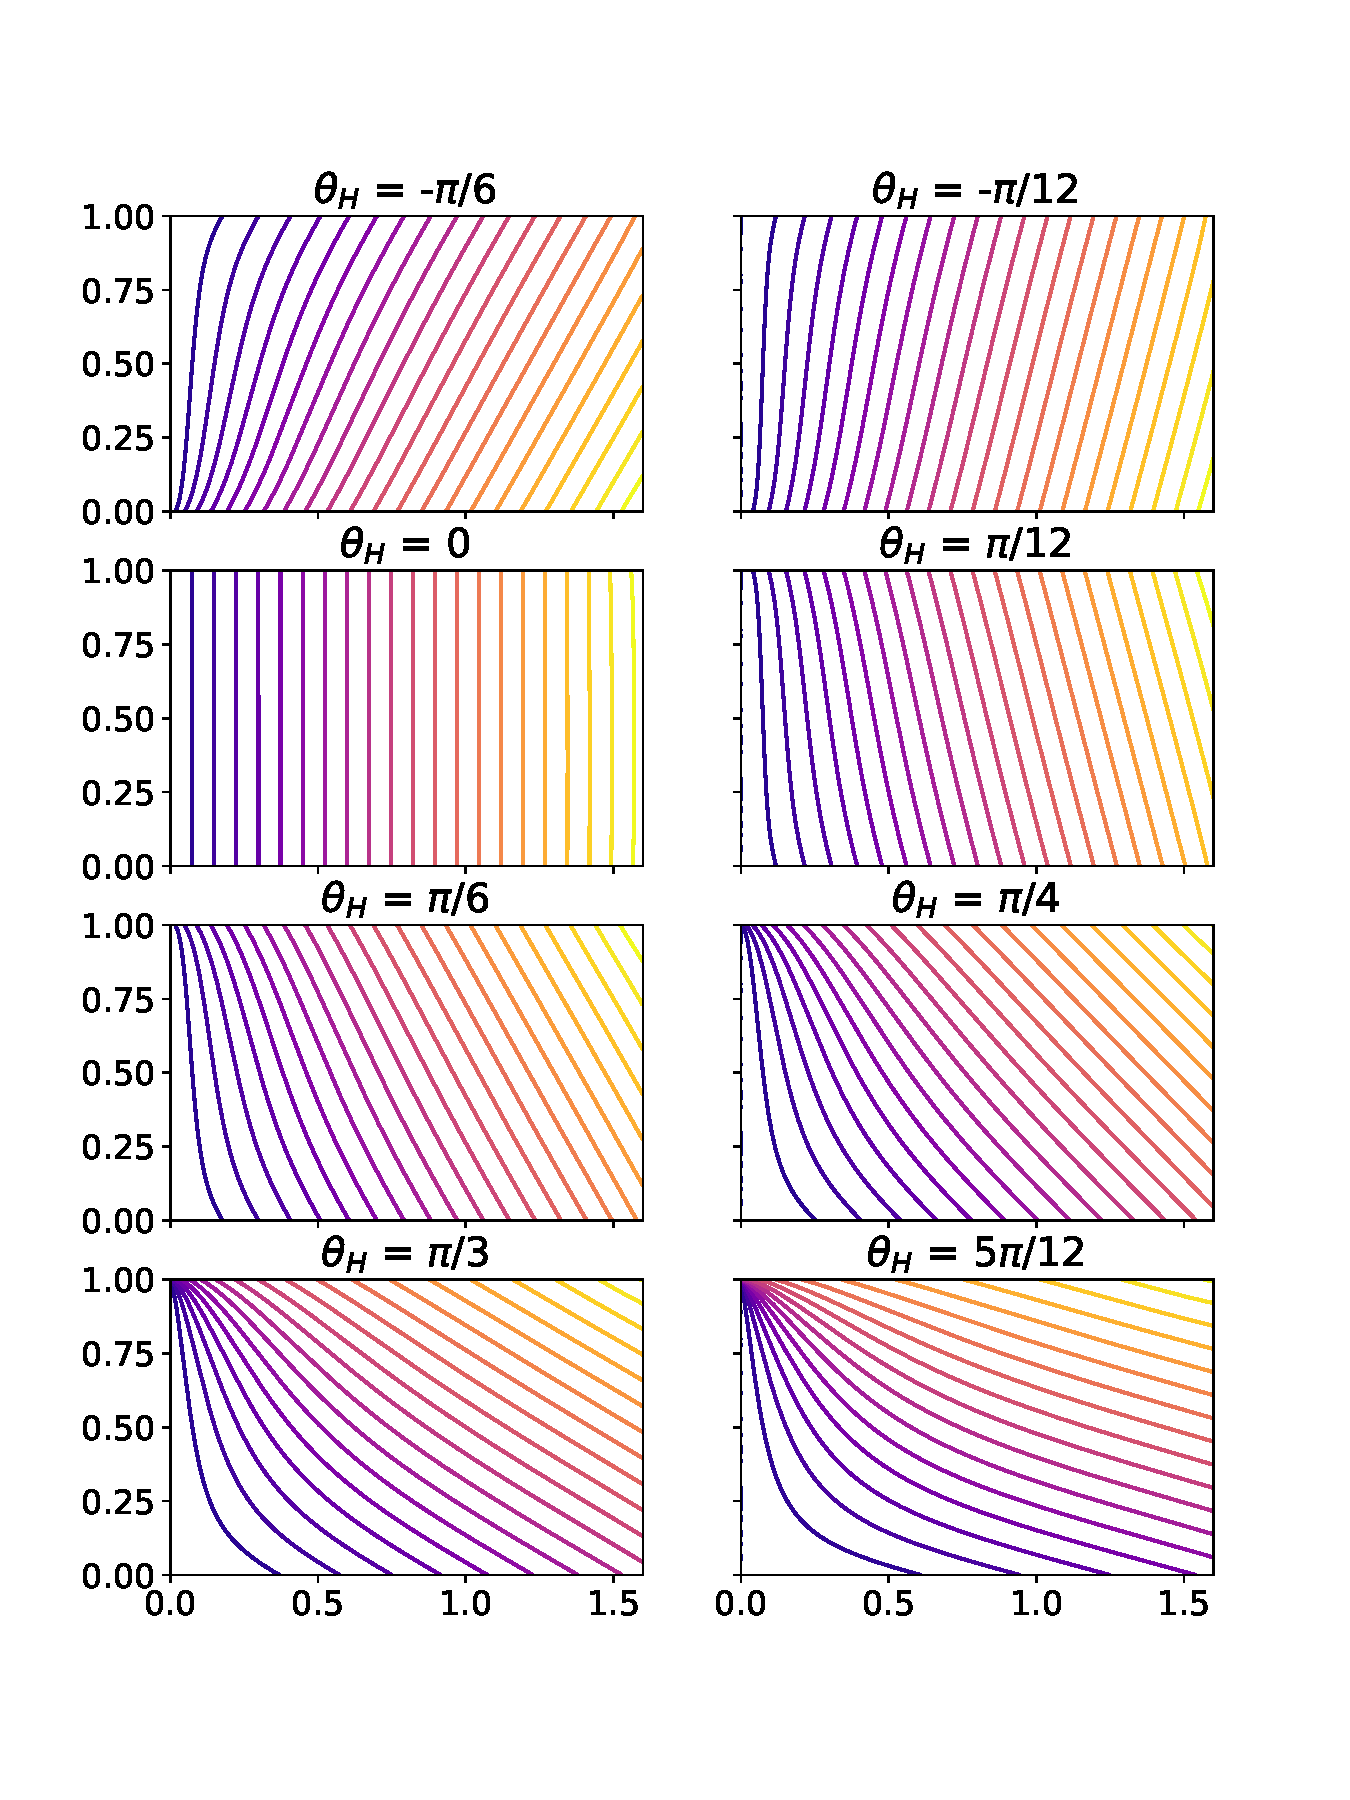
\includegraphics[width=\textwidth]{figures/thall_isotherm.pdf}
\caption[Thermal Hall Isotherms]{Thermal Hall Isotherms. The left side of each simulation is
held to \(T=0\), the right has a heater with unit power, and the upper
and lower edges are insulating.\label{thall_iso}}
\end{figure}

\begin{figure}
\centering
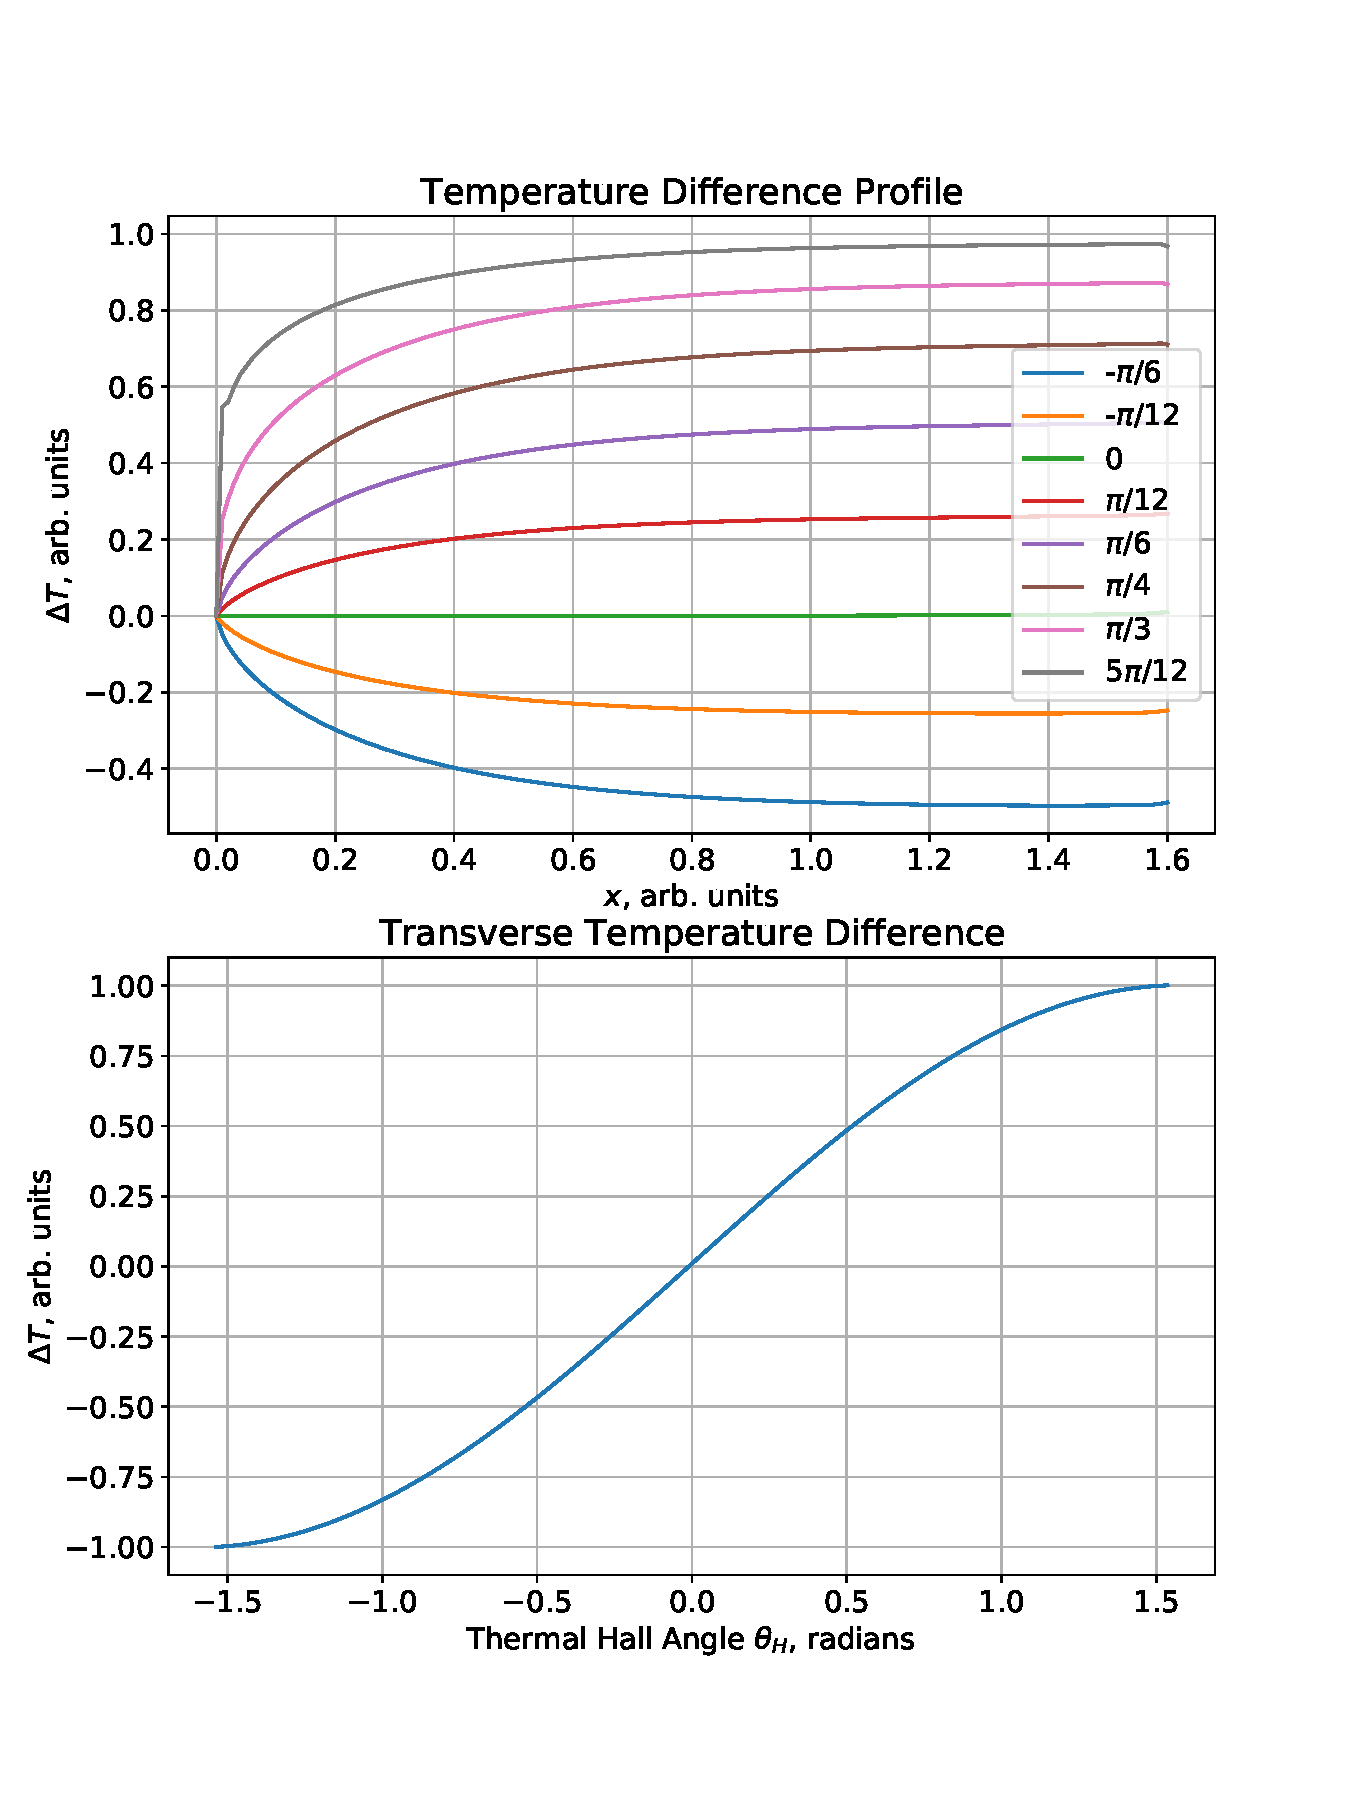
\includegraphics[width=0.9\textwidth]{figures/thall_profile.pdf}
\caption[Thermal Hall Temperature Profiles]{Thermal Hall Temperature Profiles. Top: Temperature difference across
	the sample transverse to the applied heat (y axis in figure
	\ref{thall_iso}) at different points along the sample for different
	thermal Hall angles. Note that for each angle, the temperature
	difference approaches a constant value far from the cold finger.
	Bottom: The same temperature difference at a fixed position as a
function of the thermal Hall angle. Note that for experimentally relevant values of the thermal Hall angle (\(\theta_H \approx 1^\circ\)), \(\Delta T\) is proportional to \(\theta_H\).   \label{thall_prof}}
\end{figure}

This dependence of the Hall signal on the particular boundary condition should
not be suprising to anyone who is experienced making electrical transport
measurements. Indeed, DC electrical transport can be modeled using an analogous
partial differential equation \[ \nabla \cdot (\sigma \nabla V) = 0 \] where
$V$ is the electric potential and $\sigma$ is the conductivity tensor. The
typical geometry for a (non-thermal) Hall effect measurement involves measuring
the voltage at four points on the sample, with the edges of the sample
electically insulating. This gives us the same Neumann boundary condition as
before, via Ohm's law rather than Fourier's law: \[ \hat{n} \cdot \mathbf{j} =
\hat{n} \cdot \sigma \nabla V = 0\] where $\mathbf{i}$ is the current density.
If instead we wish to eliminate the effect of the Hall conductivity, a
different geometry known as a Corbino disk is used~\cite{Eo2018}. This geometry consists of
two large electrodes in the shape of concentric rings, leaving an annular
region where current flows through the sample of interest. In effect, this
clamps the voltage at each point on the two rings (to values which depend on
the applied current and the conductivity of the sample), effectively giving us
a Dirichlet boundary condition (i.e. specifing the voltage) at every point on the boundary. This supresses
the effect of the Hall conductivity, and thus this type of of measurement is
good for isolating the magnetoresistance of a sample.

\begin{figure} \centering
	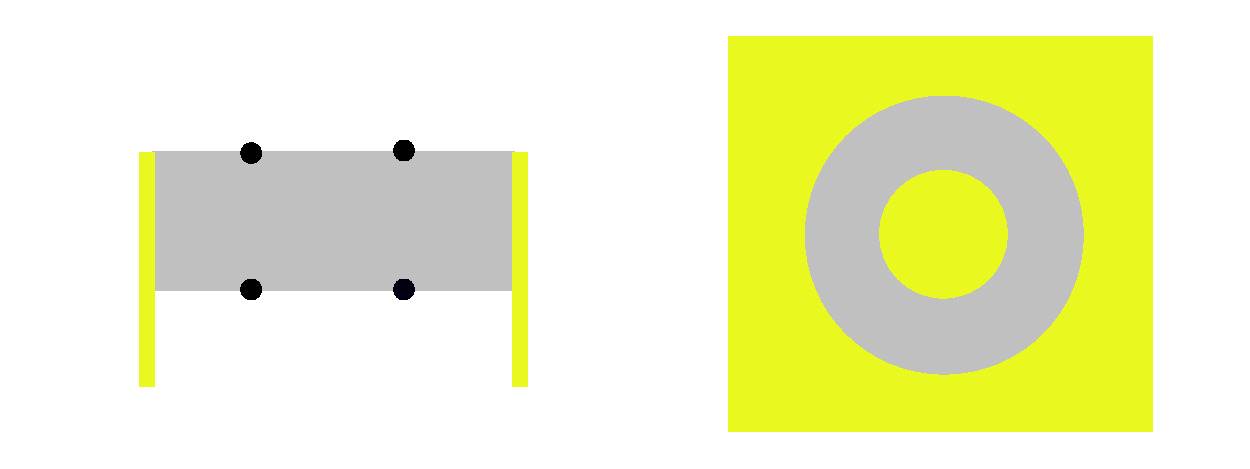
\includegraphics[width=\textwidth]{figures/ehall_geometry.pdf}
	\caption[Electrical Transport Geometries]{Electrical Transport
	Geometries. Left: Hall bar geometry. Current is fed in through the gold
contacts on the left and right, and the voltage measured at the black points.
The upper and lower boundaries are insulating. Right: Corbino disk. The voltage
is measured between the inner and outer contacts (gold). Since there is no
insulating boundary, the Hall conductivity is suppressed.} \end{figure}

This analogy between thermal and electrical transport begs the question: Could
one measure thermal conductivity with a ``thermal Corbino disk''? Maybe, but in
practice it would never be necessary for a very simple reason: in real
materials, the thermal Hall angle is rarely more than a few degrees. Table
\ref{tab:hall_angles} lists a few selected thermal Hall angles reported in the
literature. In all of these materials, the thermal Hall conductivity is the
result of some kind of (quasi-)particle excitation. In the next section, we
will discuss the thermal Hall conductivity of electrons in metals. However, the
last two entries in the table list thermal Hall conductivities which are the
result of excitations which carry spin but not charge. It is this kind of
experiment where measurements of the thermal Hall effect have particular
scientific value, since such quasiparticles cannot be directly observed using
electrical transport methods. Such a measurement will be the subject of chapter
3.

\begin{table}
\centering
\label{tab:hall_angles}
\begin{tabular}{l|r|c}
\hline
Material & $\tan \theta_H$ & Reference \\
\hline
Bi & 0.2 & \cite{Kobayashi2012}  \\
InSb & 0.02 & \cite{Mette1963} \\
HgSe & 0.03 & \cite{Whitsett1961} \\
YBa$_2$Cu$_3$O$_{6.63}$ & 0.12 & \cite{Krishana1999} \\
Lu$_2$V$_2$O$_7$ & $2 \times 10^{-3}$ & \cite{Onose2010} \\
Tb$_2$Ti$_2$O$_7$ & $~5 \times 10^{-3}$ & \cite{Hirschberger2015} \\
\hline
\end{tabular}
\caption[Example thermal Hall angles]{Thermal Hall angles, reported as $\tan \theta_H$, for various materals. Naturally, the specific value is a function of applied field and overall temperature, only the largest reported angle is reproduced here.}
\end{table}
\section{Origin of the Thermal Hall Conductivity in Metals}

The thermal Hall effect in metals has been observed experimental fact for more
than a century. In historical literature, it is known as the Righi-Leduc effect,
named after the Italian and French (respectively) physicists who discovered
it~\cite{Bridgman1924}. In elementary terms, it can be understood as the
correlary of two basic phenomena in solid state physics: the Wiedemann-Franz
law, and the (electronic) Hall effect. The Wiedemann-Franz law refers to the
experimental observation, reproducable in theoretical models such as the
classical Drude model, that the ratio between the thermal and electrical
conductivities of a metal is more or less proportional to the temperature:
\[ \frac{\kappa}{\sigma} = LT, L \approx 2.22 \times 10^{-8}
\textrm{ W}\Omega/\mathrm{K}^2\]
where $L$ is sometimes called the Lorenz constant. Typically $\kappa$ and
$\sigma$ are assumed to be scalars, but within the semiclassical theory of
conduction in metals, we can rigourously derive a relation in terms of the
conductivity tensors while also producing a reasonably accurate value for
$L$. I will summarize the derivation given in chapter 13 of Ashcroft and Mermin
here~\cite{AshcroftMermin}. 

Take for example a region of a solid small enough that we can assume it has
uniform temperature. Assuming that the only thing carrying heat and entropy into
or out of this region is the electrons, we can use the basic thermodynamic
identity in the grand canoncial ensemble ($T dS = dU - \mu dN$, where $U$ is the
total energy, $N$ is the number of electrons, and $\mu$ is the chemical
potential) to express the heat current $\mathbf{j}^q$ in terms of the energy and
number currents ($\mathbf{j}^\mathcal{E}$ and $\mathbf{j}^n$, respectively):
\[ \mathbf{j}^q = T \mathbf{j}^s = \mathbf{j}^\mathcal{E} - \mu \mathbf{j}^n\]
The currents on the right hand side can be expressed in terms of an integral
over the Brillouin zone:
\[ \binom{\mathbf{j}^\mathcal{E}}{\mathbf{j}^n} = \sum_n \int
	\frac{d\mathbf{k}}{4\pi^3}\binom{\mathcal{E}_n(\mathbf{k})}{1}
	\mathbf{v}_n(\mathbf{k})g_n(\mathbf{k}) \]
Where $n$ indexs the bands, $\mathcal{E}_n$ is the band structure,
$\mathbf{v}_n$ is the electron velocity, and $g_n$ is the electron distribution
function. The heat current can be derived in a straightforward way from these
two expressions:
\[ \mathbf{j}^q = \sum_n \int
	\frac{d\mathbf{k}}{4\pi^3}[\mathcal{E}_n(\mathbf{k})-\mu]
	\mathbf{v}_n(\mathbf{k})g_n(\mathbf{k}) \]
Now we consider the modification of $g$ in the case where the a uniform electric
field $\mathbf{E}$, uniform magnetic field $H$, and temperature gradient $-\nabla
T$:
\[ g(\mathbf{k}) = g^0(\mathbf{k}) -
	\tau(\mathcal{E}(\mathbf{k}))\left(-\frac{\partial f}{\partial
		\mathcal{E}}\right)\overline{\mathbf{v}}(\mathbf{k})\left[-e\mathbf{\mathcal{E}}
		+ \frac{\mathcal{E}(\mathbf{k}) - \mu}{T}(-\nabla T)\right] \]
where $f$ is the Fermi-Dirac distribution, $\tau$ is the relaxation time,
\[\mathbf{\mathcal{E}} = \mathbf{E} + \frac{\nabla\mu}{e}\]
and 
\[\overline{\mathbf{v}}_n(\mathbf{k}) = \int_{-\infty}^0
\frac{dt}{\tau_n(\mathbf{k})}e^{t/\tau_n(\mathbf{k}}\mathbf{v}_n(\mathbf{k}(t))\]
is the velocity of the electron averaged over its entire history weighted
exponentially by the relaxation time. This is necessary due to the presence of a
magnetic field, required in order to observe the thermal Hall effect. We will
now use this new distribution function to construct the heat and electrical
currents. The electrical conductivity is given by
\[ \mathbf{\sigma}^{(n)}(\mathcal{E}) = e^2 \int \frac{d\mathbf{k}}{4\pi^3}
\tau_n(\mathcal{E}_n(\mathbf{k}))
\mathbf{v}_n(\mathbf{k})\overline{\mathbf{v}}_n(\mathbf{k})\left(-\frac{\partial
f}{\partial \mathcal{E}}\right)_{\mathcal{E}=\mathcal{E}_n(\mathbf{k})}\]
Define the quantities
\begin{align*} \mathcal{L}^{(\alpha)} &= \int d\mathcal{E} (\mathcal{E} - \mu)^\alpha
\mathbf{\sigma}(\mathcal{E}) \\
	\mathbf{L}^{11} &= \mathcal{L}^{(0)} \\
	\mathbf{L}^{21} &= T \mathbf{L}^{12} = -\frac{1}{e}\mathcal{L}^{(1)} \\
	\mathbf{L}^{22} &= \frac{1}{e^2T} \mathcal{L}^{(2)}
\end{align*}
the current densities can be written straightforwardly as
\begin{align*}
	\mathbf{j} &= \mathbf{L}^{11}\mathbf{\mathcal{E}} +
	\mathbf{L}^{12}(-\nabla T) \\
	\mathbf{j}^q &= \mathbf{L}^{21}\mathbf{\mathcal{E}} +
	\mathbf{L}^{22}(-\nabla T)
\end{align*}
Now, we will use some assumptions valid for metals to make these integrals more
tractable. The derivative of the Fermi distribution $\partial f / \partial
\mathcal{E}$ is only has significant weight in a region centered on the Fermi energy
$\mathcal{E}_F$ with width $k_BT$. Thus, we can use the Sommerfeld expansion to
see that
\begin{align*}
	\mathbf{L}^{11} &= \mathbf{\sigma}(\mathcal{E}_F) = \mathbf{\sigma} \\
	\mathbf{L}^{21} &= T\mathbf{L}^{12} = -\frac{\pi^2}{3e}(k_BT)^2
	\left.\frac{\partial \mathbf{\sigma}}{\partial
		\mathcal{E}}\right|_{\mathcal{E} = \mathcal{E}_F} \\
	\mathbf{L}^{22} &= \frac{\pi^2}{3} \frac{k_B^2T}{e^2}\mathbf{\sigma}
\end{align*}
We can now use these relations to get the thermal conductivity in terms of the
electrical conductivity. First, we impose the condition that the no electic
current is flowing, which implies that \[ \mathbf{\mathcal{E}} = -
(\mathbf{L}^{11})^{-1} \mathbf{L}^{12}(-\nabla T)\]
Plugging this into the equation for the heat current, we get that
\[ \mathbf{j}^q = \mathbf{\kappa}(-\nabla T) \;\mathrm{ where }\; \mathbf{\kappa} = \mathbf{L}^{22} - \mathbf{L}^{21}(\mathbf{L}^{11})^{-1}\mathbf{L}^{12} \]
Using the fact that $\partial \mathbf{\sigma}/\partial \mathcal{E}$ taken at $\mathcal{E} = \mathcal{E}_F$ is of order $\mathbf{\sigma}/\mathcal{E}_F$, we can see that the second term in the above expession is dominated by the first by a factor of $(\mathcal{E}_F/k_B T)^2$, and so to leading order only the first term matters. Thus, from the expression for $\mathbf{L}^{22}$, we can see that 
\[ \mathbf{\kappa} = \frac{\pi^2}{3} \left(\frac{k_B}{e}\right)^2 T \mathbf{\sigma} \]
which is the Wiedemann-Franz law, now cast as a relation between the tensors $\mathbf{\kappa}$ and $\mathbf{\sigma}$, in the presence of a magnetic field. 

This should make some intuitive sense. After all, if the electrons can transmit
heat, they should still do so when their orbits have been modified by the
presense of a magnetic field. It is worth reiterating some of the assumptions
present in this analysis. First of all, we have assumed that we are working
with a metal, where thermal conductivity will be dominated by the electrons. We
should not necessarily expect this behavior to hold for a semiconductor, for
example. One might still expect that even if the Wiedemann-Franz law does not
hold in general for a non-metal, the thermal Hall conductivity should not be
affected by the phonon contribution to the thermal conductivity, as phonons
don't carry spin and so should not couple to a magnetic field. However, there
have been a few observations lately of the thermal Hall effect of phonons,
which has been explained in terms of different materials as an effect of the
Berry curvature of the phonon bands~\cite{Zhang2011} or skew scattering of
phonons off of magnetic impurities~\cite{Mori2014}. Even if we restict to
non-magnetic metals there are examples of deviations from the Wiedemann-Franz
behavior. Potassium, an alkali metal which should in principle have simple
metallic behavior has been observed to have a thermal Hall conductivity which deviates from the Wiedemann-Franz law by
up to 50\% in magnetic fields up to
9T~\cite{Tausch1977}~\cite{Fletcher1978}~\cite{Tausch1979}. While the
Wiedemann-Franz law captures relationship between the Hall effect and the
thermal Hall effect to lowest order, it is important to view it more as a
general empricial guide rather than an iron-clad law. Other effects can become
important in specific materials, even metals.

Measurements of the thermal Hall effect in metals are often not reported as the
thermal Hall angle $\theta_H$, but instead as the thermal Hall coefficent
$R_{\mathrm{TH}}$, defined as \[ R_{\mathrm{TH}} = \frac{1}{B_z}
\frac{dT_y/dy}{dT_x/dx} = \frac{1}{B_z} \frac{\kappa_{xy}}{\kappa_{xx}} =
\frac{\tan \theta_H}{B_z}\] This quantity has units of inverse Teslas, which
suggests that it should be related somehow to mobility. Using the
Wiedemann-Franz law derived above, we can show that it is exactly the Hall
mobility: \[ R_{TH} = \frac{1}{B_z}\frac{\kappa_{xy}}{\kappa_{xx}} =
\frac{1}{B_z}\frac{\sigma_{xy}}{\sigma_{xx}} = \sigma_{xx}R_H = \mu_H\] where
$R_H$ is the standard Hall coefficent. (Parenthetically, it is this relation
which generalizes to the thermal Hall effect in semiconductors:\[R_{TH} \approx
\frac{\kappa_{\mathrm{el}}}{\kappa_{\mathrm{tot}}} \mu_H\] where
$\kappa_{\mathrm{el}}$ and $\kappa_{\mathrm{tot}}$ are the electron/hole and
total thermal conductivities, respectively~\cite{Putley}.) While the caveats involving the applicability of the Wiedemann-Franz law above still apply, we should expect that materials which with high mobilities should also have large thermal Hall coefficents. 

\section{The Thermal Hall Conductivity in Bismuth}

This brings us finally to the specific case of Bismuth. Figure
\ref{fig:bismuth_crystal} shows it's crystal structure. Bismuth is a
semi-metal, by which we mean a material which has both negatively charged
(electrons) and positively charged (holes) carriers. Figure \ref{fig:bismuth_pockets} show how these Fermi pockets are arranged in $k$-space, with one large hole pockets and three smaller electron pockets. It should be noted that
the above analysis of the Wiedemann-Franz law did not make any assumptions
about the charge of the carriers involved, and so it can be applied to the case
of Bismuth. Bismuth is characteristic of semi-metals in that it has a low
carrier density ($4.1 \times 10^{17} /$cm$^3$ for electrons, $3.4 \times
10^{17} /$cm$^3$ for holes~\cite{Jain1962}) and a high mobility (4300 cm$^2$/Vs
for electrons, 1500 cm$^2$/Vs for holes, measured in a thin
film~\cite{Rosenbaum2004}, and as high as 85,600,000 cm$^2$/Vs for electrons
and 37,000,000 cm$^2$/Vs for holes in pure crystals~\cite{Gallo1963}). We
should thus expect that Bismuth should display a large thermal Hall coefficent.

\begin{figure}
	\centering
	\caption[Crystal Strucure of Bismuth]{Crystal Structure of bismuth. One unit cell is displayed along the $c$ axis, and two along the $a$ and $b$ axes. The $c$ axis is denoted the trigonal axis, and the $a$ axis is denoted as the bisectrix. The direction perpendicular to both of these is called the binary axis (this is not the $b$ axis, which forms a 120$^\circ$ angle with the $a$ axis). Image generated with Jmol~\cite{jmol}.}
	\label{fig:bismuth_crystal}
	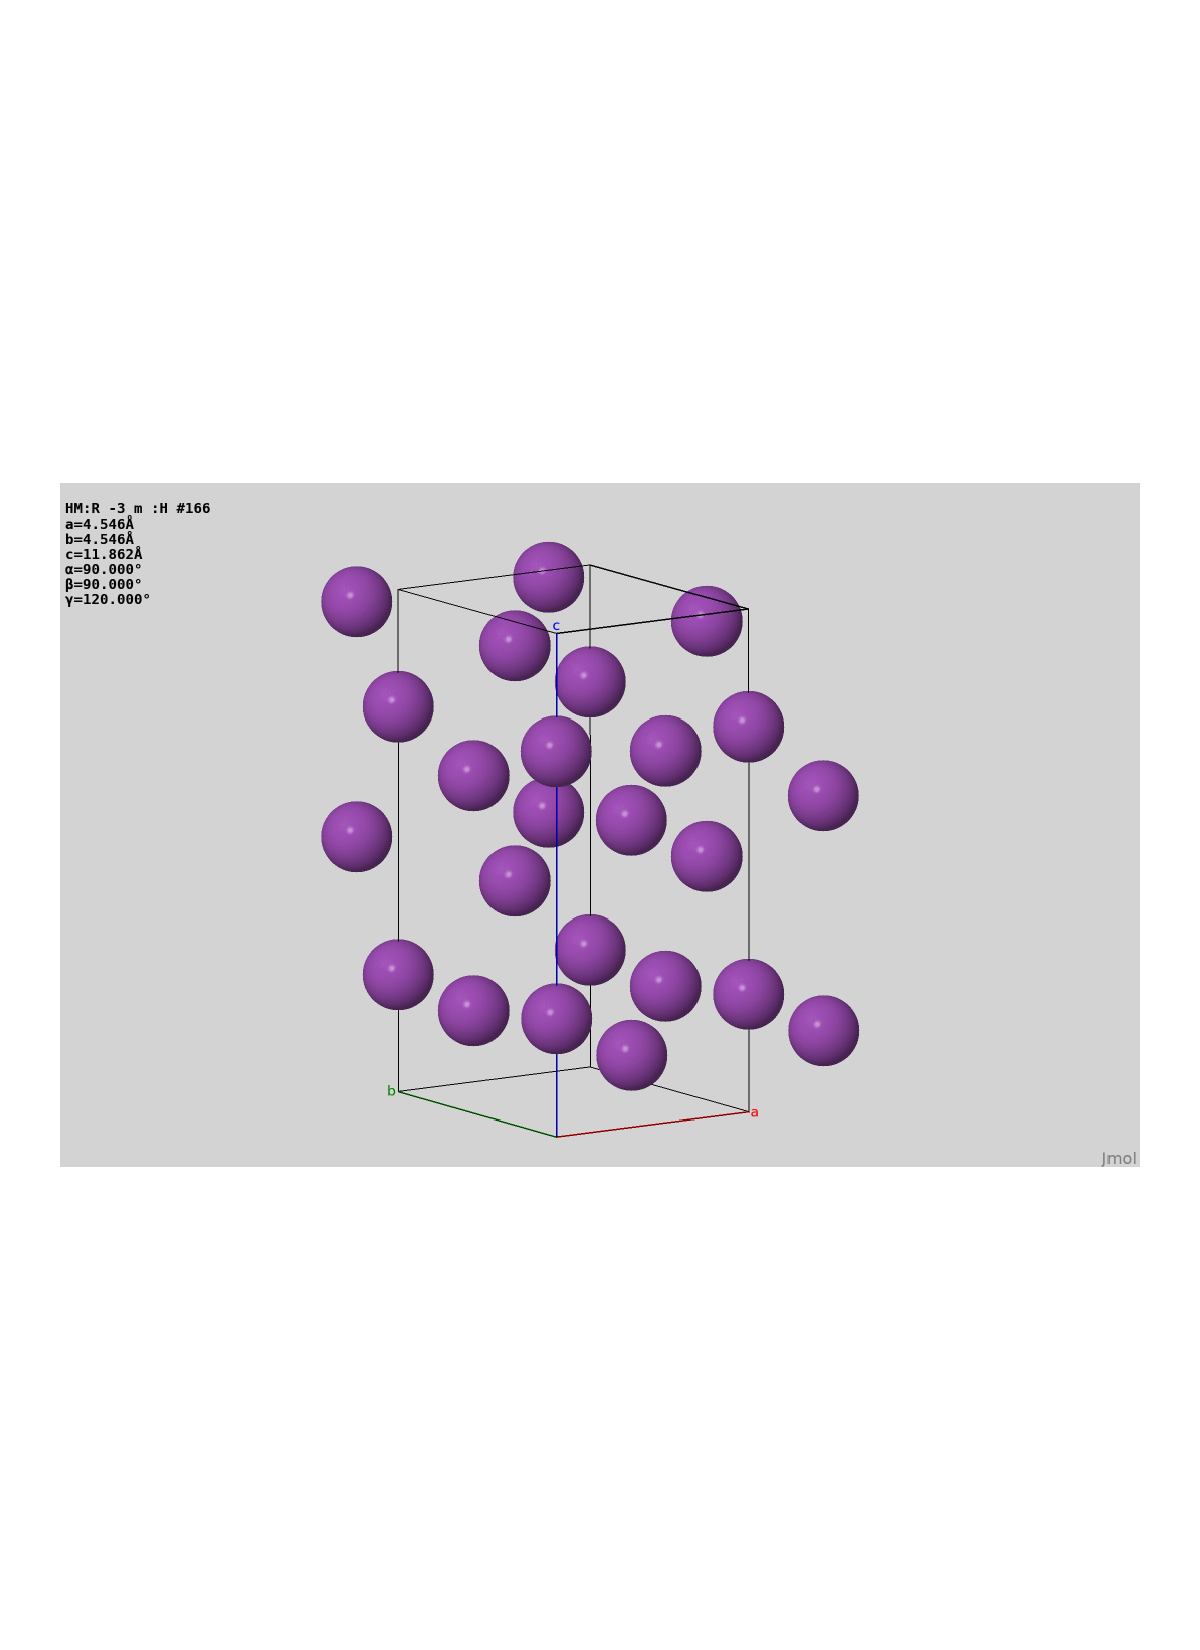
\includegraphics[trim={2in 3in 2in 3in},clip]{figures/bismuth_crystal.pdf}
\end{figure}

\begin{figure}
	\centering
	\caption[Fermi Pockets in Bismuth]{Fermi Pockets in Bismuth. The hole pocket is in ellipsoid with the long axis aligned with the trigonal axis. The three electron pockets are three ellipsoids, one with it's long axis aligned with the bisectrix axis, and the other two distributed 120$^\circ$ either way around the trigonal axis. The electron pockets are canted by 6$^\circ$ degrees out of the bisectrix-binary plane. Image taken from~\cite{Yang2001}.}
	\label{fig:bismuth_pockets}
	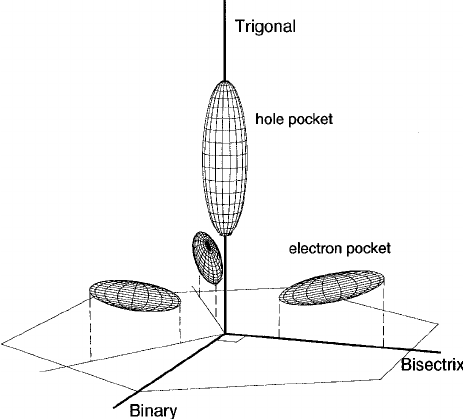
\includegraphics[width=0.5\columnwidth]{figures/bismuth_pockets.png}
\end{figure}

It is worth thinking about how the presence of two carriers will affect the Hall coefficent, as it will have direct consequences for the thermal Hall coefficent. In a simple model, we can imagine that the two carriers act as two seperate conductive channels in parallel with each other. The channels each have resistivity tensors of the form
\[ \mathbf{\rho_e} = \begin{pmatrix}
		\rho_e & -R_eH \\
	R_eH & \rho_e \end{pmatrix} \quad
   \mathbf{\rho_h} = \begin{pmatrix}
   		\rho_h & -R_hH \\
	R_hH & \rho_h \end{pmatrix}\]
where $\rho$ is the longitudinal resistivity of the channel, $R$ is it's Hall coefficent, and $H$ is the applied magnetic field. Note that since the electrons and holes have differing sign, so do $R_e$ and $R_h$. Since these channels are in parallel with each other, the total resistivity is given by 
\[ \mathbf{\rho} = \left(\mathbf{\rho_e}^{-1} + \mathbf{\rho_h}^{-1}\right)^{-1} \]
This results in a total resistivity tensor given by
\[ \mathbf{\rho} = \begin{pmatrix}
		\rho & -RH \\
		RH & \rho \end{pmatrix} \]
where
\[ \rho = \frac{\rho_e \rho_h(\rho_e + \rho_h) + (\rho_e R_h^2 + \rho_h R_e^2)H^2}{(\rho_e + \rho_h)^2 + (R_e + R_h)^2H^2}\]
\[ R = \frac{R_e \rho_h^2 + R_h \rho_e^2 + R_e R_h (R_e + R_h)H^2}{(\rho_e + \rho_h)^2 + (R_e + R_h)^2 H^2} \]
Both the longitudinal resistivity and Hall coefficent depend explicitly on the applied field $H$, unless $R_e = -R_h$. Since the Hall coefficent is inversely proportional to the carrier density, and and bismuth has different densities for electrons and holes (see above), we can see that this is not the case for bismuth. In practice, this means the resistivity and Hall coefficent basically have two regimes, a low field regime where
\[ \rho = \frac{\rho_e \rho_h}{(\rho_e + \rho_h)} \quad R = \frac{R_e \rho_h^2 + R_h \rho_e^2}{(\rho_e + \rho_h)^2} \]
and a high field regime where
\[ \rho = \frac{\rho_e R_h^2 + \rho_h R_e^2}{(R_e + R_h)^2} \quad R = \frac{R_e R_h}{R_e + R_h} \]
Figure \ref{fig:bismuth_hall} is a plot of experimental datat which shows this behavior: two linear regimes, one at high field, and one at low field.

\begin{figure}
	\caption[Hall conductivity in bismuth]{Hall conductivity in bismuth, measured at 10K in our Janis cryostat. Notice the two linear regimes, one at low field and one at high field, consistent with the two carrier model.}
	\label{fig:bismuth_hall}
	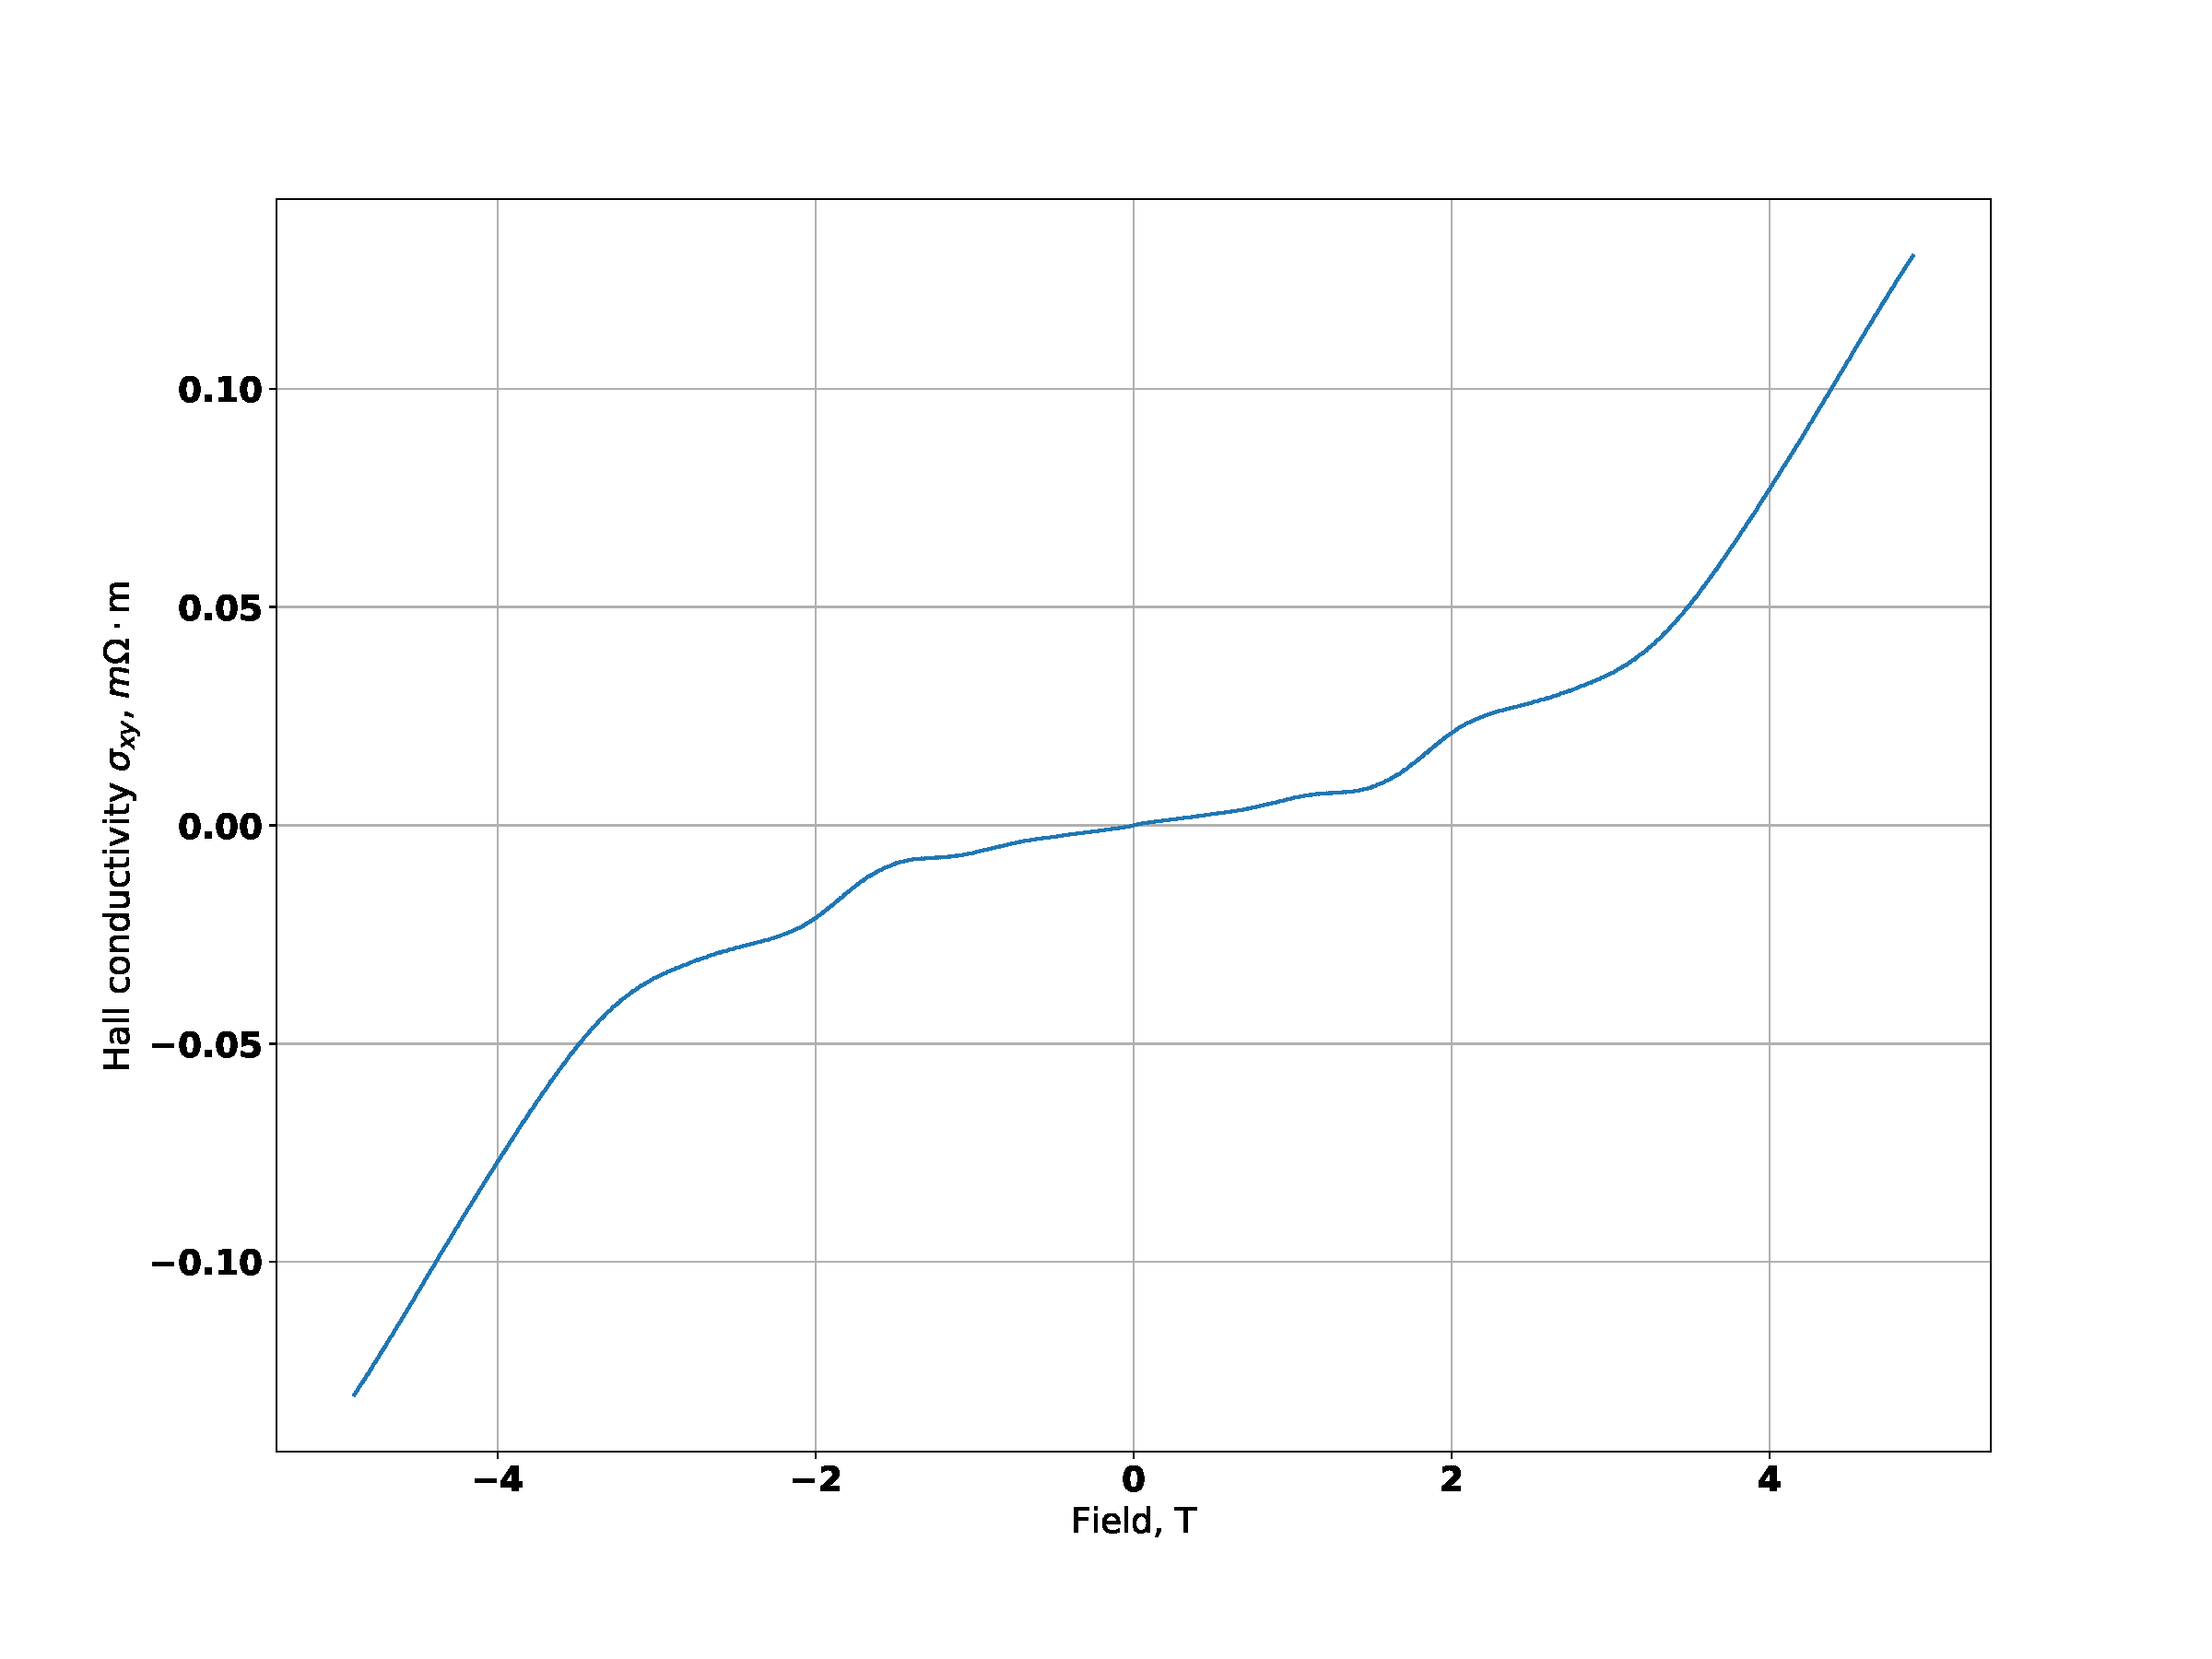
\includegraphics[width=\columnwidth]{figures/BiHallEffect.pdf}
\end{figure}

What does this imply for the thermal Hall conductivity? Well, from the Wiedemann-Franz law, we can see that the thermal Hall coefficent is given by
\[ R_{\mathrm{TH}} = \sigma R_{\mathrm{H}} = \frac{R}{\rho}\]
as shown above. Rearranging terms and appling the Wiedemann-Franz law again, we get:
\[ R_{\mathrm{TH}} = \frac{1}{H}\frac{\kappa_{xy}}{\kappa_{xx}} = \frac{1}{H}\frac{\kappa_{xy}}{LT\sigma}\]
\[ \Rightarrow \kappa_{xy} = \frac{R}{\rho^2}HLT \]
where $L$ is the Wiedemann-Franz constant and $T$ is the temperature. Thus $\kappa_{xy}$ will be a function of the applied magnetic field $H$ just as $R$ and $\rho$ are. If we take the low and high field regimes, however, $\kappa_{xy}$ should be more or less linear with field. Taking the low field expression for $R$ and $\rho$ gives us
\[ \kappa_{xy,\mathrm{LOW}} = \frac{R_e\rho_h^2 + R_h \rho_e^2}{\rho_e^2 \rho_h^2} HLT \]
So for small fields, $\kappa_{xy}$ should be linear in the applied field. In the high-field limit, the expression becomes
\[ \kappa_{xy,\mathrm{HIGH}} = \frac{R_e R_h (R_e + R_h)^3}{(\rho_e R_h^2 + \rho_h R_e^2)^2} HLT \]
At first glance, this looks qualitatively similar to the low field expression, linearly proportional to the applied field. However, remember that $R_e$ and $R_h$ have different signs, but are of the same order of magnitude. This implies that their sum should be small. In this expression, we take that small sum and cube it, making it even smaller. In the denominator, we take a linear combination of the squares of $R_e$ and $R_h$ (which are both positive now) and square them again. This indicates, at least qualitatively, that the high field coefficent should be much smaller than the low field coefficent.


\begin{figure}
	\centering
	\begin{minipage}{.45\linewidth}
	\caption[Thermal Hall conductivity in Bismuth up to 3 T]{Thermal Hall conductivity in Bismuth, measured up to 3 T measured by \cite{Kobayashi2012}. Note that in all the traces down to 75K, the low field dependence is linear, and in the lower temperature curves we can see the high field thermal Hall conductivity go to zero.}
	\label{fig:kobayashi1}
	\includegraphics[width=\linewidth]{figures/kobayashi12_fig1.pdf}
	\end{minipage}
	\hspace{.05\linewidth}
	\begin{minipage}{.45\linewidth}
		\caption[Temperature dependence of $R_{TH}$ in bismuth up to 3 T]{Temperature dependence of the thermal Hall coefficent in bismuth up to 3 T and 300K, taken from \cite{Kobayashi2012}. The dependence is not strictly linear with temperature, and follows more or less the temperature dependence of the Hall mobility $\mu_H$.}
	\label{fig:kobayashi2}
	\includegraphics[width=\linewidth]{figures/kobayashi12_fig2.pdf}
	\end{minipage}
\end{figure}

How well do these predictions bear out in practice? Suprisingly, measurements of the thermal Hall effect in bismuth have only been carried out in high magnetic fields relatively recently, by Kobayashi et al. in 2012~\cite{Kobayashi2012}. In that work, measurements of the thermal Hall coefficent were performed in fields up to 3T and temperatures from room temperature down to 75K. Figure \ref{fig:kobayashi1} reproduces their results in measuring the transverse temperature gradient. We can see that for all the traces, the low field dependence is linear, with the slope decreasing at higher field. In some of the lower temperature traces, we can also see the thermal Hall conductivity tend towards zero at higher field. This would seem to reproduce the qualitative features discussed above. Additionally, figure \ref{fig:kobayashi2} from the same paper show the temperature dependence of the thermal Hall coefficent $R_{\mathrm{TH}}$. Although I did not remark on it above, the basic analysis would indicate that the thermal Hall coefficient should increase linear in temperature. The experimental data shows this is clearly not the case. Instead, the data shows that the thermal Hall coefficent generally follows the temperature dependence of the Hall mobility $\mu_H$. This is not suprising, as they should be directly related.

One possible objection to the prediction that the thermal Hall coefficient should be effectively zero at high field might be that since it is not exactly zero, with a sufficently large field one should be able to see a non-zero thermal Hall conductivity once again. This presupposes that the simple two-carrier model described above is applicable for arbitrarily large applied fields. The validity of this assumption is contradicted by the physics of Landau quantization in metals, i.e. the quantization of the circular path of a charged particle in a magnetic field. This effect is responsible for the oscillations seen in many observables (such as resistivity and magnetic susceptibility) in strong magnetic fields~\cite{Shoenberg}. As the field gets stronger, the Landau levels get farther apart in energy and more degenerate, until all the carriers are collected in the lowest level. This is known as the quantum limit. This has the effect of gapping out the carriers, and so we would expect that they would no longer participate in the thermal Hall effect. The field at which this happens is proportional to the cross-sectional area of the Fermi surface perpendicular to the applied field~\cite{Shoenberg}, and since bismuth has small Fermi pockets we should expect this to happen at relatively low fields. The field at which this happens depends strongly on the angle due to the elongated fermi pockets, but is less than 8T for all angles~\cite{Li2008}. This will ultimately supress the thermal Hall coefficent at these fields. Making measurements of the thermal Hall effect at these fields presents some experiemental challenges, however. Before we can discuss those difficulties, we must discuss the experimental setup for making any thermal Hall effect measurement.  


\section{Performing Thermal Hall Effect Measurements}
Now that we have discussed the origin of the thermal Hall effect in metals, we
must now discuss how one makes the measurement. Figure~\ref{fig:thall_geometry}
shows a schematic of the measurement. The sample is attached to a cold finger,
typically by way of a thermally conductive sample holder (made of oxygen-free
copper, in our case). This controls the overall temperature of the sample. On the other end of the sample, a small resistive heater is attached using thermally conductive paste. This setup mirrors the boundary conditions of the finite element calculations presented above: one side (the cold finger) is held at a fixed temperature, the opposite (the heater) has a prescribed amount of heat energy applied, and the two perpendicular boundaries are (ideally) assumed to be insulating. Experimentally, this means performing the measurment in vacuum.

\begin{figure}
	\caption[Schematic of a thermal Hall effect measurement]{Schematic of a thermal Hall effect measurement. The magnetic field is applied out of the plane of the page. Both the longitudinal ($\Delta T_x$) and transverse ($\Delta T_y$) temperature gradients are measured. If nessicary, the measurement can be carried out with two thermometers, and the gradients disentangled by (anti-)symmetrizing the measured gradient with respect to the applied field.}
	\label{fig:thall_geometry}
	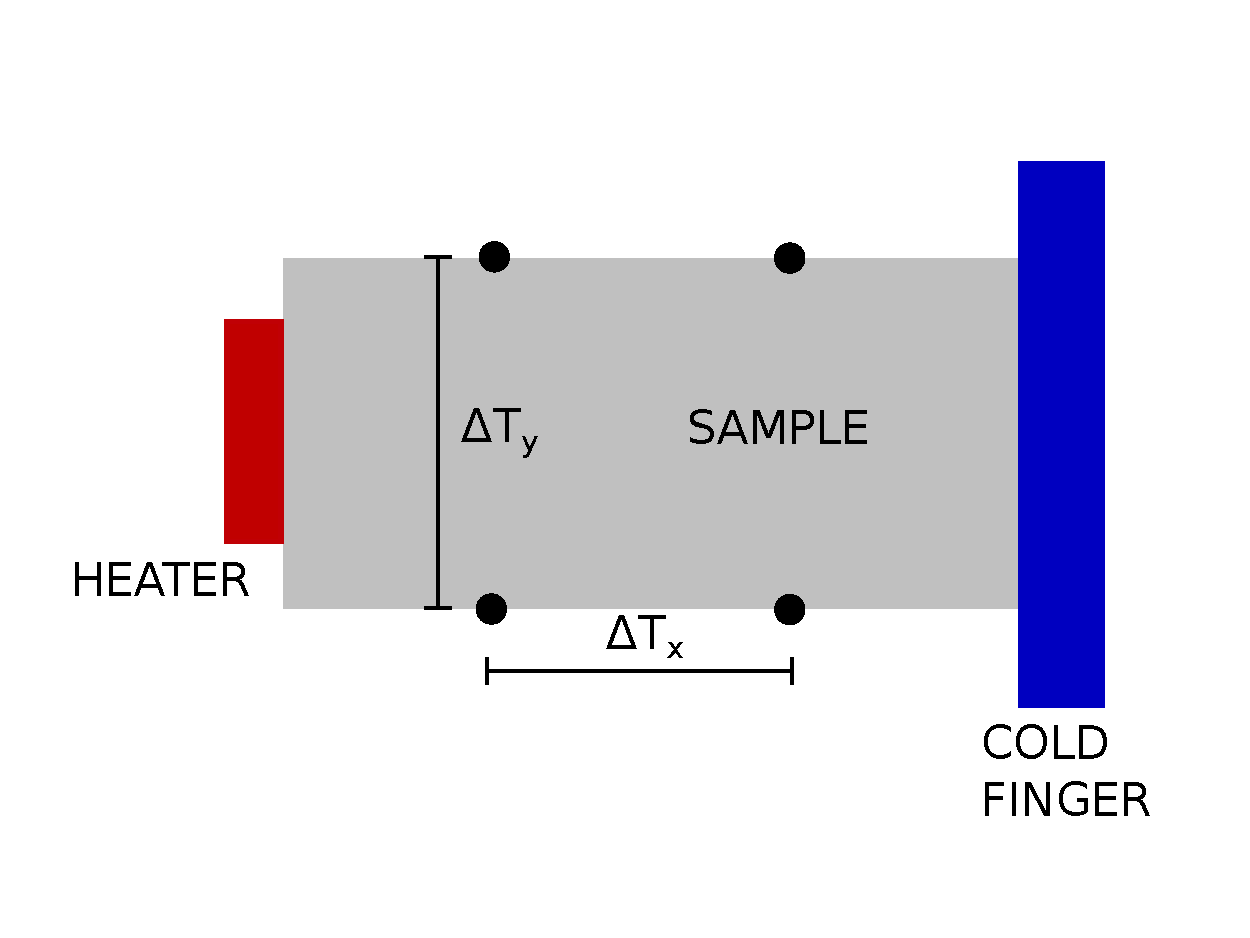
\includegraphics[width=\columnwidth]{figures/thall_geometry.pdf}
\end{figure}
In order to measure the thermal Hall conductivity, we should ideally place three thermometers on the edge of the sample. This allows us to measure two temperature gradients: the longitudinal (along the direction pointing from the heater to the cold finger, denoted $\Delta T_x$) and the transverse (perpindicular to the longitudinal gradient, denoted $\Delta T_y$). If the thermometers are small enough relative to the sample, they can be mounted directly to the sample with a thermally conductive paste, similar to the heater. Alternatively, the thermometers can be mounted seperately and thermally linked to the sample with gold wire. We can use this information along with the applied power $P$ to determine the terms of the thermal conductivity tensor by writing Fourier's law as
\[ \begin{pmatrix}
		j_x \\
		j_y \\
\end{pmatrix}
= \begin{pmatrix}
	-P/(t\cdot w) \\
	0
\end{pmatrix}
= \begin{pmatrix}
	\kappa_{xx} & \kappa_{xy} \\
	-\kappa_{xy} & \kappa_{yy} 
\end{pmatrix}
\begin{pmatrix}
	-\Delta T_x/l \\
	-\Delta T_y/w
\end{pmatrix} \]
where $l$ is the length between the two longitudinal thermometers, $t$ is the thickness of the sample, and $w$ is the width of the sample (i.e. $t\cdot w$ is the cross sectional area of the sample perpindicular to its length). The assumption that $\kappa_{yx} = - \kappa_{xy}$ is taken from a relation due to Onsager (note that these are not the Onsager reciprocal relations of statistical mechanics, for details on where this relation comes from see problem 6f of chapter 13 of Ascroft and Mermin~\cite{AshcroftMermin}). If we further assume that the heat conduction is isotropic, that is $\kappa_{xx} = \kappa_{yy}$, we are left with two equations in two unknowns, $\kappa_{xx}$ and $\kappa_{xy}$:
\begin{align*}
		P / (t \cdot w) &=  \kappa_{xx} \Delta T_x / l + \kappa_{xy} \Delta T_y / w \\
		0 &= \kappa_{xy} \Delta T_x / l - \kappa_{xx} \Delta T_y /w 
	\end{align*}
The second line gives the relation
\[ \kappa_{xy} \Delta T_x w = \kappa_{xy} \Delta T_y l \Rightarrow \kappa_{xy} = \kappa_{xx} \frac{\Delta T_y l}{\Delta T_x w} \]
substituting this result into the first equation gives
\[ P \cdot l = \kappa_{xx} \left( \Delta T_x w t - \frac{\Delta T_y^2 l^2 t}{\Delta T_x w} \right) \approx \kappa_{xx} \Delta T_x w t\]
For the last step, we are making use of the fact that the thermal Hall angle is generally small, so $\Delta T_x$ is much larger than $\Delta T_y$. Now we can use these relations to get the terms of the conductivity tensor in terms of known variables:
\[\kappa_{xx} = \frac{P l}{\Delta T_x wt} \quad \kappa_{xy} = \frac{P \Delta T_y l^2}{\Delta T_x^2 w^2t} \]
These are the relations use to determine the thermal Hall conductivities in the experiments described in the coming chapters.

As stated above, ideally one would use at least three thermometers to measure the transverse and longitudinal thermal gradients. However, each thermometer allows a small amount of heat to escape the sample, which contradicts the ideal case where the boundary is perfectly insulating. We can minimize the amount of heat lost this way by only using two thermometers, with an offset in both the $x$ and $y$ directions. This poses the problem of how the $\Delta T_x$ and $\Delta T_y$ can be disambiguated. In the case of a thermal Hall effect measurement taken at a constant temperature in a sweeping magnetic field, the Onsager transport relation mentioned above implies that the $\kappa_{xx}$ and $\kappa_{xy}$ have different symmetry with respect to the field:
\[ \kappa_{xx}(H) = \kappa_{xx}(-H) \quad \kappa_{xy}(H) = -\kappa_{xy}(-H) \]
By inspection we can see that this implies that $\Delta T_x(H)$ is even in $H$, and $\Delta T_y(H)$ is odd. Thus, the two temperature gradients can be disambiguated by taking the measurment by performing the measurement in both positive and negative field, and extracting the proper gradients by (anti-)symmetrizing the gradient measured between the two thermometers.

\begin{figure}
	\caption[Raw temperature gradient data]{Raw temperature gradient data, in this case a longitudinal temperature gradient measured using a pair of thermocouples on a bismuth sample. The raw data is in blue, and the extracted enveloples are in red and green.}
	\label{fig:raw_data}
	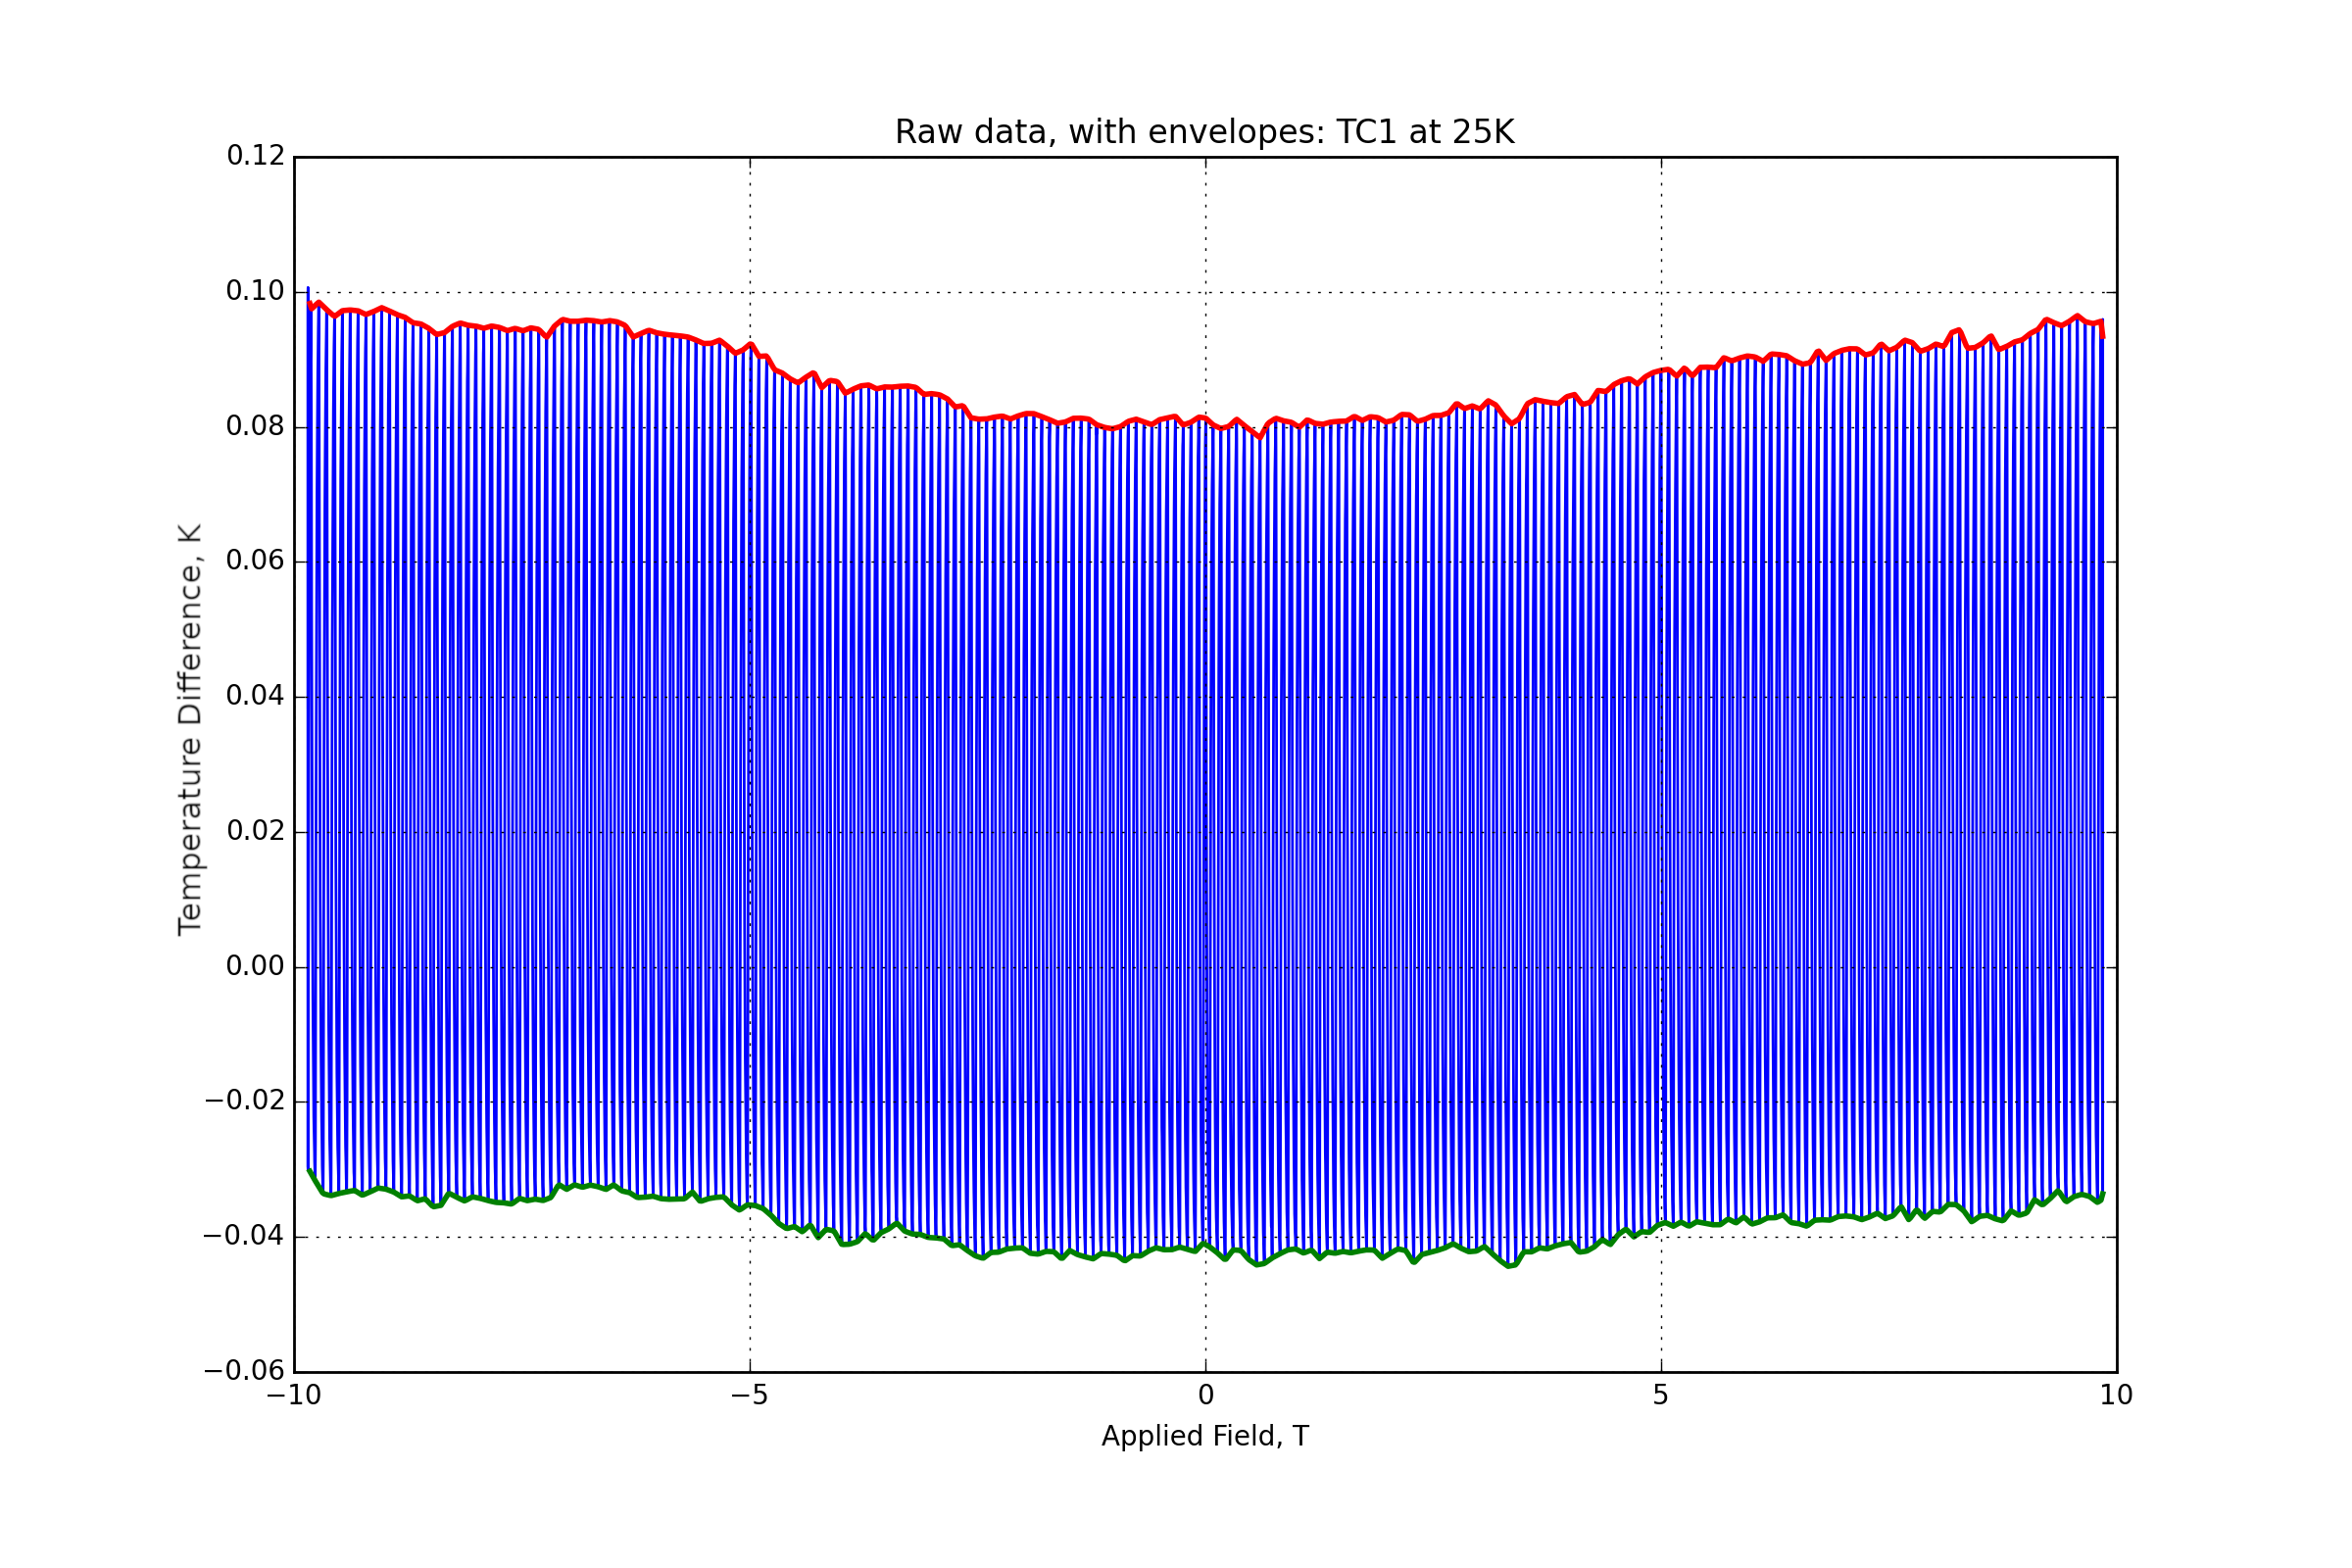
\includegraphics[width=\columnwidth]{figures/25K_TC1_Raw.png}
\end{figure}

Based on the previous discussion, one might think that the best way to conduct a thermal conductivity measurement would be to simply run the heater with a constant power and measure the thermal gradients as a function of the relevant experiemental variable (e.g. magnetic field for a thermal Hall effect measurement). However, if the overall temperature of the sample were to drift, or if there is any temperature gradient in the smaple when there is no heat applied, this will appear as a suprious signal in the thermal conductivities. This can be corrected by pulsing the heater on and off over the course of the measurement rather than keeping it constant. In many cases, a square wave is used: the heater is turned on for some time, and then turned off for some time. The period must be long enough that the sample reaches equalibrium during each on-cycle and off-cycle. This allows the overall background drift to be subtracted away from the measurement. This method is certianly viable, but my preference is to use a sine wave excitation on the heater instead. This has the advantage of never bringing the sample out of equalibrium as long as a low enough frequency is chosen. If we denote the current through the heater as $i(t) = i_0 \sin \omega t$, the power coming out of the heater will be
\[P(t) = I^2R = i_0^2R \sin^2 \omega t = i_0^2 R \frac{1 - cos(2\omega t)}{2} \]
i. e. it will have twice the frequency of the excitation current. The temperature of each thermometer, or alternatively the difference in temperature between any pair of thermometers, will have the general form
\[ T_n(t) = A(t)\sin^2 \omega t + D(t) \]
where $A(t)$ is the difference between the temperature with the heater on and with the heater off, and $D(t)$ is the overall drift. There are two conditions to ensure that $\omega$ is sufficiently small: $A$ should not change with $\omega$, and $P(t)$ should have the same phase as $T_n(t)$. The problem of finding the temperature gradients thus rests on extracting $A(t)$. This amounts to the problem of demodulating an AM signal.

One simple method for accomplishing this is by simply using a peak detection function. Figure \ref{fig:raw_data} shows some raw temperature gradient data from the experiements on bismuth which will be described later in this work. The blue curve shows the raw data, still mixed with the ``carrier''. One attactive feature of the sine wave exicitation is it produces well defined peaks suited for automatic peak detection. Taking the maxima and minima, we can interpolate between them to get the upper and lower envelopes $E_{\mathrm{upper}}(t)$ and $E_{\mathrm{lower}}$. The amplitude and drift can be expressed straightforwardly as
\[ A(t) = E_{\mathrm{upper}}(t) - E_{\mathrm{lower}}(t) \quad D(t) = \frac{E_{\mathrm{upper}}(t) - E_{\mathrm{lower}}(t)}{2} \]
This method is simple to implement, and has the advantage that we do not need any phase information from the heater excitation to determine the gradients. It does however require that we are able to unambiguously detect the peaks.

There is another method which exploits the similarity of this problem to that of demodulating an AM radio signal, known as a ``product detector''. First, we expand the raw signal using the double angle identity:
\[T_n(t) = A(t) \sin^2 \omega t + D(t) = A(t) \frac{1 - \cos 2 \omega t}{2} + D(t)\]
As long as $A(t)$ and $D(t)$ are varing slowly compared to the ``carrier frequency'' $2\omega$, we can use a high pass filter to isolate the $\cos 2\omega t$ term, leaving us with
\[T_n(t) = \frac{A(t)}{2}\cos 2\omega t\]
Next, we multiply this by $\cos 2 \omega t$. This requires us to have proper phase information about the excitation current. Doing this gives
\[ \frac{A(t)}{2} \cos 2 \omega t \cos 2 \omega t = \frac{A(t)}{2}\left(\frac{1}{2} + \frac{1}{2} \cos 4 \omega t \right) \]
Now, once we low pass filter this signal, we end up with $A(t)/4$. There are variations of this method which involve multipling by a higher order power of the ``carrier'' which result in a higher frequency signal which needs to be filtered away. This method does need us to preserve phase information about the excitation current, but does not require any peak detection.

There is one significant experimental detail which has been elided over in this analysis: What kind of thermometers can be used, and what advantages and disadvantages these have. This is not a trivial detail: to make thermal Hall effect measurements, we require thermometers which are both sensitive to millikelvin temperature gradients while not being affected by a magnetic field. We have found that commercially available thermometers have not been able to keep up with our requirements in this respect. In the next chapter, I will describe the research project I undertook to develop thermometers which better satisfied these requirements, as well as the thermal Hall effect measurements on bismuth I made to benchmark these new thermometers.

\chapter{Strontium Titanate Microthermometers}


\section{Thermometry}

Temperature, in its most general form, is a consequence of the ``zeroth'' law
of thermodynamics: If two bodies A and B are in thermodynamic equalibrium, and
B is in thermodynamic equalibrium with a third body C, then A and C are in
thermodynamic equalibrium with each other as well. Thus, the quality of being
in thermodynamic equalibrium is an equivalance relation, and we can define a
temperature scale by assigning a numerical value to each of its equivalence
classes. If we take care to assign this quantity such that one with a higher
temperature will transfer heat to one with a lower temperature when they are
brought in contact (a corollary of the second law of thermodynamics) as well as
the existence of an absolute lowest temperature (the third law), we will arrive
at an experimentally useful temperature scale. Within the formalism of
statistical mechanics, we can construct  such a temperature scale within the
microcanonical ensemble as function of the total energy \(E\) and information
about the states of the system: \[\frac{1}{T} = \frac{dS}{dE} = \frac{d}{dE} k
\log W\] where \(W(E)dE\) is the number of states with energy between \(E\) and
\(E+dE\) and \(k\) is Boltzmann's constant. This function, however, can only be
computed explicity for the simplest physical systems. In practice, if we want
to study the flow of heat through a system by measuring temperature, we must
find some other observable we can measure as a proxy.

In principle, we might want to find some system whose thermodynamic
equation of state depends on temperature and other quantities which are
all independant of temperature. Such a system is refered to as a primary
thermometer. For a simple example of such a thermometer, consider the
equation of state of an ideal gas: \[PV = NkT\] If we take a sample of
an ideal gas with a known number of molecules \(N\) in a known volume
\(V\), we can determine the temperature \(T\) by measuring its pressure
\(P\). Other examples of primary thermometers include measurements of
the speed of sound in a gas, measurements of the Johnson-Nyquist noise
in an electrical circuit, or measurements of blackbody radiation
\cite{Ekin2006}. These methods of measuring temperature are very useful
for accurately setting a temperature scale, but they have some serious
drawbacks as thermometers for use in other experiments. Most of them
require sensitive measurements of multiple physical observables, as well
as bulky and complicated experimental apparatus. If one wanted to
determine the thermal conductivity of a small crystal by measuring a
temperature gradient across its length, it would not be feasable to
connect the crystal to two independant samples of an ideal gas and
measure their pressures. Thus, the temperature standard set by these
methods must be transferred to a more convenient thermometer.

Such a device is known as a secondary thermometer. In this case, we
measure some observable as a function of temperature, which we determine
from some known standard. This can be a primary thermometer or another
secondary thermometer which has already been calibrated to sufficient
accuracy. In experimental condensed matter physics, by far the most
common types of secondary thermometers used are resistance thermometers
and thermocouples. Resistance thermometers simply measure the resistance
of some material as a proxy for temperature, either a metal such as
platinum (resistance increasing with higher temperature, or ``positive
temperature coefficent'') or a semiconductor, such as
zirconium--oxynitride (known by its trademarked name Cernox) or
ruthenium oxide (resistance decreasing with higher temperature, or
``negative temperature coefficent''). Such thermometers are convenient
since they can be made compact, they are commercially available, and
there are well--established protocols and instrumentation for measuring
resistance. There are a wide variety of resistance thermometers that
suit different temperature ranges and experimental conditions.
Thermocouples, which measure the temperature dependant thermopower
between two metals with differing carrier concentrations, can be even
more compact and are especially useful for making differential
measurements. However, they require measurments of DC voltages in the
microvolt range, and their sensitivy is reduced at low temperature. In
any case, both of these methods allow us to measure temperature without
considering the microscopic details of the system, only how accurately
it has been calibrated.

There are some experimental details which must be considered when using a
resistance thermometer. Many important experimental techniques in condensed
matter physics involve applying an intense magnetic field (up to 45T for the
current state-of-the-art DC magnets) to a sample of interest. Resistance
thermometers generally exhibit magnetoresistance, the changing of their
resistivity in a magnetic field. The most commonly used resistance thermometers
are selected to have as small a magnetoresistnace as possible, but even Cernox
thermometers display a change of resistance of a few percent in magnetic fields
up to 14T. If one is not measuring any direct thermal property of a sample and
can safely assume that the sample is well thermalized with the cold finger, one
can simply mount a thermometer outside the region of intense magnetic field.
However, if you are measuring some thermal propety of a material (such as heat
capacity or thermal conductivity), there is no getting around calibrating the
thermometer as a function of temperature and magnetic field (see figure
\ref{cernox_fieldcal}). For resistive thermometers such as Cernox or Ruthenium
Oxide, the magnetoresistance can vary quite a bit from thermometer to
thermometer, as they can have slightly different doping levels. Additionally,
Cernox thermometers can have orientation dependent resistance changes on the
order of 0.05\% to 0.7\% depending on the field at 4.2K~\cite{Brandt1999}. For
many experiments this is more than sufficent, but the thermal Hall measurments
discussed in this thesis require precision to the level of millikelvin. Thus,
when using such thermometers for thermal Hall measurements, the best practice
is to calibrate them in situ. Even still, it has been reported that spurious
temperature gradients antisymmetric with the magnetic field (and thus easily
conflated with a thermal Hall signal) can occur even with pairs of Cernox
thermometers cut from the same wafer at temperatures below 1K, for reasons
which are not completely understood~\cite{HirschbergerThesis}. Thus, it is
imperative to be extremely careful when making sensitive thermal measurements
with resistive thermometers in this regime.

\begin{figure}
\centering
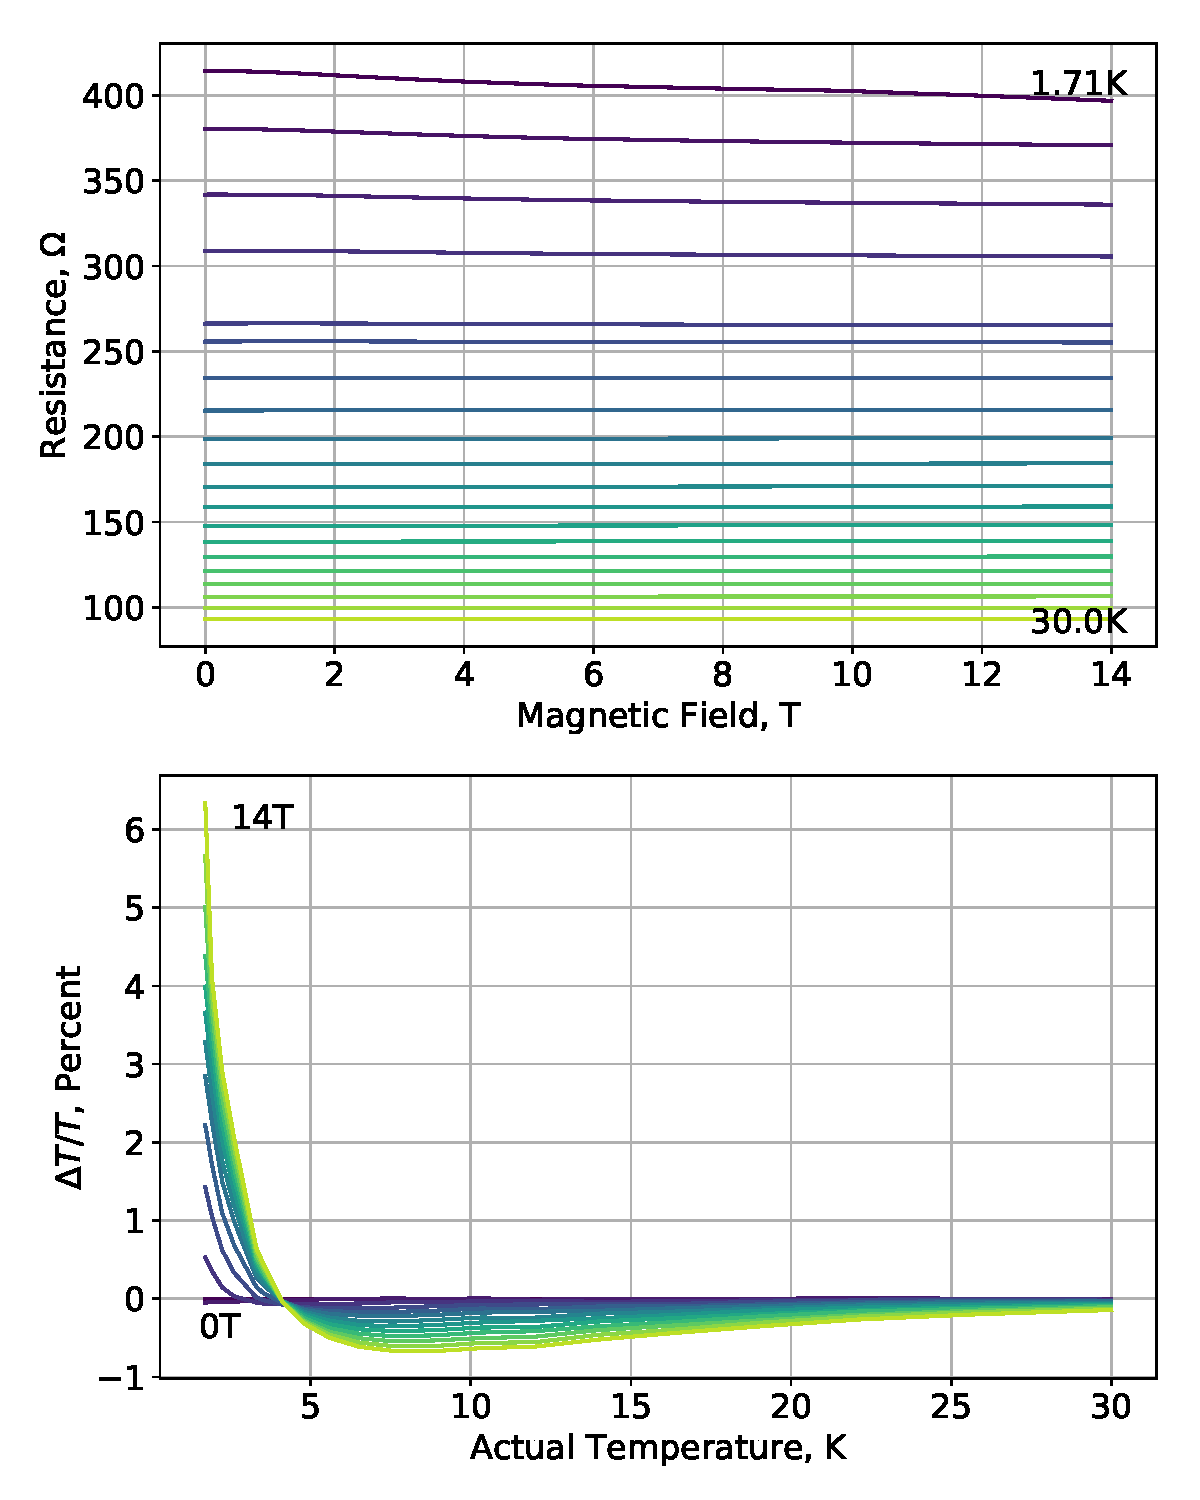
\includegraphics[width=\textwidth]{figures/cal_cernox_1.pdf}
\caption[Example Cernox Field Calibration]{Example Cernox Field Calibration. Top: Magnetoresistance of a
Cernox thermometer. Bottom: Field calibration curves for the same
thermometer.
\((T_{\mathrm{apparent}} - T_{\mathrm{actual}})/T_{\mathrm{actual}}\) is
plotted versus the actual temperature. \label{cernox_fieldcal}}
\end{figure}

Regardless, there is a great deal of scientific value in thermal
measurments performed in strong magnetic fields. Heat capacity provides
a generic method for identifying phase transitions, and thermal
transport is sensitive to excitations in a solid which do not carry
charge and thus can't be studied with electrical transport methods.
Thus, it is our goal to develop new methods for accurately and precisely
measuring temperature in the presence of intense magnetic fields. The
scientific potential of these methods and the experimental techniques
they make possible will be underscored in the next section. For more
information about thermometry and its application in experimental
condensed matter physics, chapter 5 of \cite{Ekin2006} is an invaluable
reference.

\section{Quantum Criticality in Strontium Titanate}

With the goal of identifying a system with some observable quantity which is sensitive to temperature but not magnetic field in mind, we turn to the theory of quantum critical ferroelectricity in strontium titanate (SrTiO$_3$). Strontium titanate is well known as a paraelectric, a material where an applied electric field $\mathbf{E}$ gernates a polarization density, or electric dipole moment per unit volume $\mathbf{P}$:
\[ \mathbf{P} = \epsilon_0 \chi_e \mathbf{E} \]
where $\epsilon_0$ is the permittivity of free space and $\chi_e$ is the electric susceptiblity. Note that the electric susceptibility is a unitless quantity, the fundimental constant $\epsilon_0$ converts the units between $\mathbf{E}$ and $\mathbf{P}$. Strontium titanate (abrieviated STO) has been known to have a large electric susceptibility of 330 at room temperature that rapidly increases as the temperature is lowered~\cite{Neville1972}. This indicates that it might be useful for making a capactive thermometer, as for a parallel plate capacitor, the capactitance is given by
\[ C = \frac{\epsilon A}{d} = \frac{\epsilon_0(1+\chi_e)A}{d}\]
where $A$ is the area of the plates, $d$ is the distance between them, and $\epsilon = \epsilon_0 (1 + \chi_e)$ is the permittivity of the medium between the plates. However, it is worth discussing what the origin of this large electric susceptiblity in STO. The electric susceptibility is intimately connected with the optical phonons of a crystal, since it is these phonons which decribe displacements of the ions in the unit cell relative to each other and can thus produce a net electric dipole in an ionic crystal~\cite{AshcroftMermin}. It is not immediately obvious why these should depend so strongly on temperature, however.

One significant hint comes from the fact that some crystals with the same perovskite structure as strontium titanate, such as barium titanate and lead titanate, are ferroelectrics, i. e. materials which maintain a spontaneous polarization density without the application of an electric field~\cite{Jona1962}. This is analogous to the spontaneous magnetic dipole moment present in ferromagnets such as iron. These materials are so called displacive ferroelectrics, where the net dipole moment is the result of a displacement in the lattice. This corresponds to having an optical phonon with zero frequency. Above the Curie temperature $T_c$, these materials are paraelectrics similar to strontium titanate, with dielectric susceptiblities that are proportional to $(T - T_c)^{-1}$. In qualitative terms, this results from a temperature dependent gap opening up in the optical phonon spectrum, from an optical phonon with zero frequency below $T_c$ to a ``soft'' optical phonon above $T_c$~\cite{RowleyThesis}. This would result in a material which has a strongly varying dielectric susceptibitily with temperature, but in any event strontium titanate does not have a spontaneous electric dipole moment. Additionally, as will be seen in measurements described below, the temperature dependence of strontium titanate does not go as $\chi_e \sim 1/T$, but $\chi_e \sim 1/T^2$!  
\begin{figure}
	\centering
	\caption[Quantum Critical Ferroelectric Phase Diagram]{Phase diagram of quantum critical ferroelectricity, reproduced from~\cite{Rowley2014}. On the x axis, the tuning parameter is derived from the Debye wavevector $\Lambda$ and parameters from the electric polarization equation of state $a$ and $c$. Note the position of Strontium Titanate outside the ferroelectric regime.}
	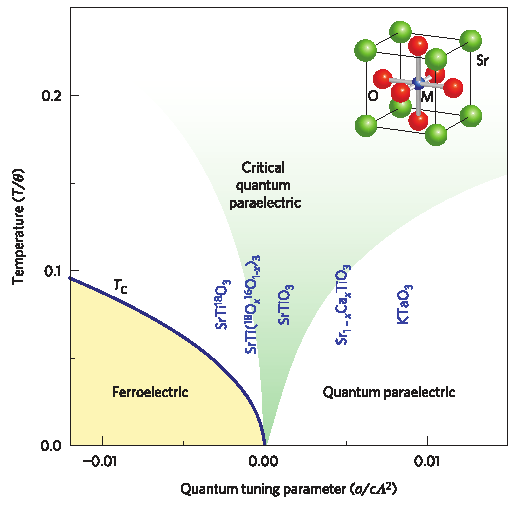
\includegraphics[width=0.6\columnwidth]{figures/sto_phasedia_rowley.pdf}
\end{figure}

\begin{figure}
	\caption[Dielectric constant of Strontium Titanate]{Top: Dielectric constant of Strontium Titanate as a function
		of temperature, plotted as 1/$\epsilon$ vs $T^2$ to show the
		linear trend. Bottom: Low temperature plot of $1/\epsilon$,
		showing that $\epsilon$ reaches a maximum at $T = 3.29$K. This
		data was taken using the VTI probe in our Janis cryostat, but
		reproduces the results of ~\cite{Rowley2014}.}
		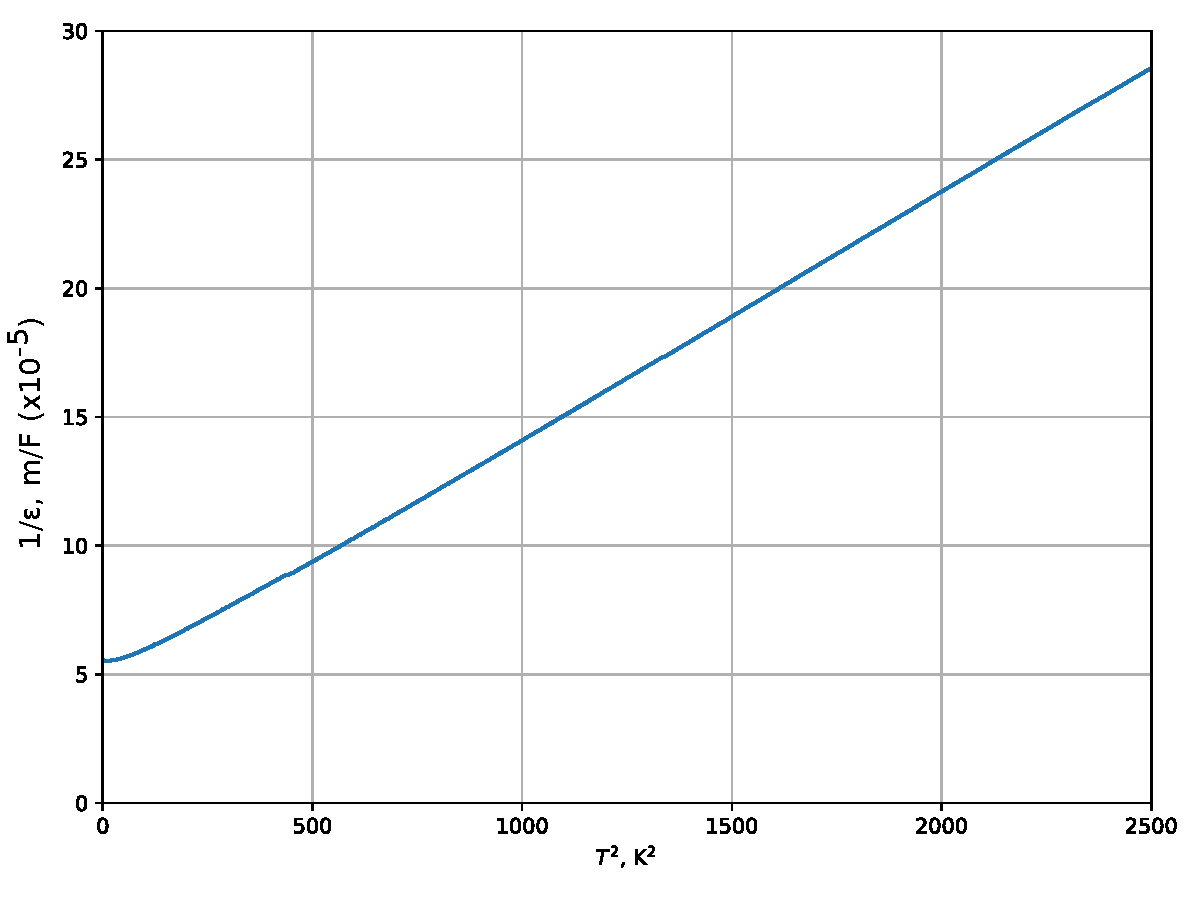
\includegraphics[width=0.9\columnwidth]{figures/STO_eps_vs_T.pdf}
		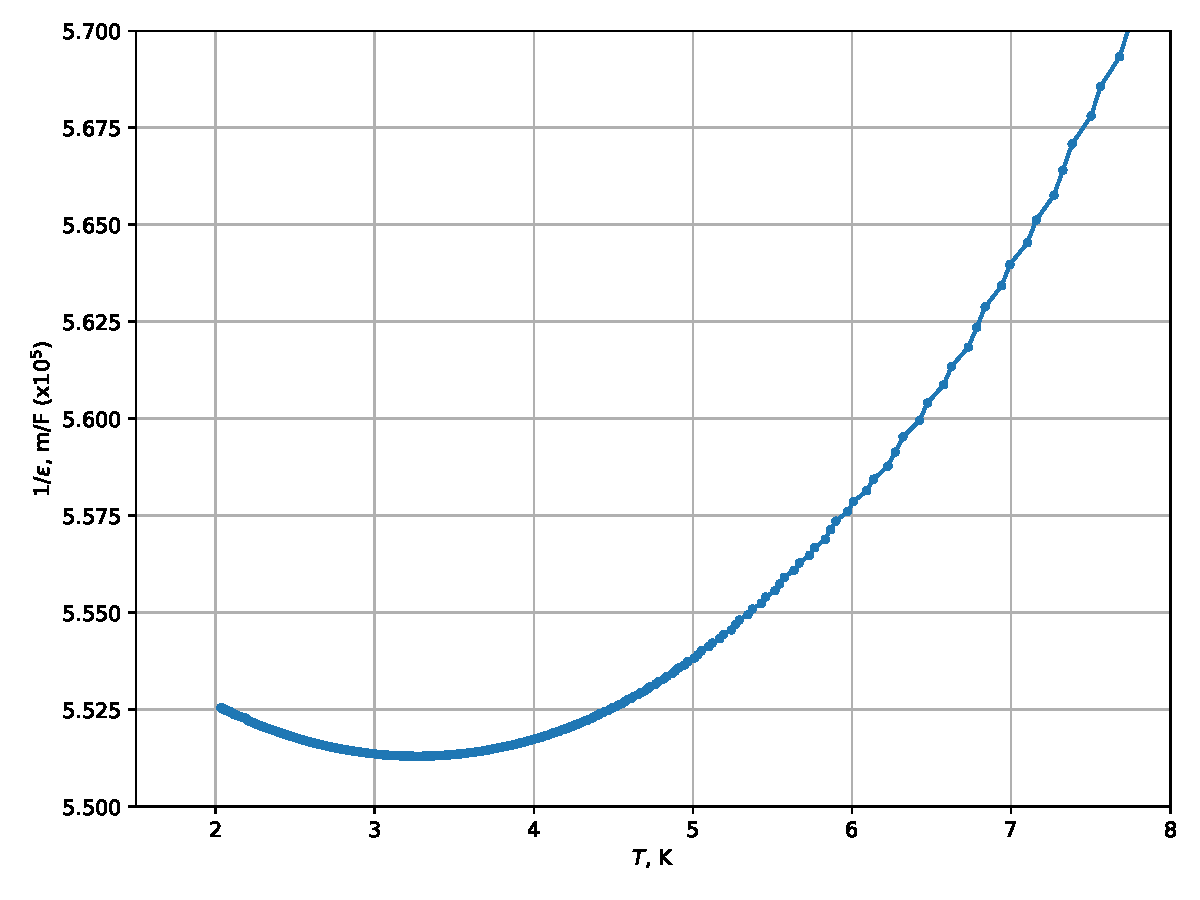
\includegraphics[width=0.9\columnwidth]{figures/STO_eps_vs_T_low.pdf}
		\label{sto_eps_vs_T} \end{figure}

\begin{figure}
\caption[Sensitivity of STO test device]{Sensitivity of the Strontium Titanate device under test, plotted as the ``dimensionless'' quantity \(\frac{1}{C} \frac{dC}{dT}\).}
	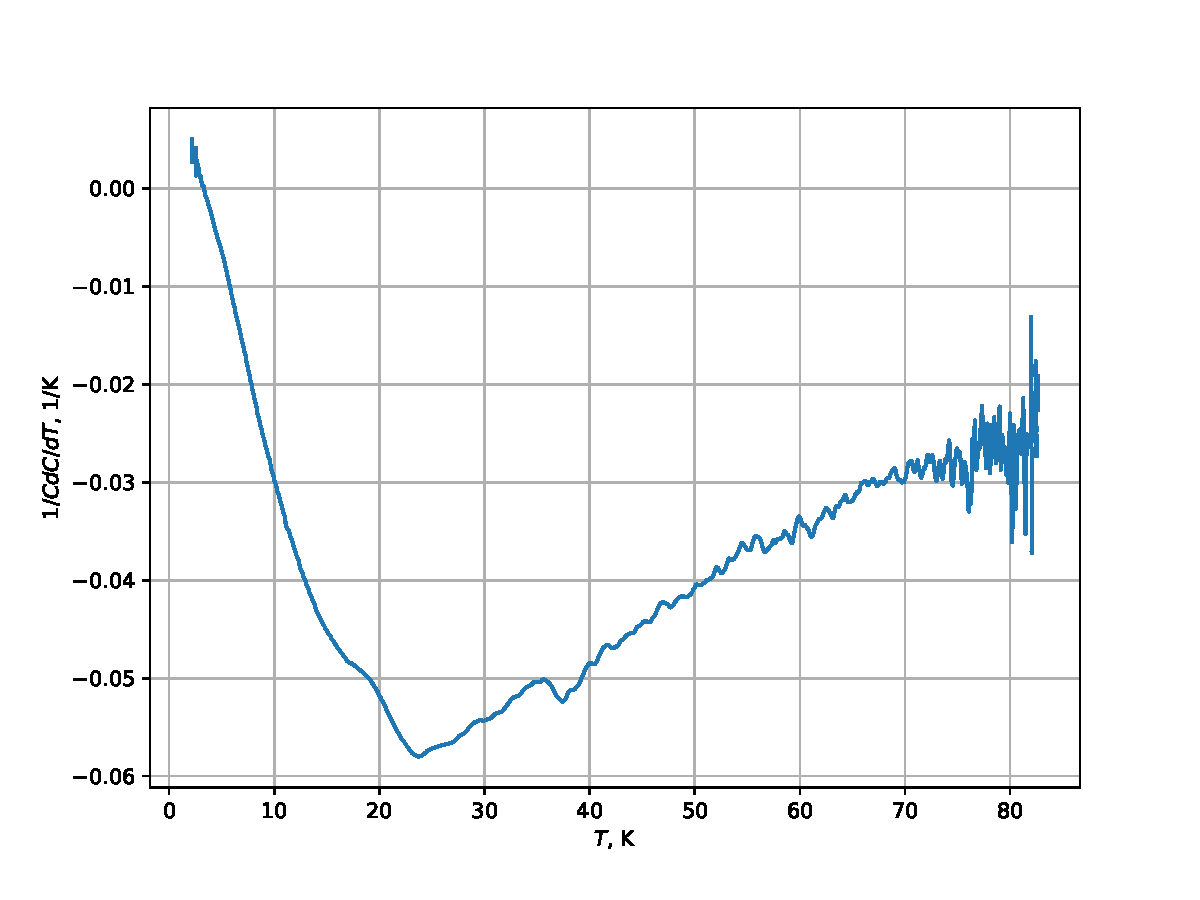
\includegraphics[width=\columnwidth]{figures/STO_dCdT_vs_T.pdf}
\end{figure}

\begin{figure} \caption[Dielectric constant of Potassium Tantalate]{Top: Dielectric constant of Potassium Tantalate
		(KTaO$_3$), another paraelectric material considered as a
		candidate for making capacitve thermometers. The linear trend
		when plotted as 1/$\epsilon$ vs $T^2$ is not as apparent as for
		SrTiO$_3$, and the overall change is not nearly as large.
		Bottom: Low temperature plot of $1/\epsilon$, as in figure
		\ref{sto_eps_vs_T}. The dielectric susceptiblity reaches a
		maximum at $T = 4.31$K, higher than that in SrTiO$_3$. As
		before, this data was taken using the VTI probe in our Janis
		cryostat, but reproduces the results of ~\cite{Rowley2014}.}
	
	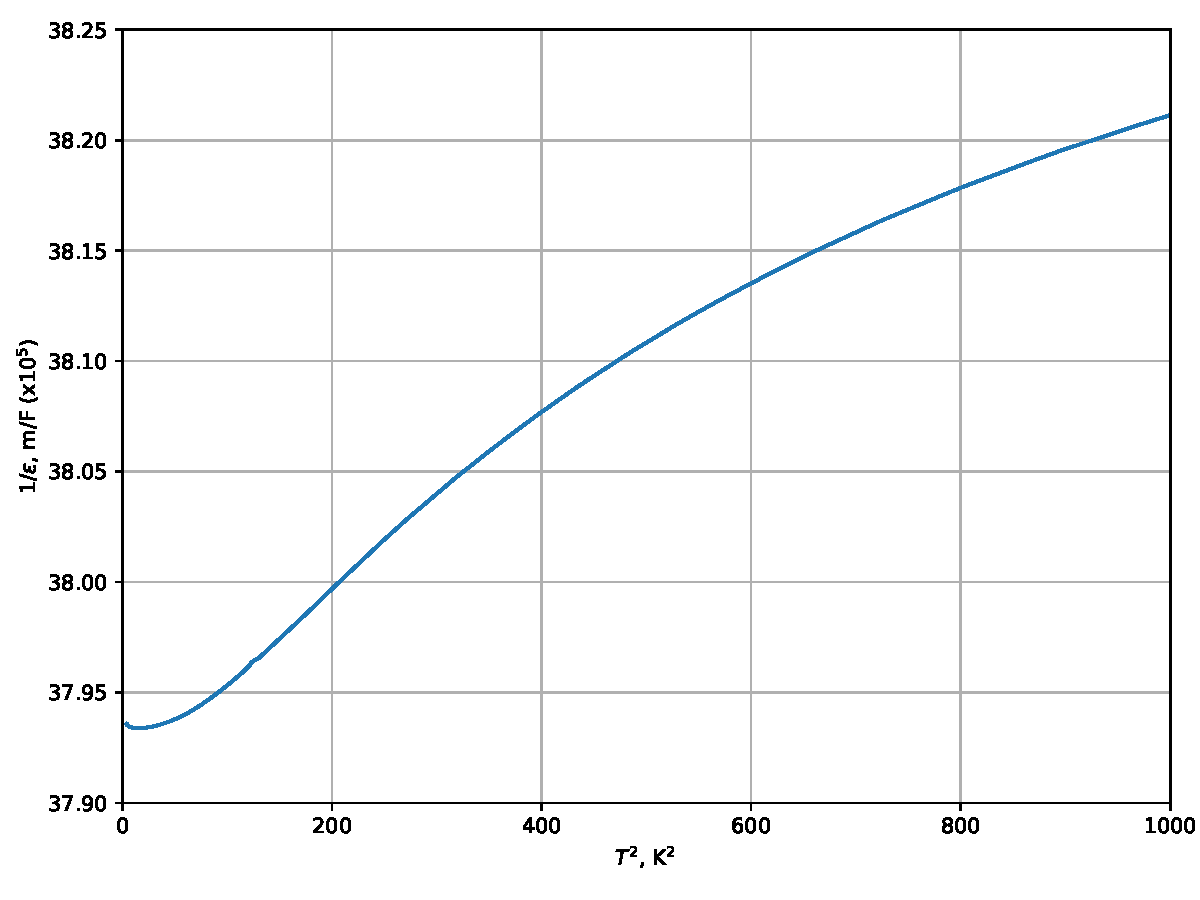
\includegraphics[width=0.85\columnwidth]{figures/KTO_eps_vs_T.pdf}
	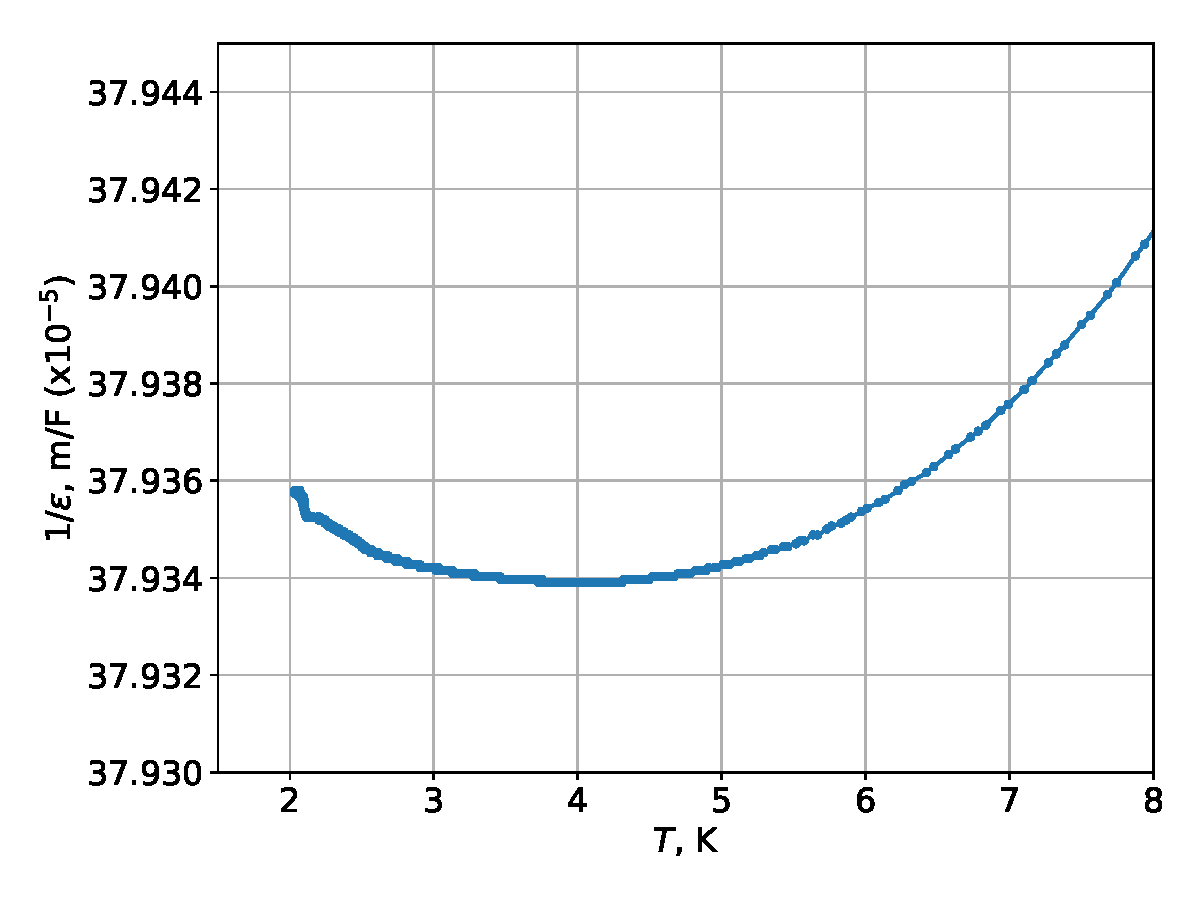
\includegraphics[width=0.85\columnwidth]{figures/KTO_eps_vs_T_low.pdf}
\end{figure}

\section{Electronics For Measuring Capacitance}

\section{Strontium Titanate Thermometers}

Thermal transport measurements provide a versatile set of methods for probing
the physical properties of matter. Among thermal transport properties, the
thermal Hall effect shows promise for probing the ground state of many materials
of physical interest.  The thermal Hall effect, also known as the Righi-Leduc
effect,  is a thermal analogue of the standard Hall effect in which a thermal
gradient is applied across a sample in a magnetic field resulting a secondary
orthogonal thermal gradient. In this sense, a thermal Hall conductivity
$\kappa_{xy}$ is analogous to the Hall conductivity $\sigma_{xy}$.  While
$\sigma_{xy}$ in general contains information about the charged excitations
(electrons or holes) in a material, $\kappa_{xy}$ in principle contains
information about all the low-energy excitations. As a result the thermal Hall
effect has been of great theoretical interest for several years. In particular,
there has been some work that indicates that this technique may prove useful for
the study of strongly-correlated topological insulators (TIs) and
high-temperature superconductors. The thermal Hall effect is proposed to reveal
the experimental signature of different kinds of surface states\cite{Wang2014}:
free fermion TIs with a single Dirac cone, and two types of topological
paramagnet with spin-liquid behavior. Traditional Hall effect measurements can
distinguish some of these phases, but specific classification requires
measurement of the thermal Hall conductivity. Further theoretical studies
suggest that the thermal Hall effect could be used to study the quantum phase
transition from an Ising-like state with bosonic excitations to Majorana
fermions in the topological superconductors with supersymmetry~\cite{Grover2014}.

However, despite the intense theoretical interest in the thermal Hall effect,
the technique remains difficult to implement experimentally. A few interesting
measurements have been made in ferromagnets\cite{Onose2010}, frustrated quantum
magnets\cite{Hirschberger2015}, and cuprate superconductors\cite{Cvetkovic2015}, but
the experimental complications of accurately measuring temperature in an intense
magnetic field has prevented the technique from being applied more generally.
Because of the potential value of this technique for studying strongly
correlated materials and other materials of interest, we have sought to devise a
simple method for making these measurements. In particular, we wish to develop a
method which can be used on a wide variety of materials and throughout a large
temperature range, while being independent of the magnetic field.

In order to accomplish this, we have developed thermometers which measure
temperature by measuring the dielectric constant $\epsilon$ of strontium
titanate (SrTiO$_3$). High quality wafers of SrTiO$_3$ are generally available
for purchase, and the material is durable and relatively easy to work with. Its
value as a thermometer comes from the fact that its dielectric constant
increases by up to a few orders of magnitude at low temperature. This comes from
the fact that SrTiO$_3$ is very close to a quantum critical
point\cite{Rowley2014}. Materials similar to SrTiO$_3$, such as Barium Titanate
(BaTiO$_3$), undergo a ferroelectric transition at sufficiently low temperature.
On the other hand, SrTiO$_3$ is classical paraelectric at room temperature, but
is prevented from undergoing a ferroelectric transition due to long-range
interactions suppressing the ferroelectric state, causing it to remain a
(quantum) paraelectric instead. As a result, the dielectric constant does not
diverge a finite temperature, but instead saturates at about 4 K, depending on
the particular sample.

\begin{figure} \caption[A pair of STO thermometers]{A pair of STO thermometers, used to make thermal
  measurements. The background is a piece of graph paper with 1mm divisions, the
thermometers themselves are approximately 0.5 mm long, 0.5 mm wide, and 0.3 mm
thick.} \centering
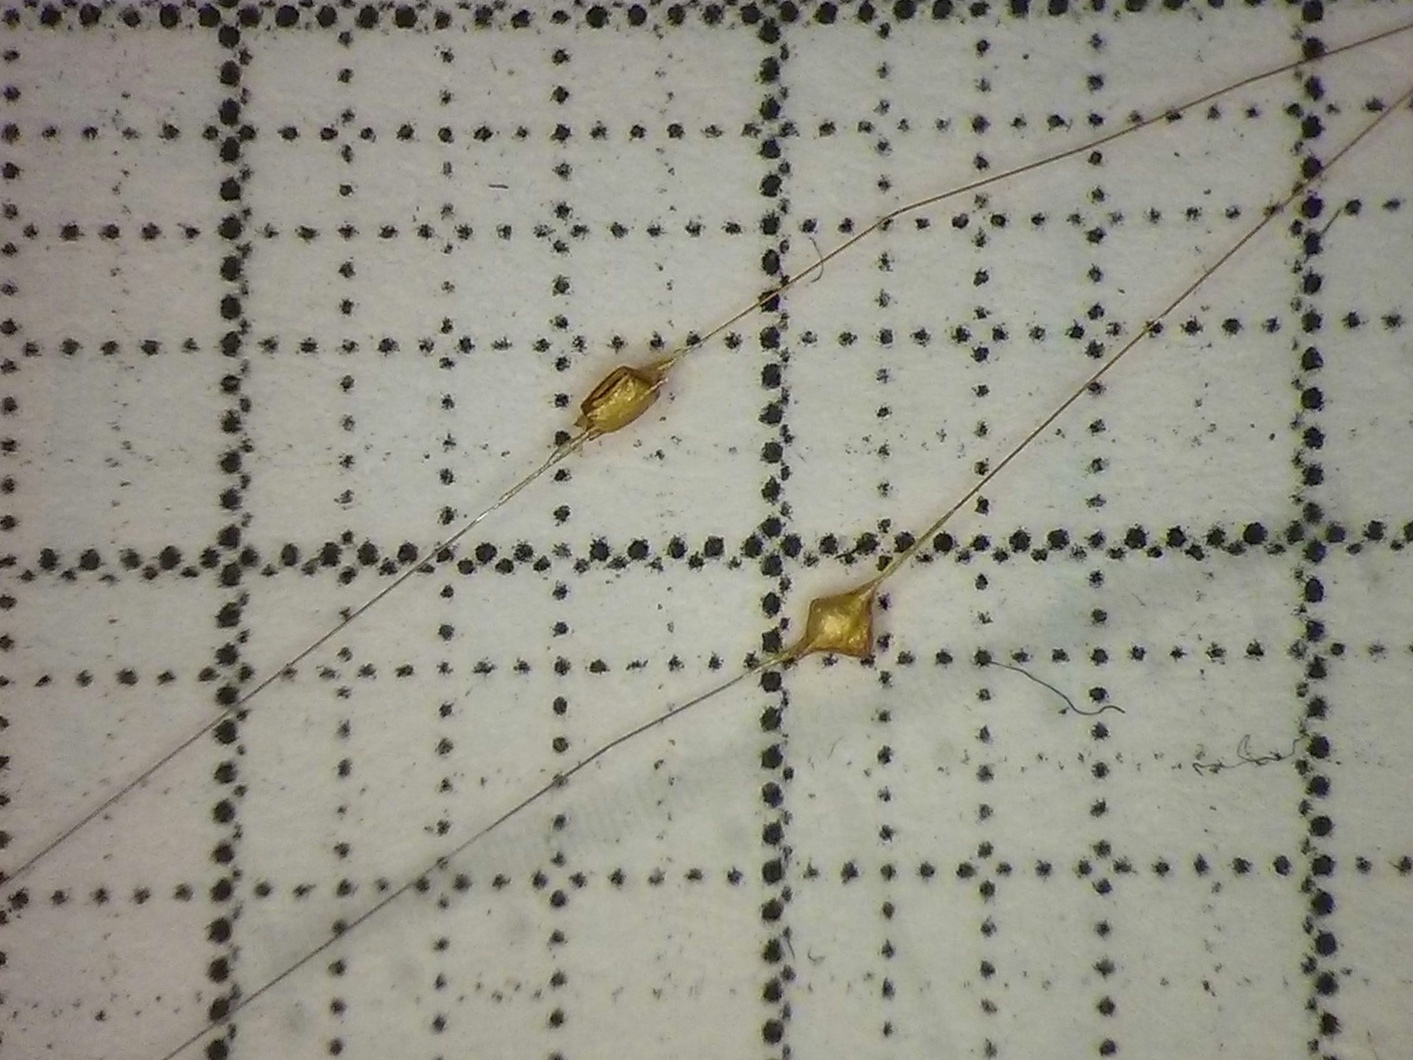
\includegraphics[width=\columnwidth]{figures/thermometers_apl.jpg}\label{thermo_pic}
\end{figure}

\begin{figure} \caption[Example STO thermometer calibration]{An example calibration curve for an STO thermometer,
  showing both the capacitance (solid) and sensitivity (dashed) as a function of
temperature. The capacitance begins to saturate at low temperature, with the
sensitivity peaking around 25K. } \centering
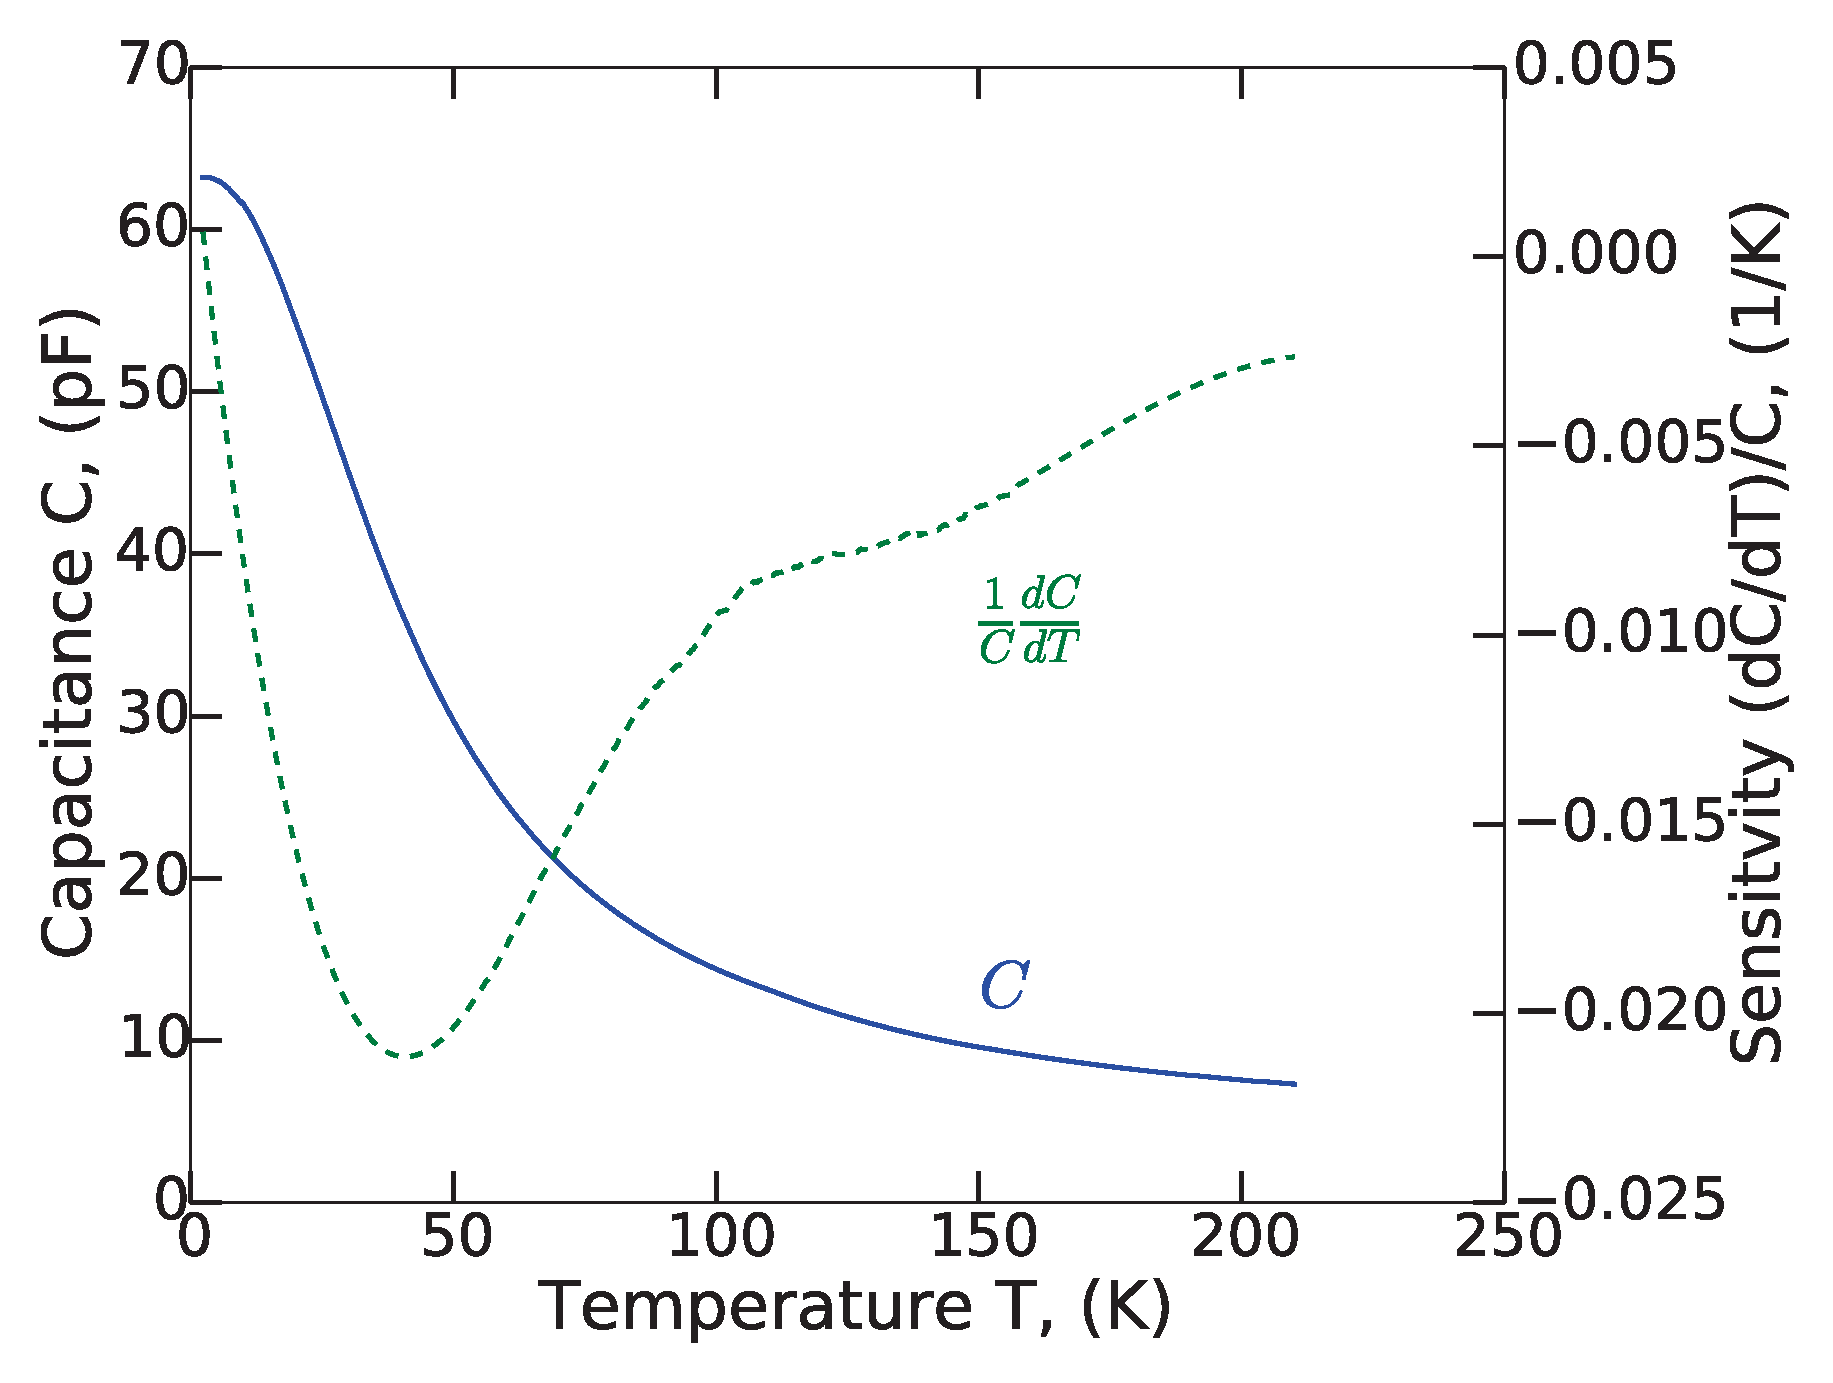
\includegraphics[width=\columnwidth]{figures/cvt_apl.eps}\label{cal_curve}
\end{figure}

In order to make a thermometer out of SrTiO$_3$, we take a small, thin (0.1 mm)
sample of the material (purchased from the MTI corporation)\cite{MTICorp} and
evaporate gold contacts on to either face.  These contacts form a parallel-plate
capacitor, and by measuring the change in the capacitance we measure the
dielectric constant and by proxy the temperature.  Figure~\ref{thermo_pic} shows
a pair of assembled thermometers.  The thermometers are approximately 0.5 mm
long, 0.5 mm wide, and 0.3mm thick, and the electrical leads are a pair of 25
$\mu$m diameter phosphor bronze wires.  Figure~\ref{cal_curve} shows an example
calibration curve for an SrTiO$_3$ thermometer. Both the capacitance and
sensitivity of the thermometer are shown from 4 K up to room temperature. The
magnitude of the sensitivity increases (note the sign, increasing dielectric
constant corresponds to decreasing temperature) up to about 25 K before
decreasing and reaching a maximum value below 4 K. The particulars depend
somewhat on the individual thermometer, notably, some do not reach a maximum
value at all above 1.5 K, the lowest temperature at which we calibrated the
thermometers used in this experiment. We believe this to be due to variance in
our process for making the thermometers, in particular the amount of heat they
are exposed to when the leads are attached and the resin surrounding the wafer
is cured. Because of this, they must be calibrated \textit{in situ} for each
experiment.  However, the general trend is the same, with the sensitivity being
greatest around 20 to 40 K. Using our capacitance bridges (an Andeen-Hagerling
2700A digital bridge and a General Radio 1615-A analog bridge), we can reliably
measure a change in capacitance of about 1$\times$10$^{-5}$ pF. This corresponds
to change in temperature of 0.1 mK. Other measurements~\cite{Hirschberger2015}
using resistive thermometers quote a resolution of 0.2 - 0.4 mK. This is after
extensive field calibration of the thermometers, a time-consuming process which
these thermometers eliminate.

\begin{figure} \caption[Field response of an STO thermometer]{A test of the response of an STO thermometer with a capacitance of 65 pf to an
    applied magnetic field, taken at 4.2K.  The field starts at zero, scans to
    10T (blue), then to -10T (green), and then back to zero (red).  The relative
    change in the capacitance $(C - C_0)/C_0$ remains less than
  3$\times$10$^{-4}$, corresponding to change of about 20 femtofarads. This
change in capacitance is possibly due to the shifting of the leads to the
capacitor plates due to the field, rather than anything intrinsic to STO.}
\centering 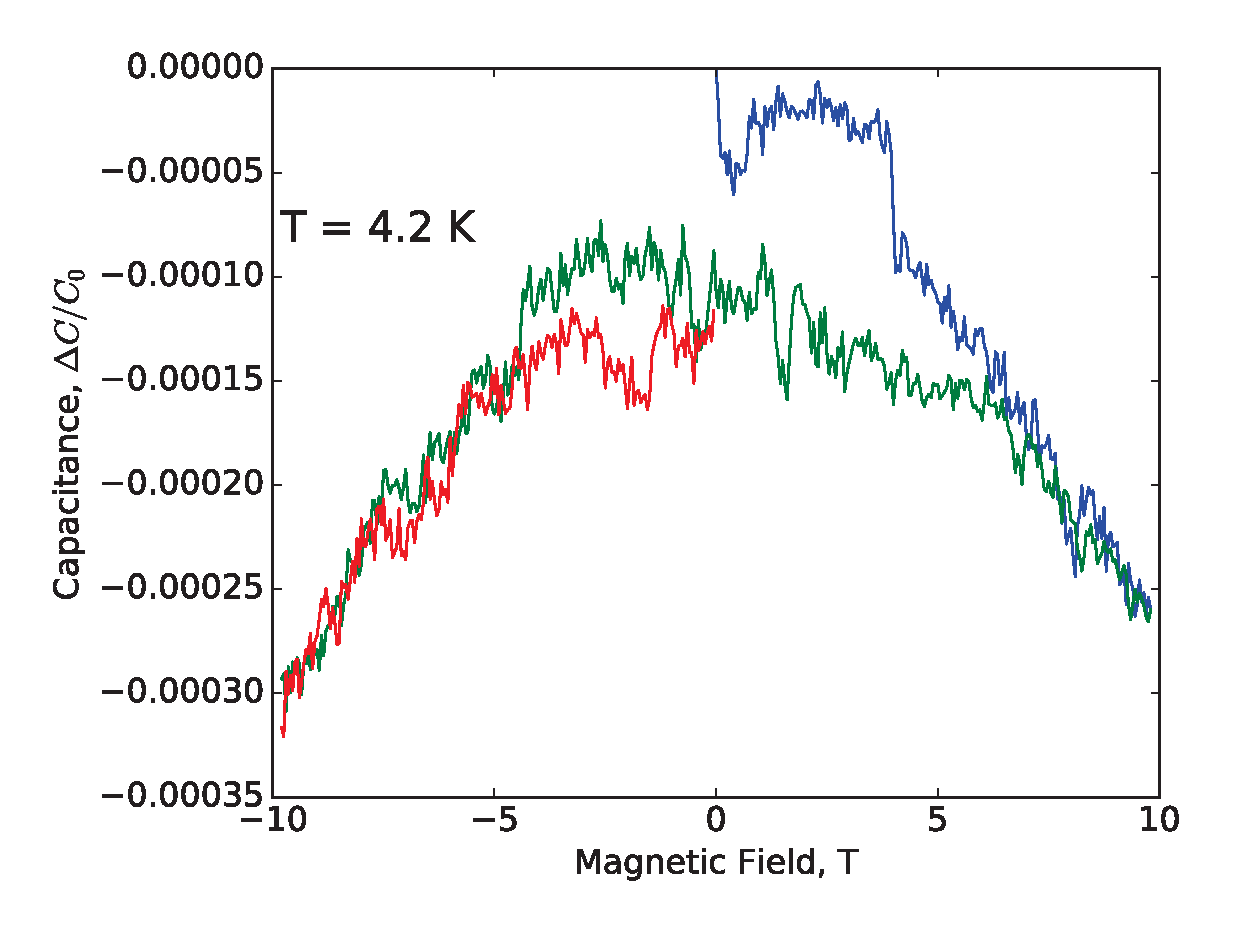
\includegraphics[width=\columnwidth]{figures/cvb_apl.eps}\label{b_test}
\end{figure}

Of course, in order to perform well for making thermal Hall effect measurements,
these thermometers must not be sensitive to an applied magnetic field.
Figure~\ref{b_test} shows the relative change in capacitance $(C-C_0)/C_0$ of a
sample thermometer measured under a magnetic field from -10 T to 10 T.  The
magnitude of the change in capacitance remains less than 3$\times$10$^{-4}$, a
few parts in ten thousand, below 10 T at 2 K. Compare this to resistive
thermometers, which may have magnetoresistance of a few percent or greater in
this temperature range\cite{Heine1998,Goodrich1998}. We are not sure what the nature
of this small field dependence is, as the dielectric constant should be
independent of applied magnetic field. However, at least some of the change may
be related to the slight shifting of the thermometer leads as the field is
swept.

Another issue concerning the suitability of these thermometers for measuring the
thermal Hall effect, particularly relevant at low temperature, is the heating
caused by the thermometers themselves. As the temperature decreases and the
dielectric constant increases, the dissipative losses from the capacitor
increase as well. These increase to about 60 nW at low temperature. For our
current experiment, which applies 1 mW of power across the sample, this is not a
concern. In general, however, this is not insignificant. 60 nW corresponds to an
excitation of 1 V. Decreasing the excitation will quadratically decrease the
heating power, however this comes at the cost of the sensitivity of the device.
This at least gives us some room to adjust the parameters to fit the particular
experiment. As our process for assembling the thermometers improves, we should
be able to mitigate this source of heat by reducing resistive loss across the
capacitor.  Despite the difficulty with the thermometer heating, the fact that
the thermometers are insensitive to magnetic field at low temperature makes them
good candidates for making a variety of thermal measurements.

Furthermore, the heat loss through the thermometer leads are negligible compared
with the sample's thermal conductance. Each thermometer has a pair of 25 $\mu$m
diameter phosphor bronze leads, with a thermal conductivity of 69.9 $\mathrm{W/m
  \cdot K}$ at room temperature given by the manufacturer (California Fine Wire
  Co)~\cite{CFW}. On the other hand, bismuth has a thermal conductivity of 7.87
  $\mathrm{W/m\cdot K}$ at room temperature~\cite{Ekin2006}.  Given the dimensions
  of our sample and the fact that there are two thermometers with four leads
  total, this results in a thermal conductance of 1.6 $\mathrm{mW/K}$ through
  the sample compared to 0.027 $\mathrm{mW/K}$ through the leads, almost 60
  times smaller. Since the thermal conductivity of bismuth goes up below room
  temperature~\cite{White1958}, while that of phosphor bronze goes
  down~\cite{Ekin2006}, the quality will only improve at the measurement
  temperatures.

  \begin{figure} \caption[Transverse temperature gradient of a bismuth crystal]{(Panel a): Transverse temperature difference as a
    function of applied magnetic field from -10 T to 10 T, taken at 130 K and
    measured using a pair of STO thermometers. The signal is composed of an
    symmetric part and an antisymmetric part.  (Panel b): Antisymmetric (solid)
  and symmetric (dashed) parts of the transverse temperature difference. The
antisymmetric part is the thermal Hall signal. Notice the difference in scales
for the two curves.} \centering\label{t_grad}
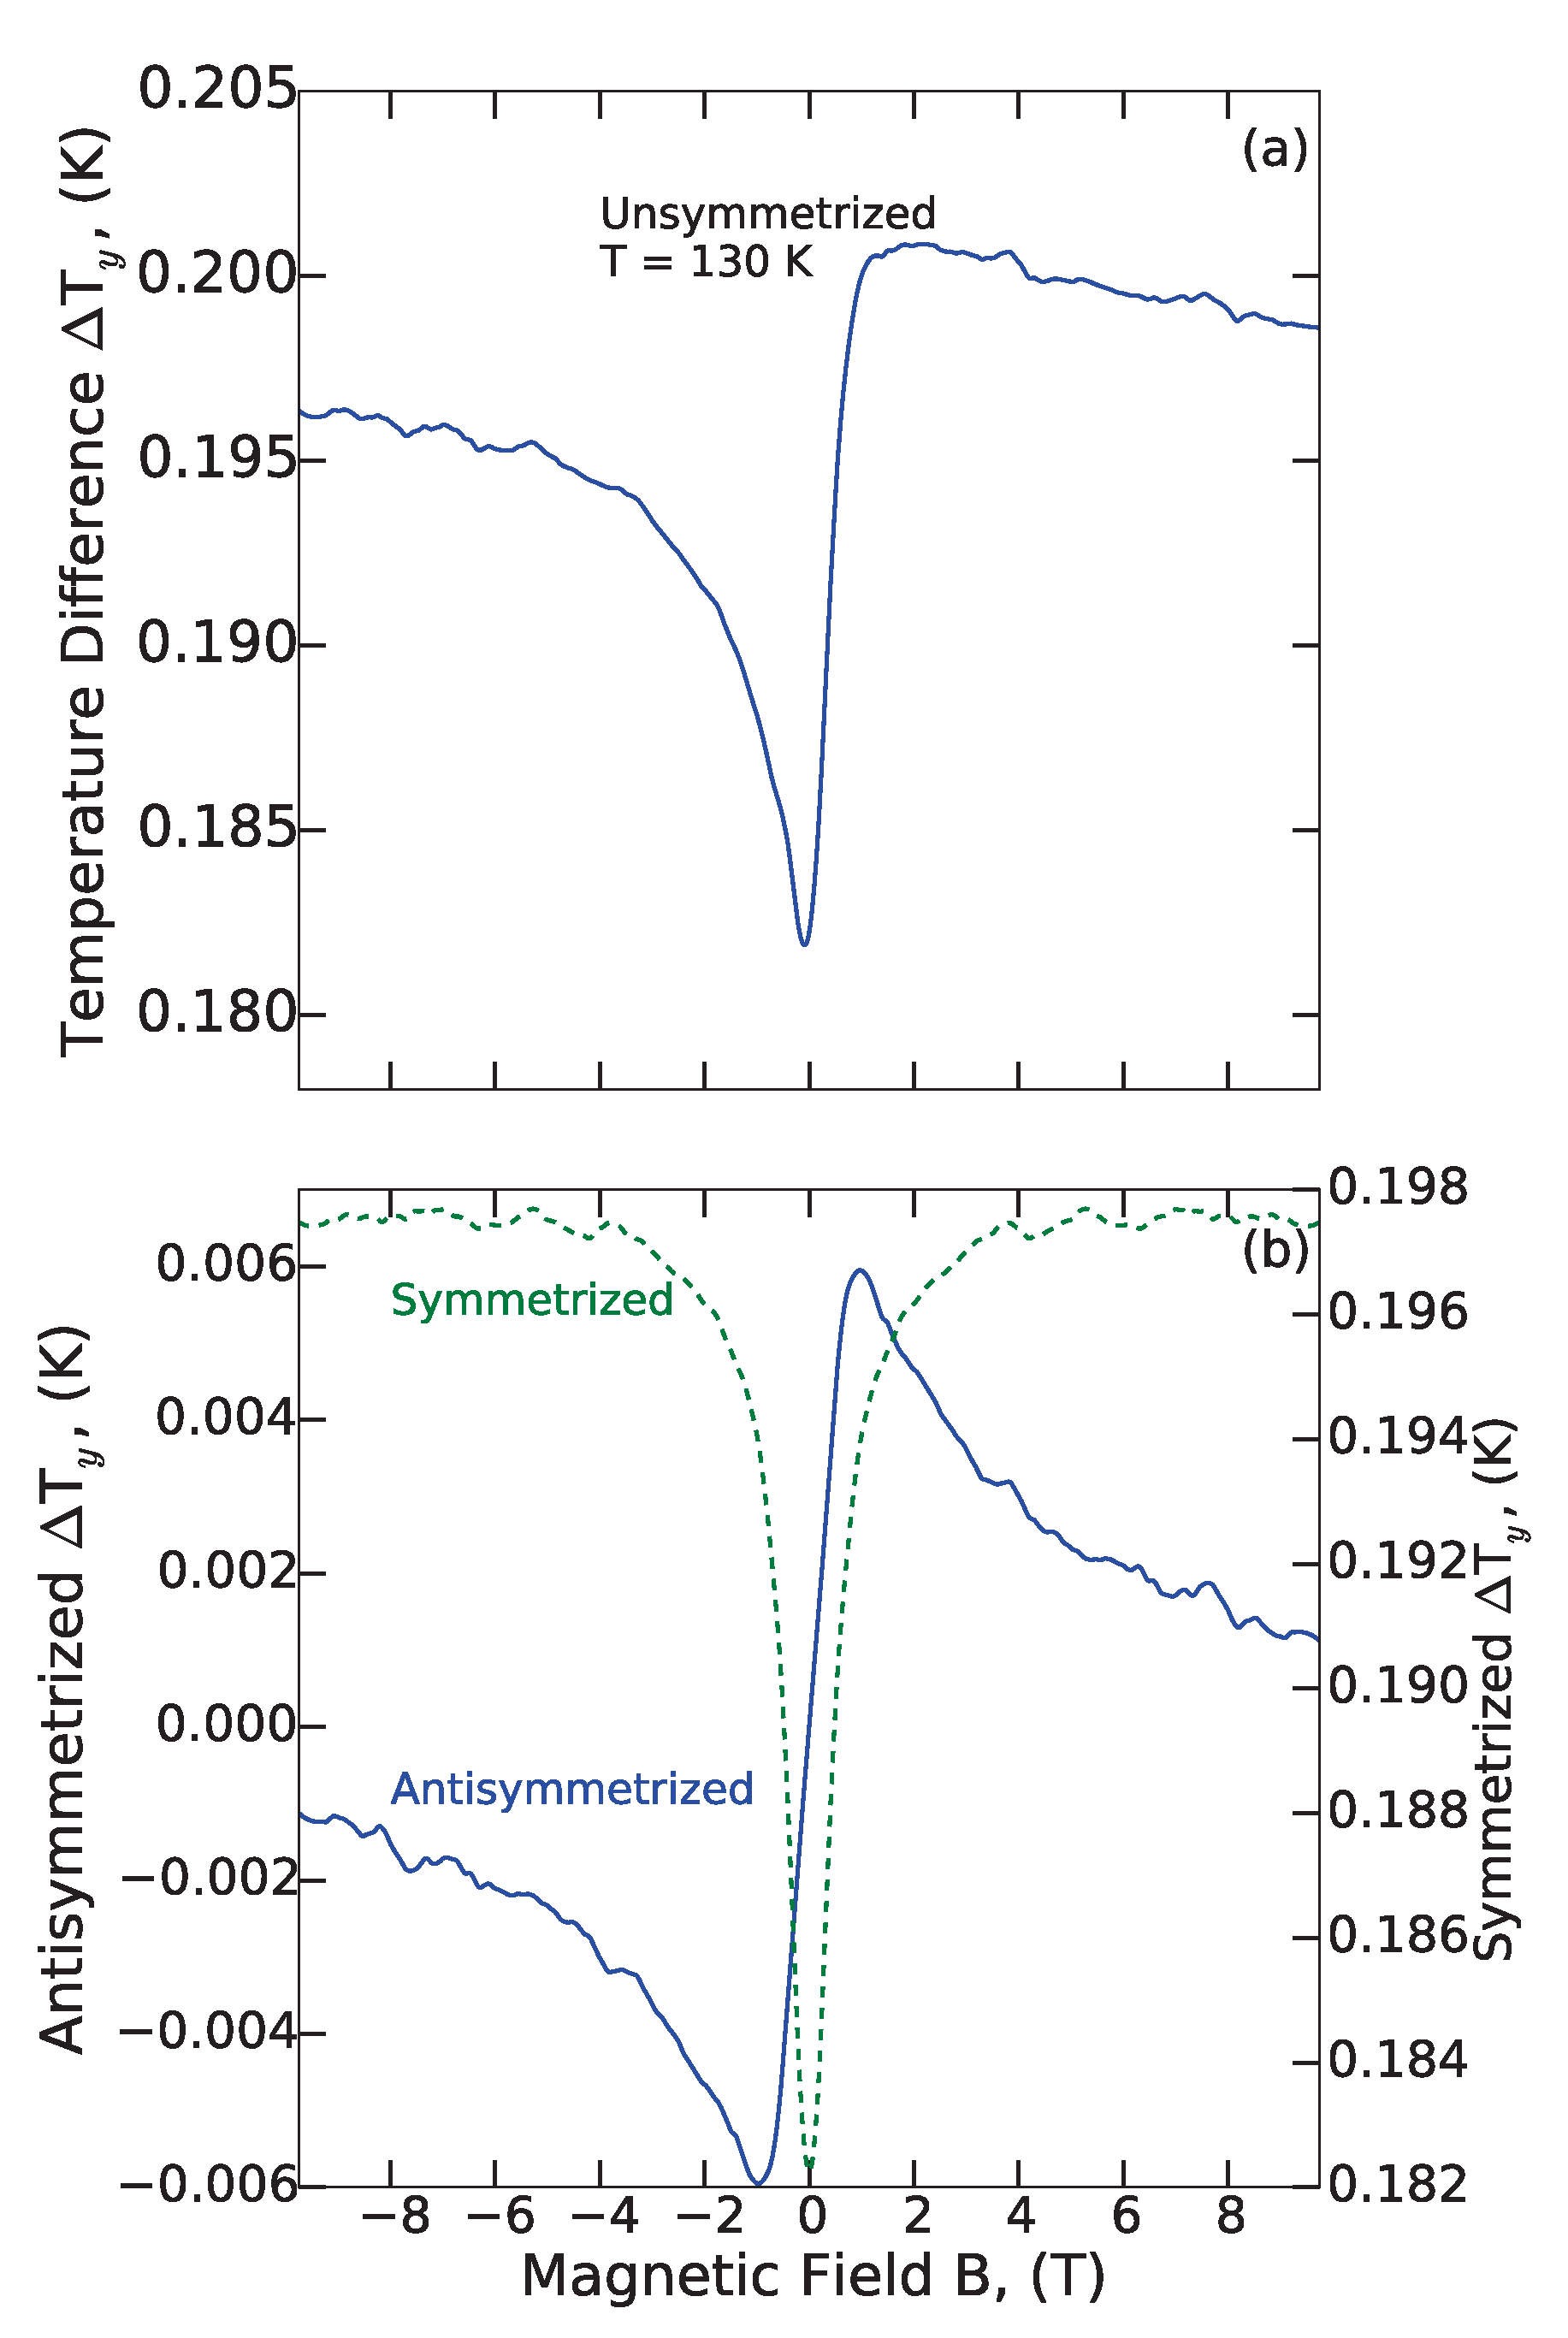
\includegraphics[width=0.9\columnwidth]{figures/rawCurve_apl.eps} \end{figure}

\section{Measuring the Thermal Hall Effect in Bismuth}

As a test of these thermometers' suitability for thermal Hall measurements, we
have measured the thermal Hall coefficient of Bismuth metal. Bismuth is one of
the most studied condensed matter systems, being the material in which a host of
physical phenomena were first discovered. Examples include quantum oscillations
and the de Haas van Alphen effect\cite{deHaas1930}, and perhaps more directly
related to the field of thermal transport measurements, the Seebeck
effect\cite{Seebeck1922}. It has a unique electronic structure, being a semimetal
with Dirac-like dispersion\cite{Lui1995, Li2008}, strong spin-orbit
coupling\cite{Yafet1963}, and pronounced diamagnetism\cite{Shoenberg1936}. More
recently, it has been studied\cite{Emoto2016} for its ability to convert spin
current to charge current along with the ferromagnetic insulator
yttrium-iron-garnet through the inverse spin Hall effect and inverse
Rashba-Edelstein effect. This interplay of electronic, magnetic and thermal
phenomena make bismuth a promising candidate for observing the thermal Hall
effect using our capacitive thermometry technique.

The thermal Hall effect on crystalline bismuth has been carried out by W.
Kobayashi \textit{et al.}\cite{Kobayashi2012} down to 75 K and magnetic fields up
to $\pm$3 T. Using our thermometers, we sought to extend this measurement to
lower temperatures and higher fields. A resistive heater was mounted on a single
crystal of bismuth metal, in order to generate a temperature gradient. A pair of
SrTiO$_3$ thermometers were mounted in order to measure the transverse
temperature gradient. The thermometers were glued to the surface of the sample
and then coated in Type 120 silicone thermal joint compound to ensure good
thermal contact with the sample. An example set of temperature gradient data is
shown in Figure~\ref{t_grad}. Two pairs of thermocouples were mounted as well,
one longitudinal and one transverse, in order to independently measure the
temperature gradients \textit{in situ}. An additional resistive thermometer was
mounted nearby to calibrate the SrTiO$_3$ thermometers in zero field.  The
heater was repeatedly turned on and off, and the gradients in each direction
measured. Simultaneously, the applied magnetic field was swept between -10 T and
10 T. This allowed us to measure the field dependence of the thermal Hall
coefficient.

\begin{figure} \centering \caption[Comparison between thermocouples and STO thermometers]{Transverse temperature differences across a bismuth crystal measured with both STO thermometers (orange) and thermocouples (blue), up to 10T and antisymmetried to isolate the thermal Hall signal. Top: Temperature difference at 110K. At this temperature, the signal is large enough that the thermocouples have no trouble detecting it. The STO thermometers are not so sensitive in this range, and so they have more noise. Bottom: Temperature difference at 30 K. While the thermocouples are not able to detect anything, the STO thermometers are still able to detect a temperature difference of about 0.5 mK.}
	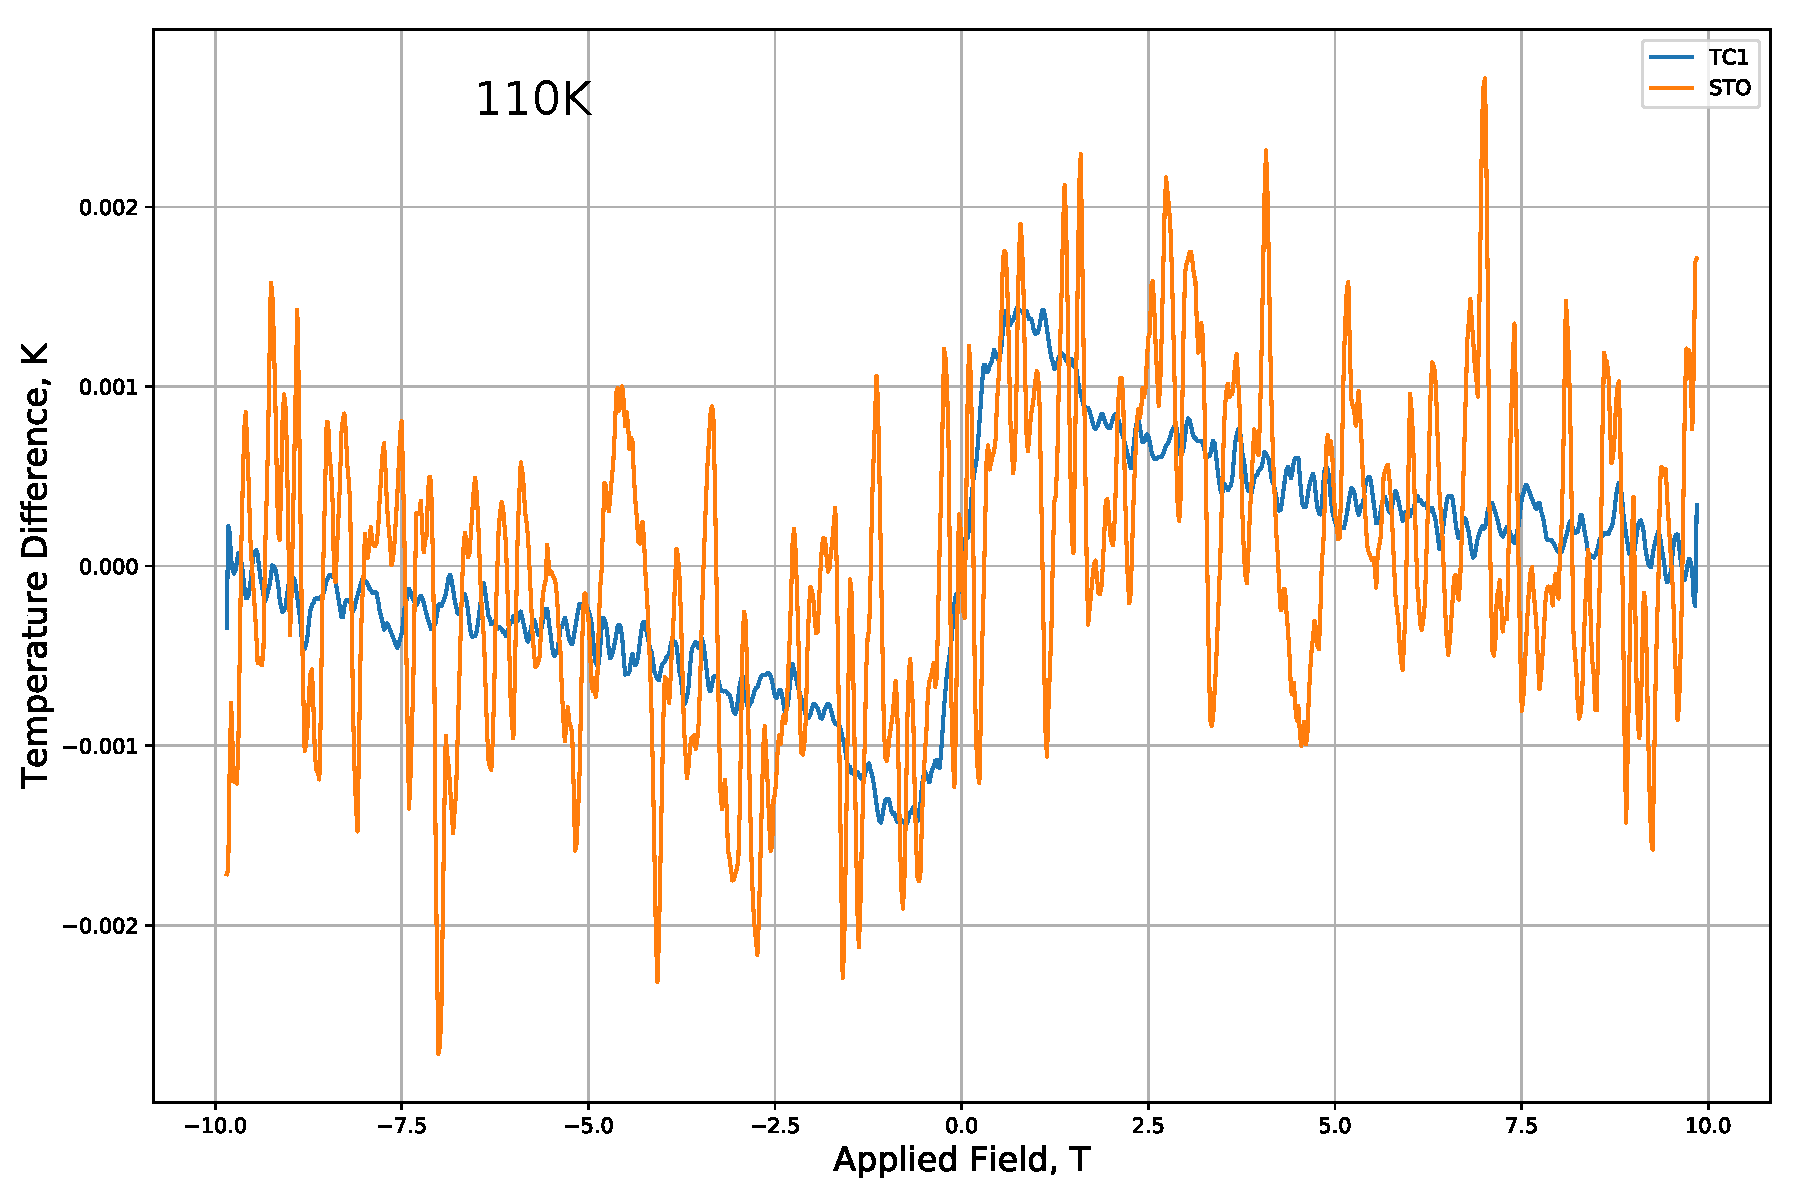
\includegraphics[width=0.9\columnwidth]{figures/110K_HighEx_AntiSym.pdf}
	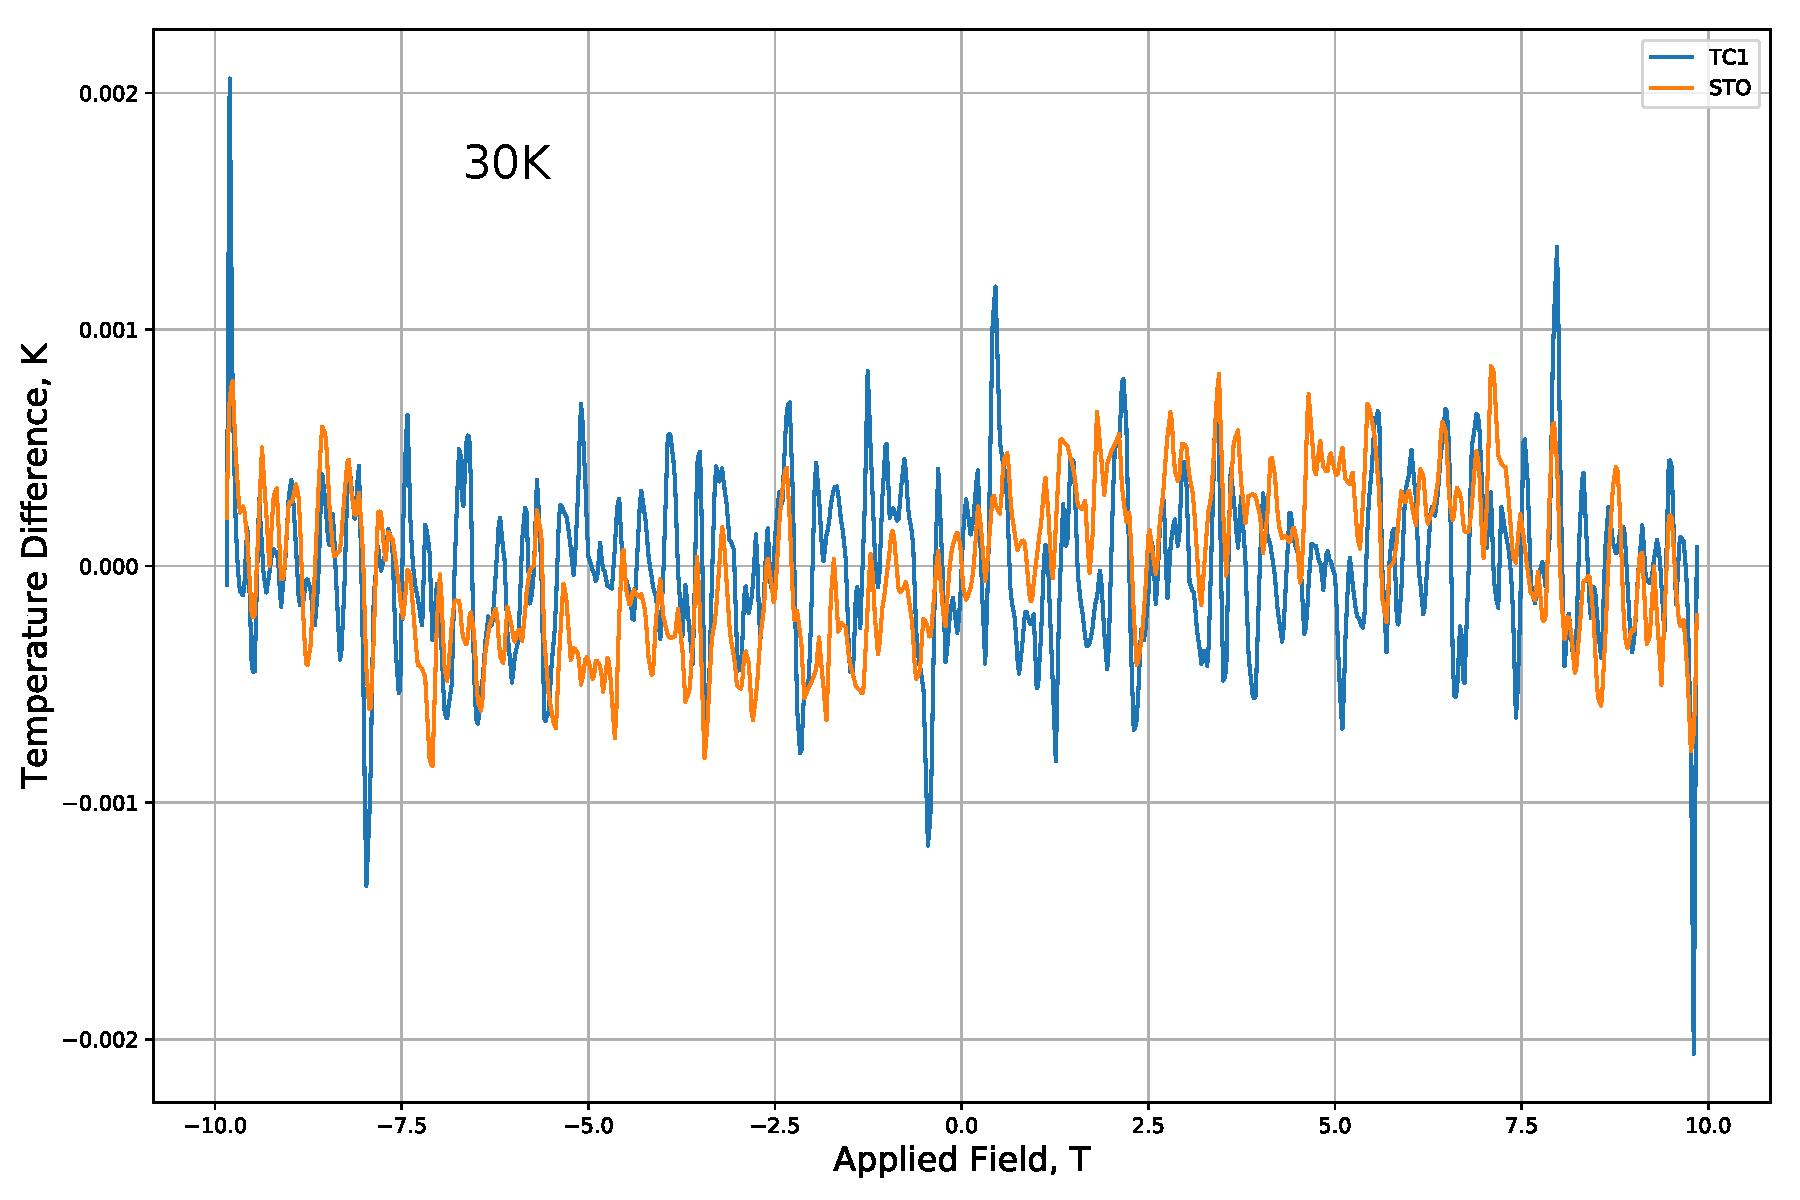
\includegraphics[width=0.9\columnwidth]{figures/30K_HighEx_AntiSym.pdf}
\end{figure}


\begin{figure} \caption[Thermal Hall conductivity of bismuth]{Thermal Hall conductivity, computed from the
    transverse temperature difference measured using the STO thermometers from
    -10 T to 10 T. Curves for a few temperatures between 90K and 175K (Panel a)
    and between 40K and 80K (Panel 6). The signal appears to get smaller at
lower temperature, disappearing at 60K.} \centering\label{kappaxy}
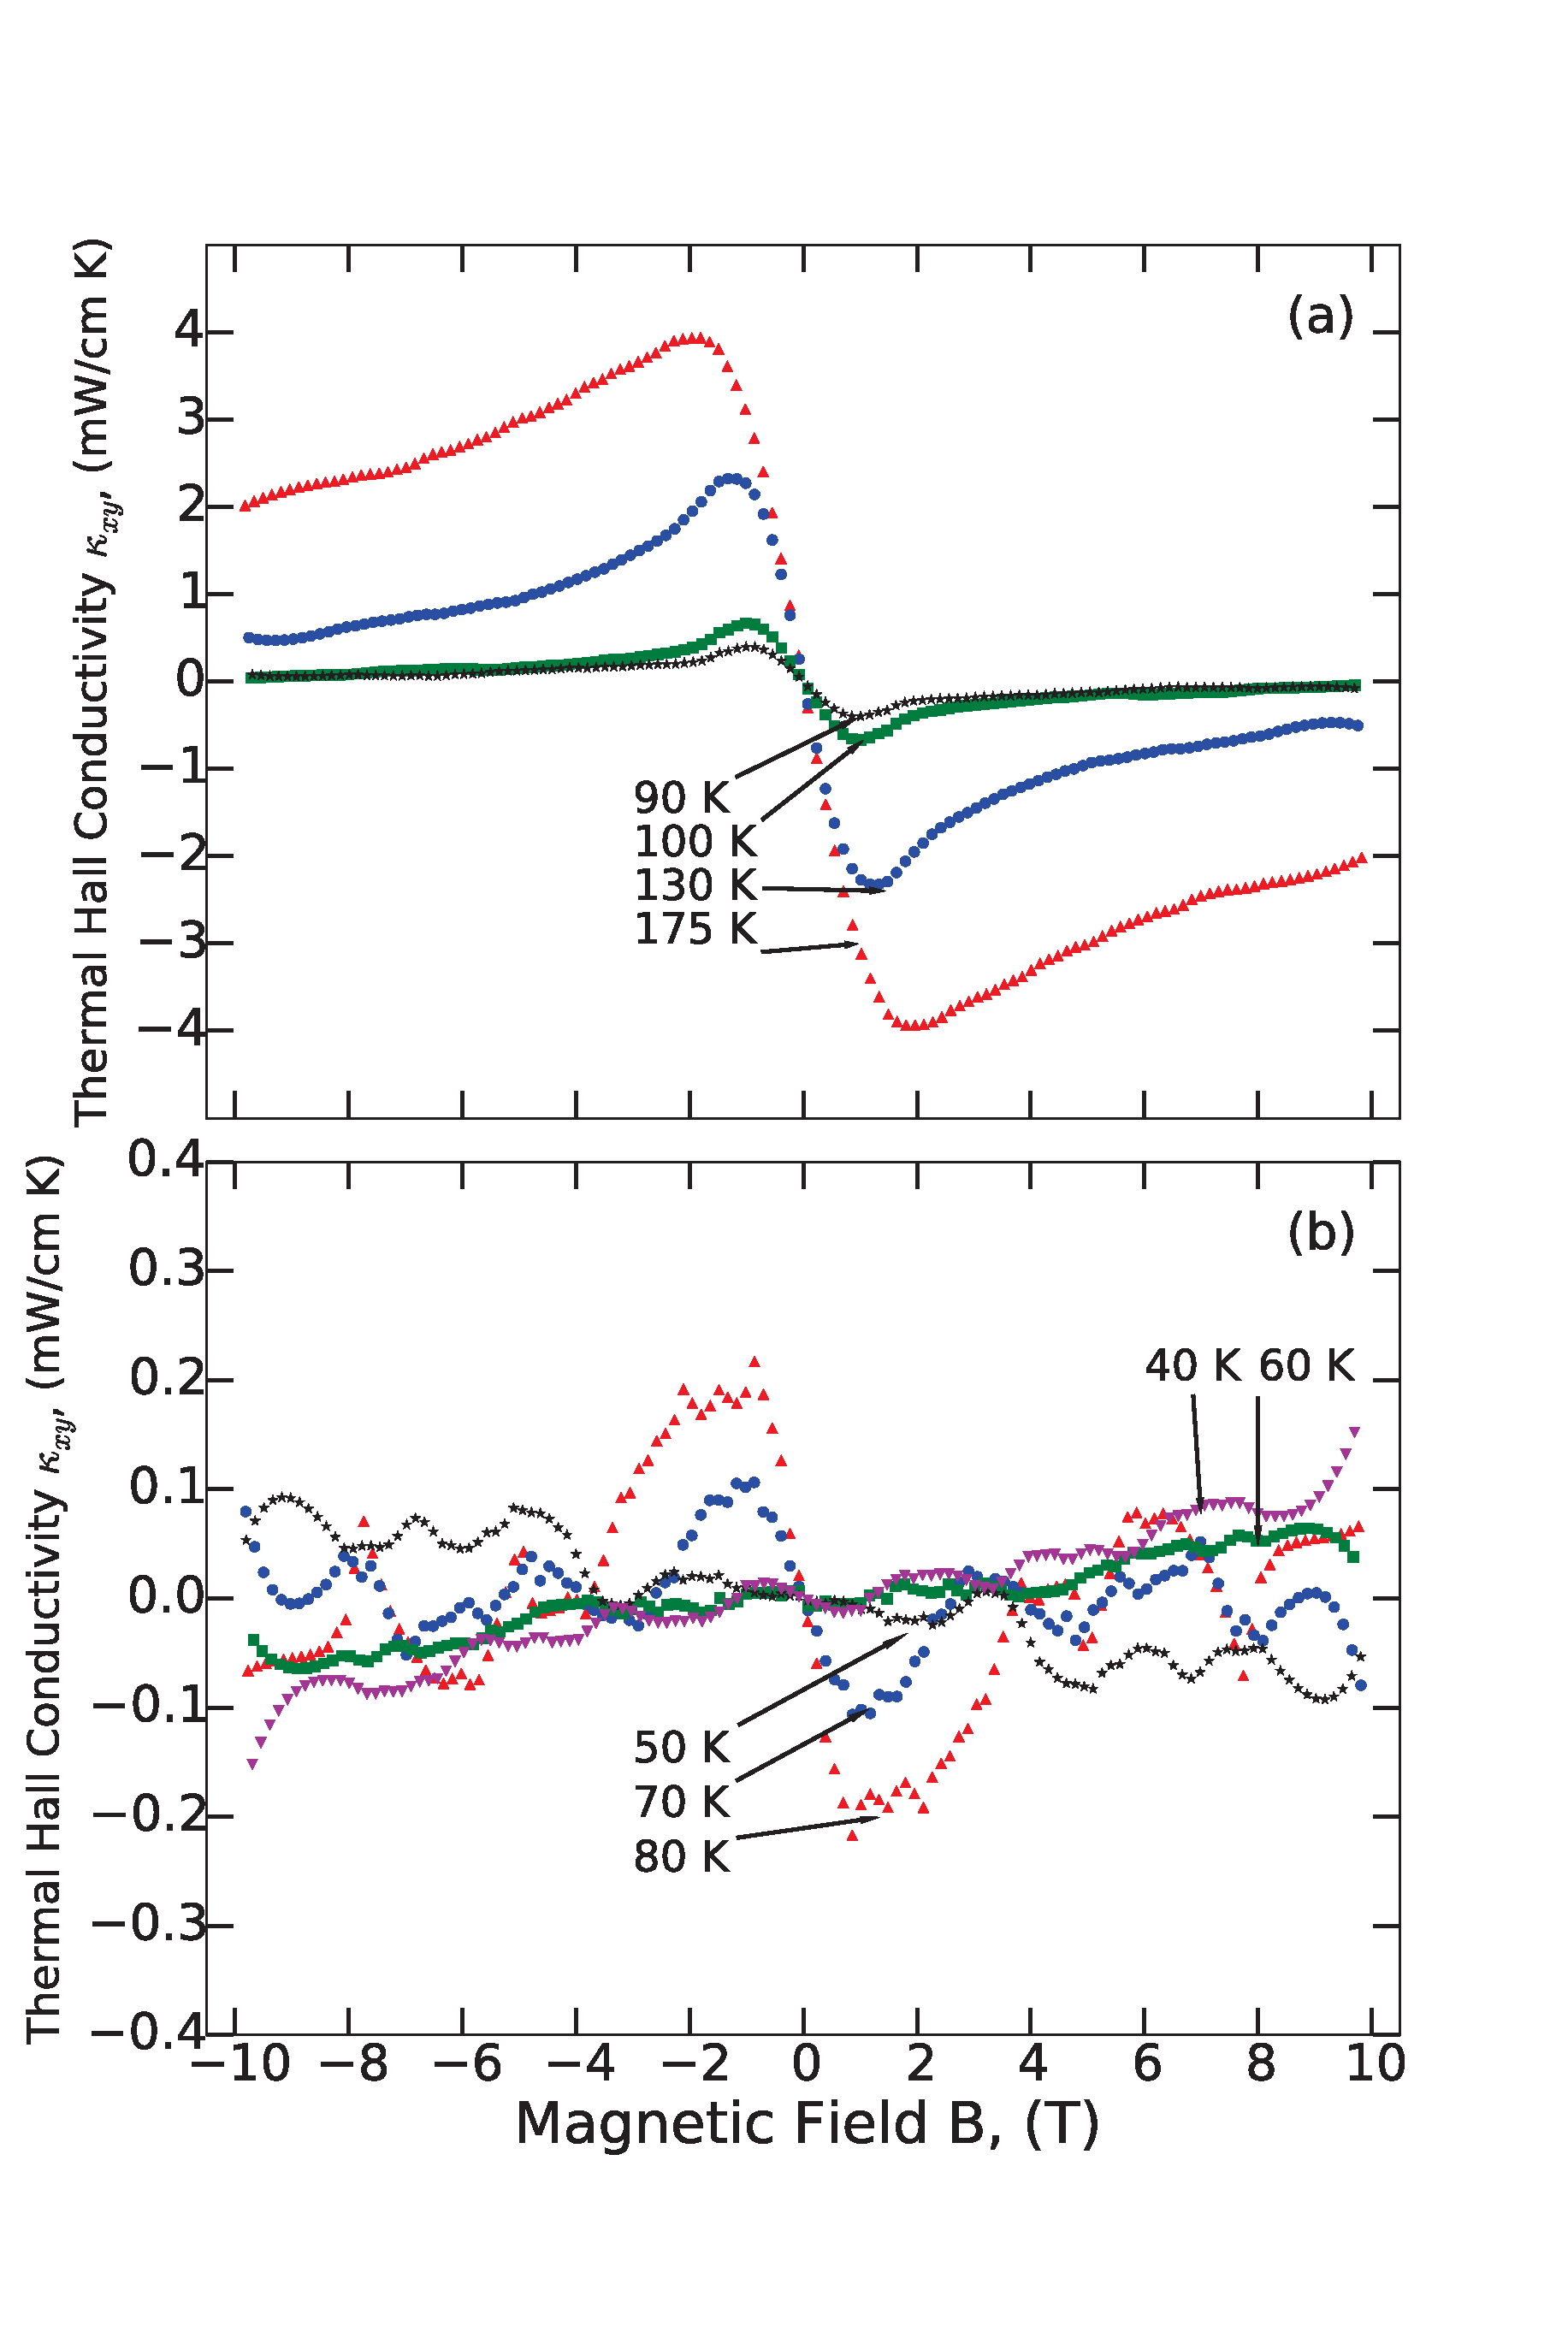
\includegraphics[width=\columnwidth]{figures/kappaxy_apl.eps} \end{figure}

Similar to what was measured before\cite{Kobayashi2012}, the thermal Hall
conductivity is strongly nonlinear, reaching a maximum below 2 Tesla and
decaying down to zero at high field, as shown in Figure~\ref{kappaxy}.  It is
also largest at high temperature, becoming imperceptible below 50 K, where our
thermometers are most sensitive.  As a result, we are confident that this is not
an artifact of the capacitive thermometers. Thus we can see that the STO
thermometers are able to make sensitive measurements, detecting changes in
temperature below 1 mK in magnetic fields up to 10 T. Additionally, the fact
that they are relatively simple to produce makes them applicable to a wide
variety of measurements and samples. One remaining challenge is our ability to
push these measurements to lower temperature, suitable for use at helium-3 or
dilution refrigerator temperatures, where traditional methods of thermometry are
even more fraught\cite{Heine1998, Goodrich1998}. One promising line of study
involved isotopically substituting $^{18}$O into the strontium titanate wafers,
which has been shown\cite{Rowley2014} to drive them closer to the ferroelectric
quantum phase transition and thus continue the divergence of their dielectric
constant to lower and lower temperature. In any event, as this measurement has
shown, this method of thermometry holds great promise for enabling the thermal
properties of materials in intense magnetic fields.

In conclusion, miniature capacitive thermometers based on the paraelectric
material SrTiO$_3$ have been applied to measure the thermal Hall effect in
crystalline bismuth. A strong nonlinear thermal Hall effect is observed in the
intermediate temperature range. The miniature SrTiO$_3$ thermometers show very
little magnetic field dependence -- less than a factor of 3$\times$10$^{-4}$ up
to magnetic field 10 T. They are also quite sensitive, resolving the temperature
difference as little as 0.1 mK.

\section{Annealing Strontium Titanate in Oxygen-18}

\begin{figure} \caption[Strontium Titanate Annealing System]{Schematic of the annealing system used to produce oxygen-18 enriched strontium titanate wafers. The circles labled ``P'' are pressure gauges, and the circles with crosses are valves. Oxygen-18 is supplied from a gas cylinder, and can be stored in the cold trap for reuse.}
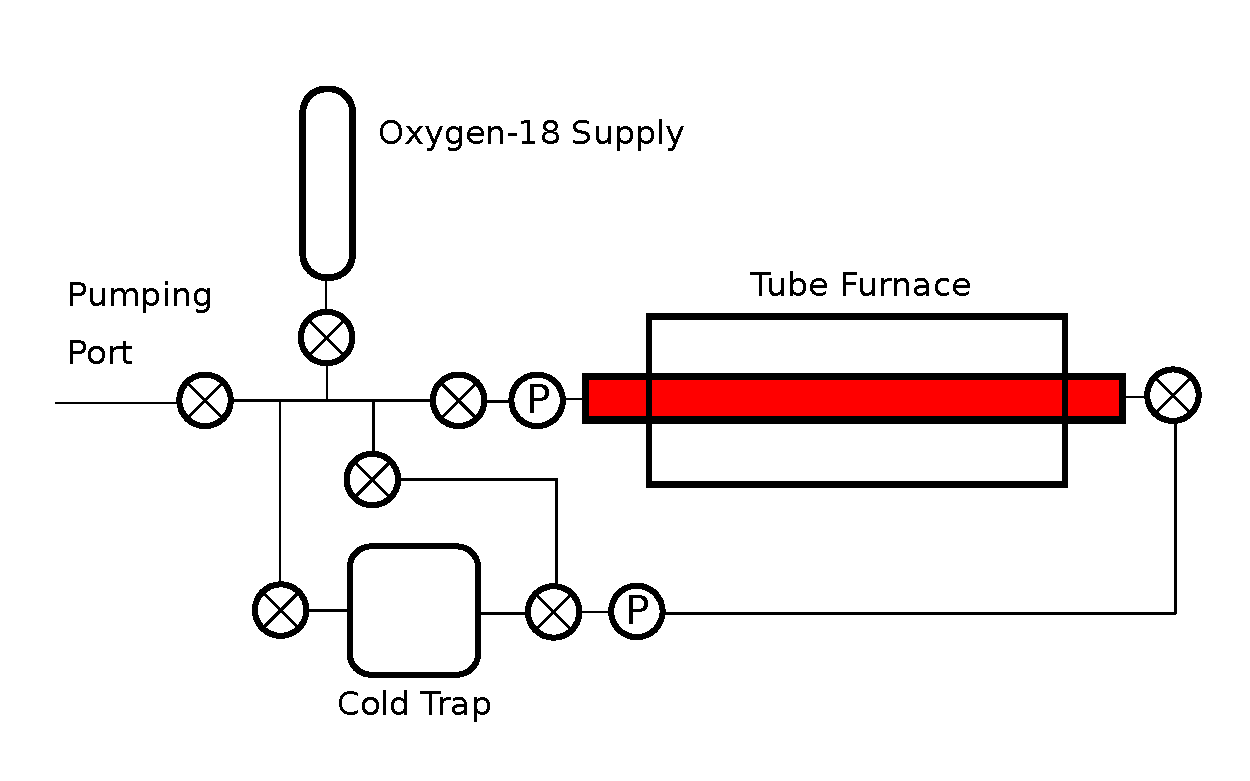
\includegraphics[width=\columnwidth]{figures/annealing_system.pdf}
\end{figure}

\begin{figure} \caption[Annealed STO thermometer reproducability tests]{Top: Reproducability tests for several annealed STO
	capacitor devices, measured in a liquid helium dewar using a dipstick
probe. The Oxygen-18 enrichment percentage is listed in table <TODO>. Note the
offset between the cool down and warm up traces for each device. Bottom:
Sensitivities for the same four devices. Although the capacitance varies
between devices and cool down/warm up, the sensitivity is roughly the same for
each.} 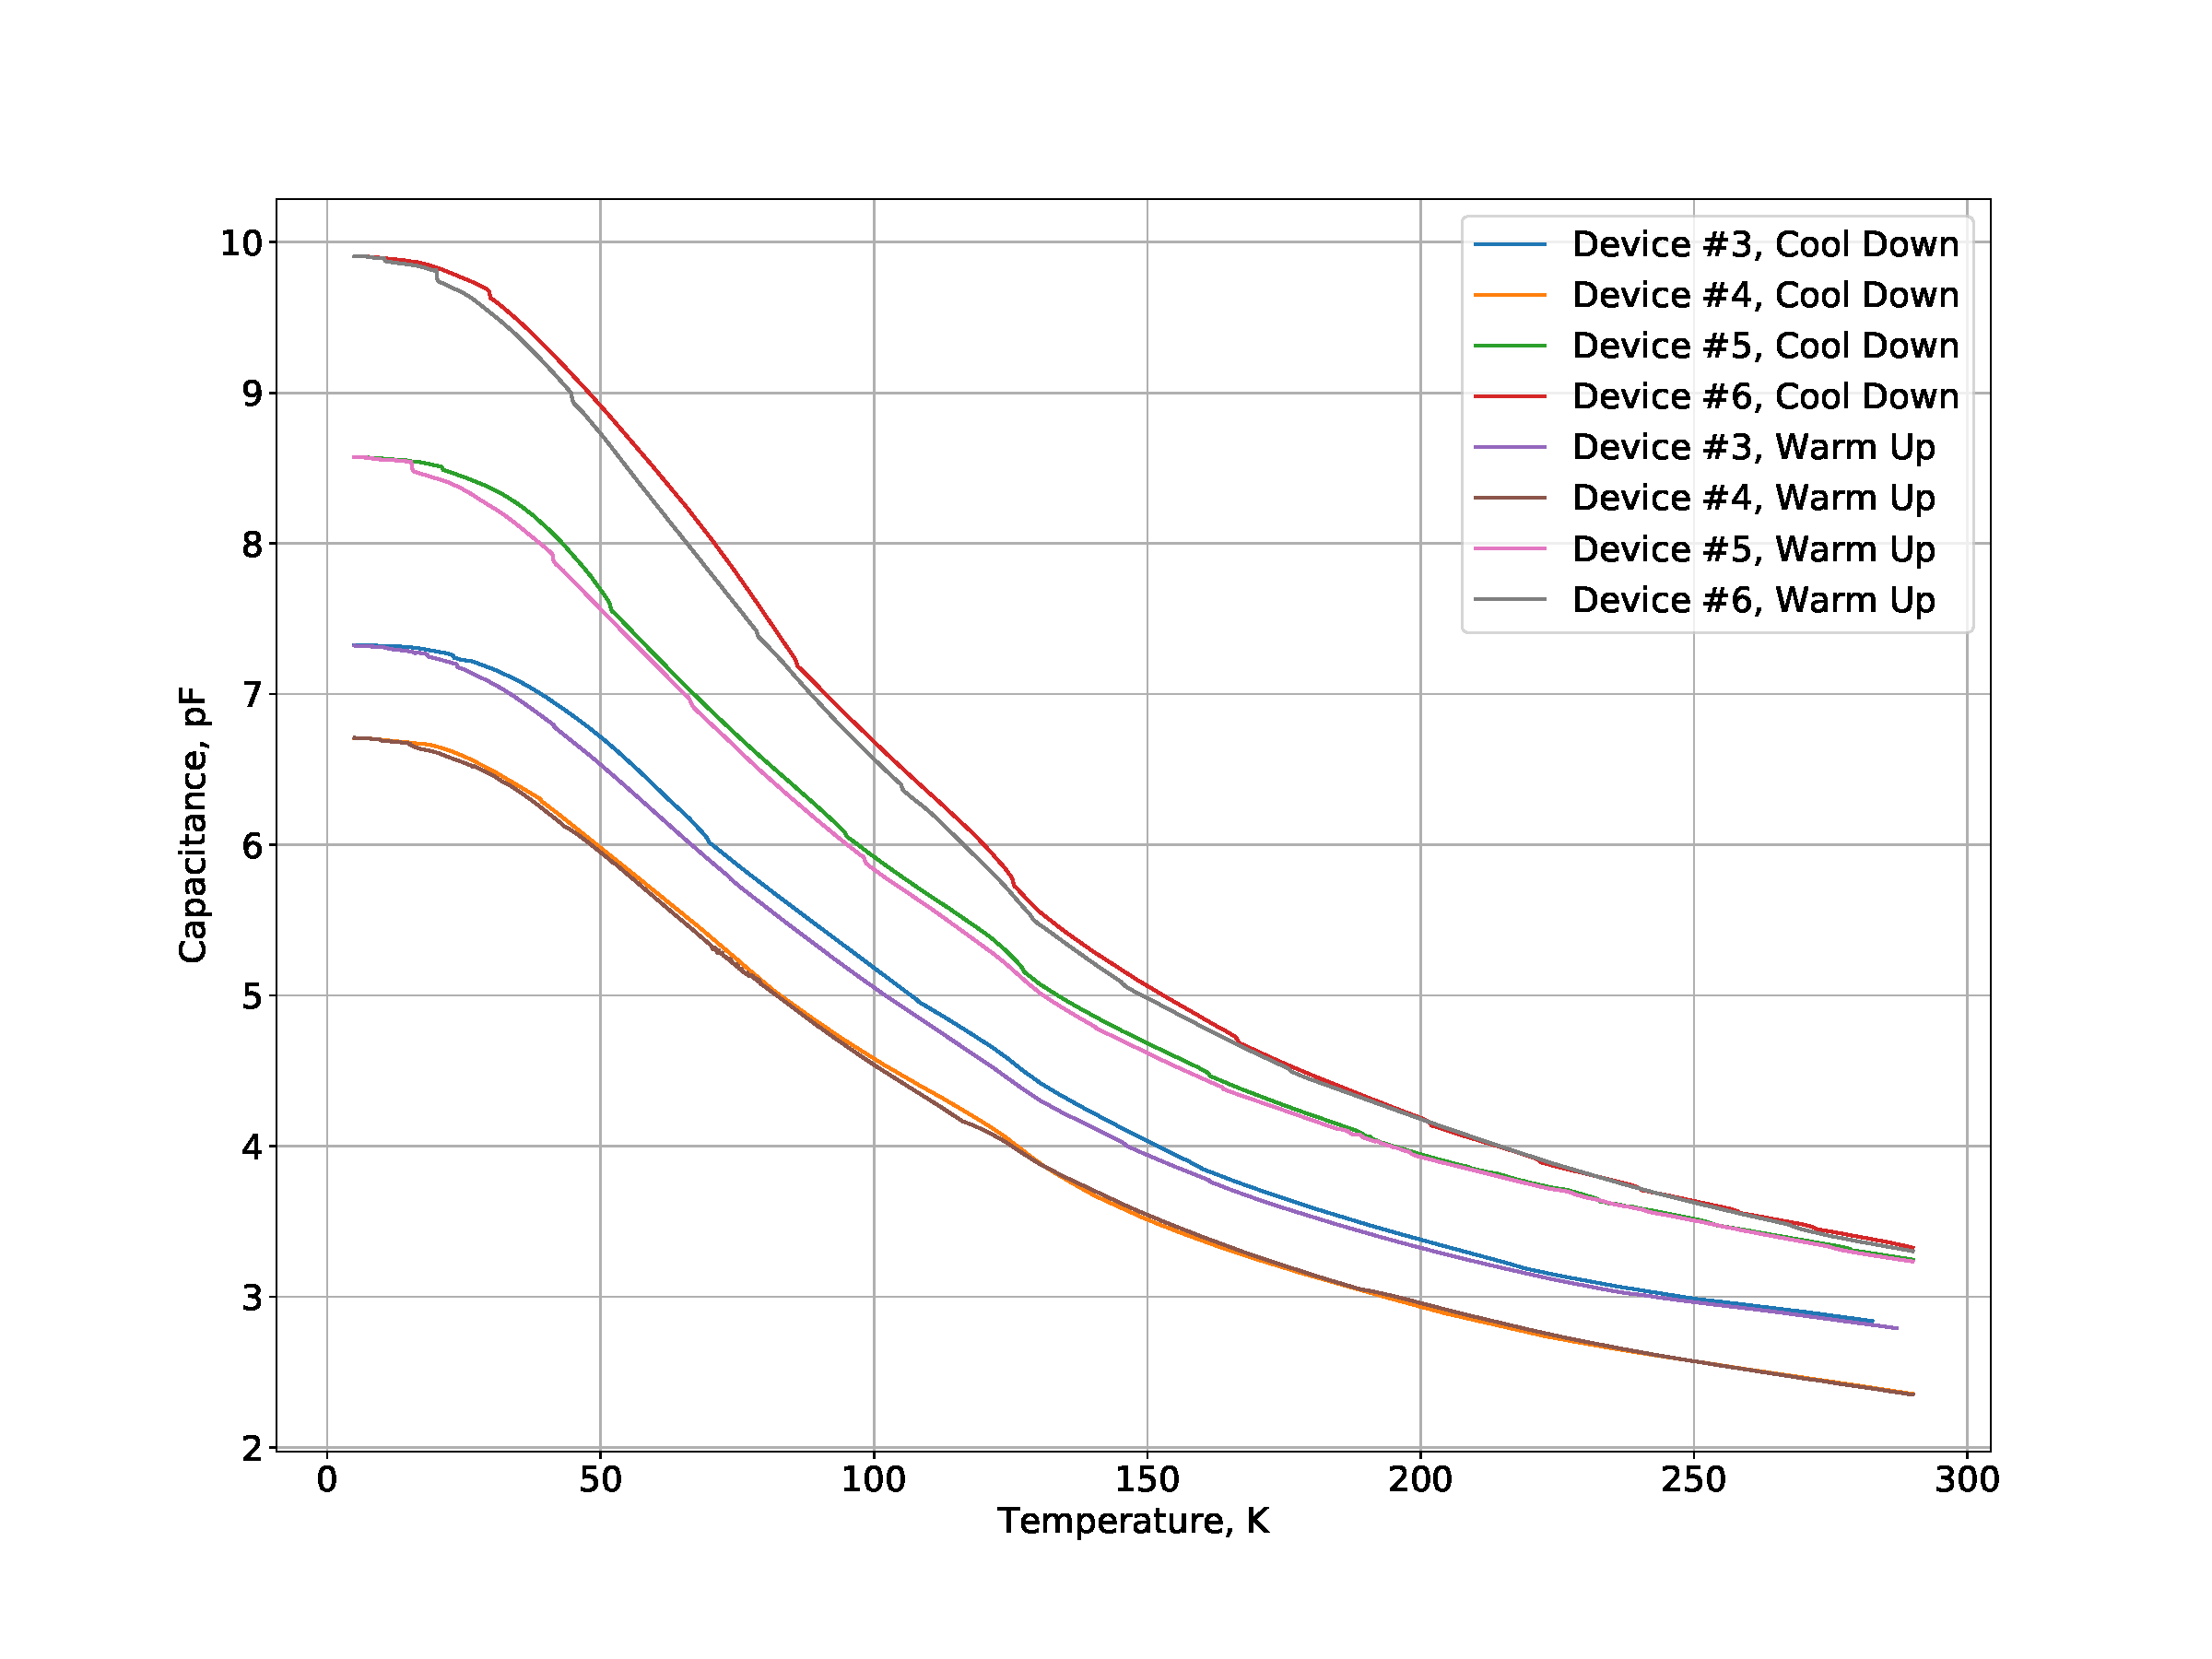
\includegraphics[width=0.9\columnwidth]{figures/annealed_sto_c_vs_t.pdf}
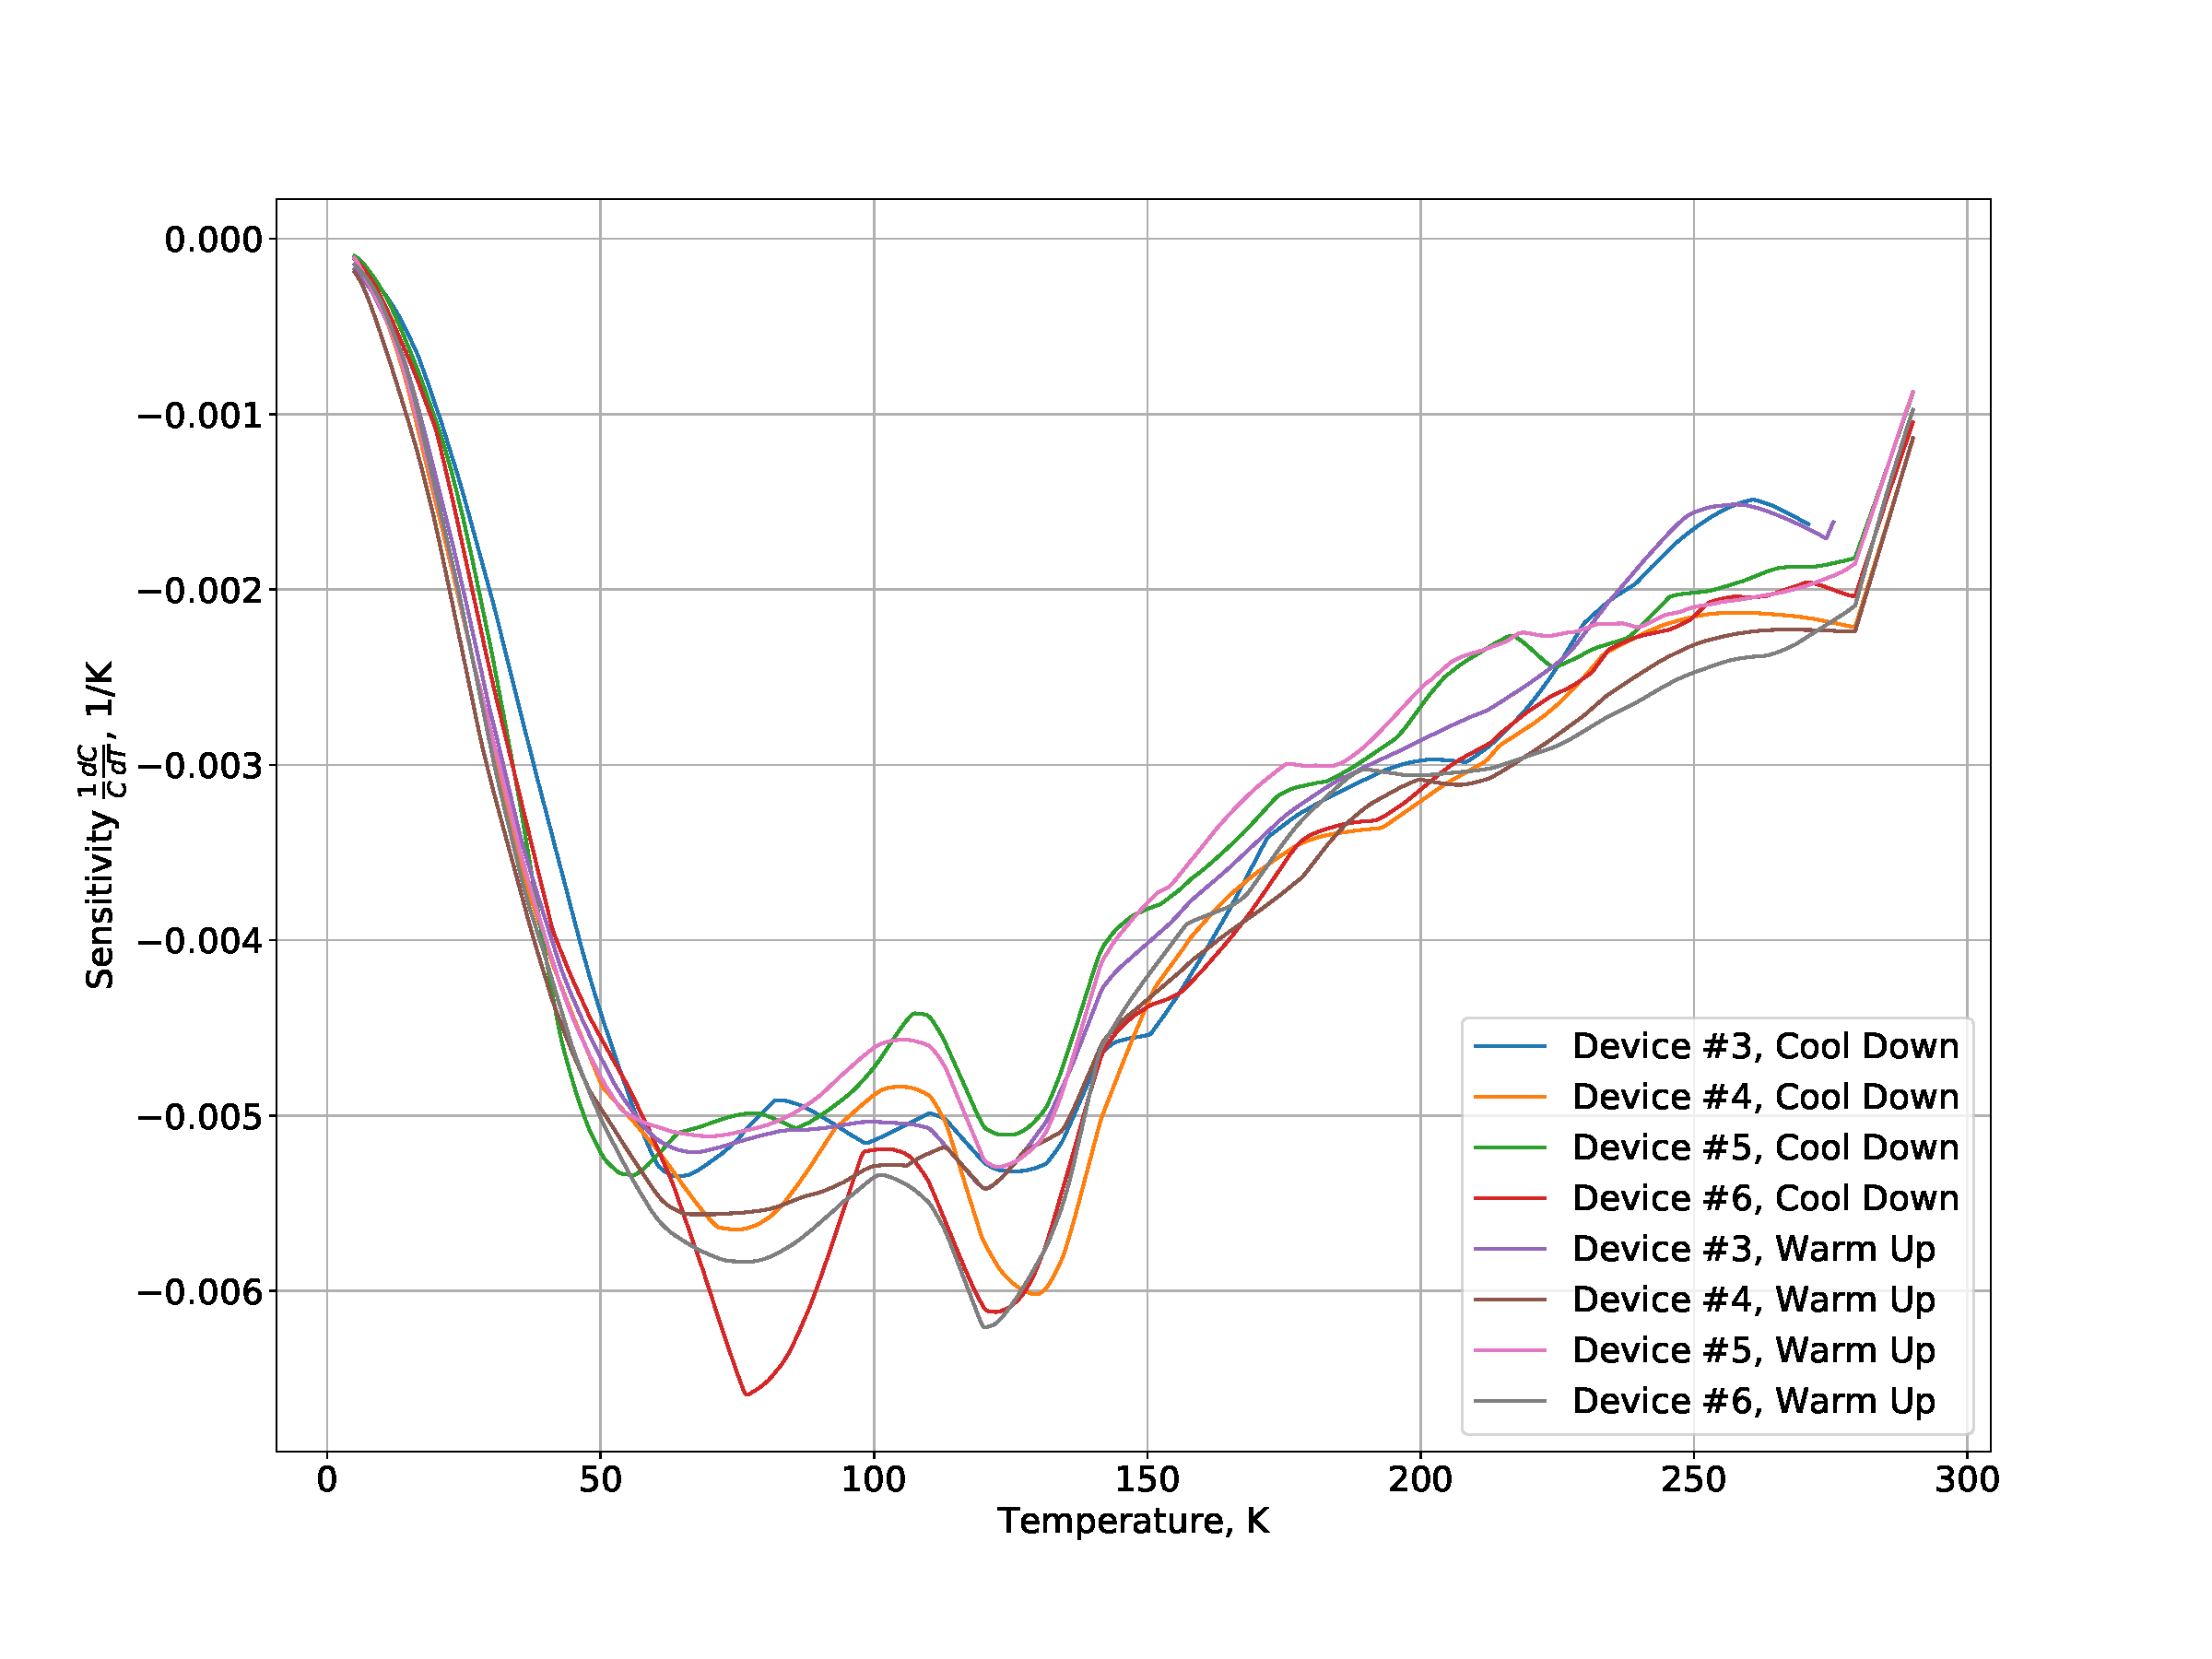
\includegraphics[width=0.9\columnwidth]{figures/annealed_sto_sens_vs_t.pdf}
\end{figure}

\begin{figure} \caption[Annealed STO thermometer dissipation]{Top: Dissipation for the annealed STO devices. Unlike
	the unannealed devices, the dissipation does not increase at low
temperature. Bottom: Heat capacity measurement of a strontium titanate wafer
(blue dots), measured using the Quantum Design PPMS. The measurement does not
show any power law behavior indicative of a phase transition, and so it has not
been doped into the ferroelectric regime. The cubic fit (orange line) is
indicative of simple insulating behavior.}
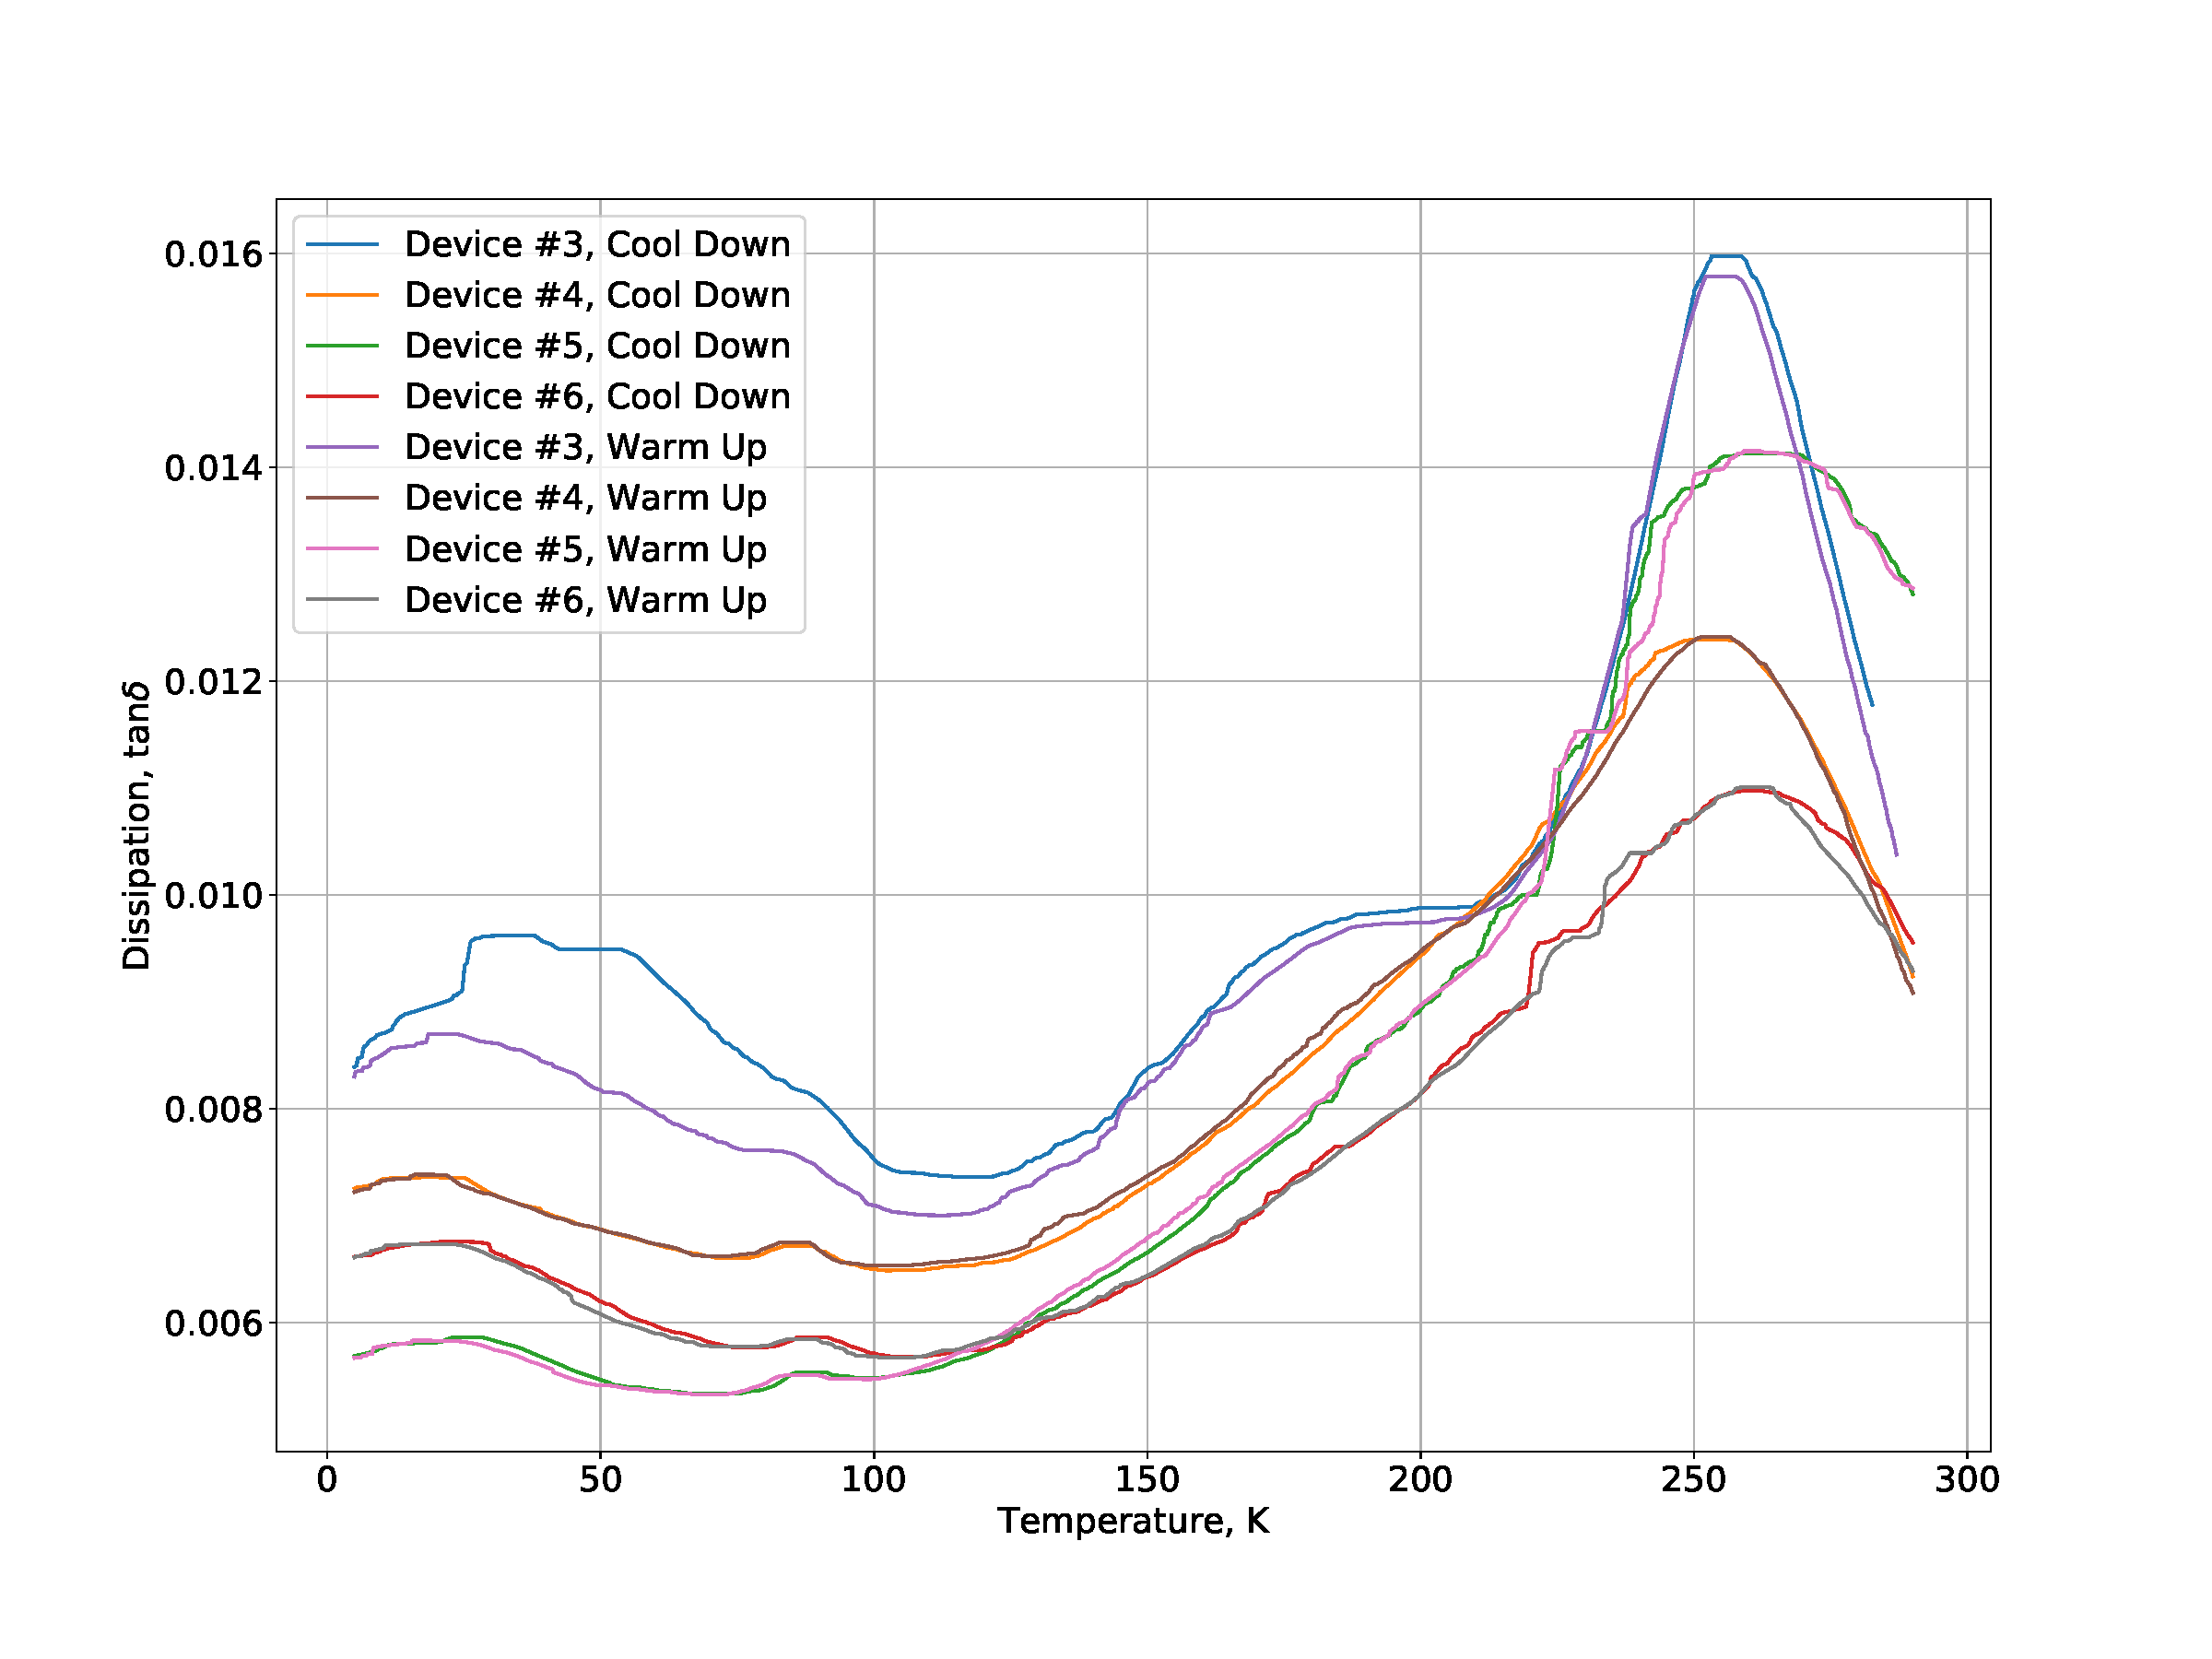
\includegraphics[width=0.9\columnwidth]{figures/annealed_sto_diss_vs_t.pdf}
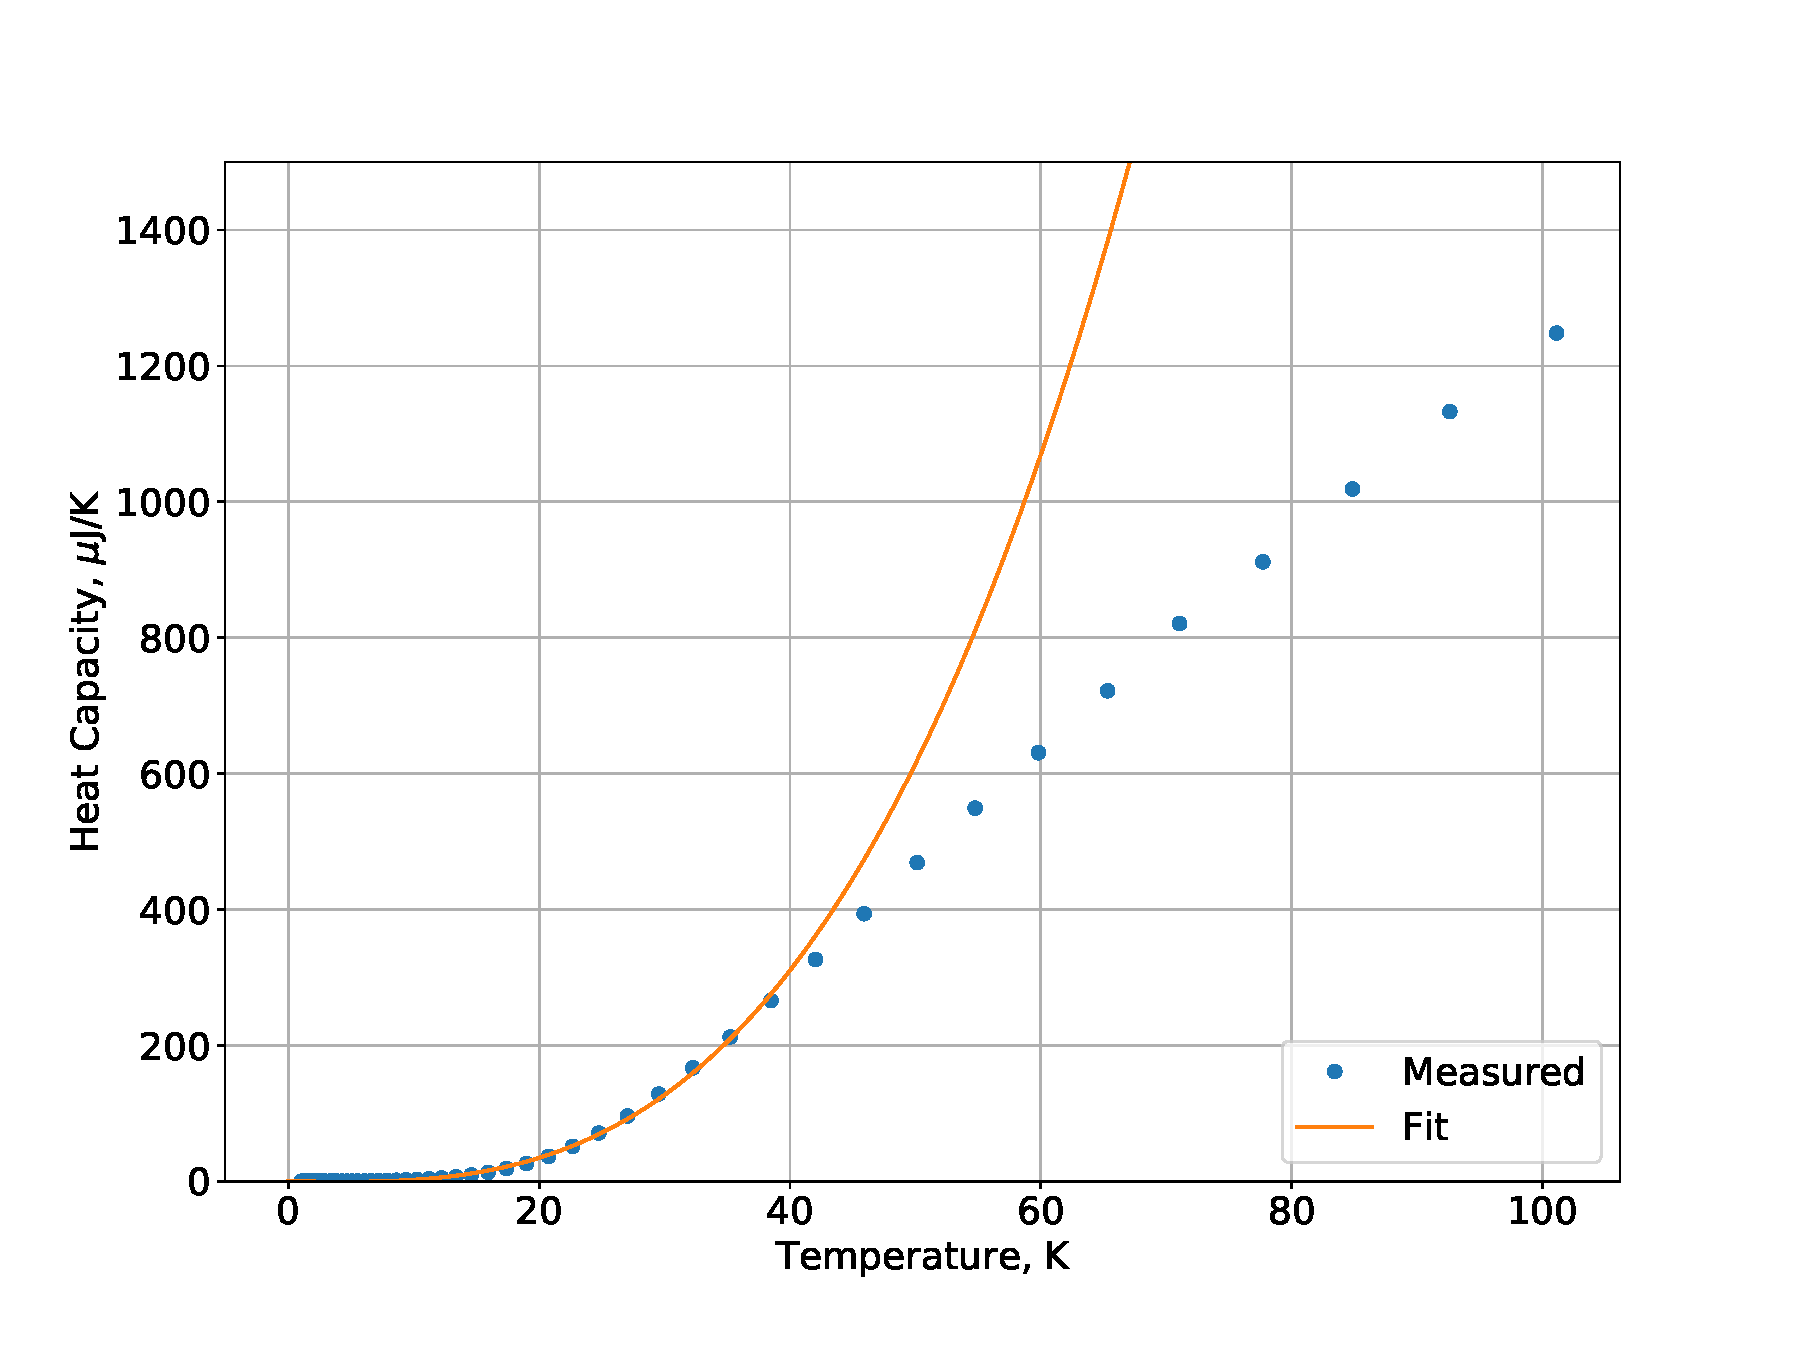
\includegraphics[width=0.9\columnwidth]{figures/annealed_sto_heatcap_vs_t.pdf}
\end{figure}

\begin{figure} \caption[Field response of an annealed STO thermometer]{Relative change in capacitance of an annealed STO
	thermometer in an applied magnetic field, measured up to 14 tesla in
the Quantum Design PPMS. The improved sample mounting in the PPMS eliminates
the background from the flexing of the wires.}
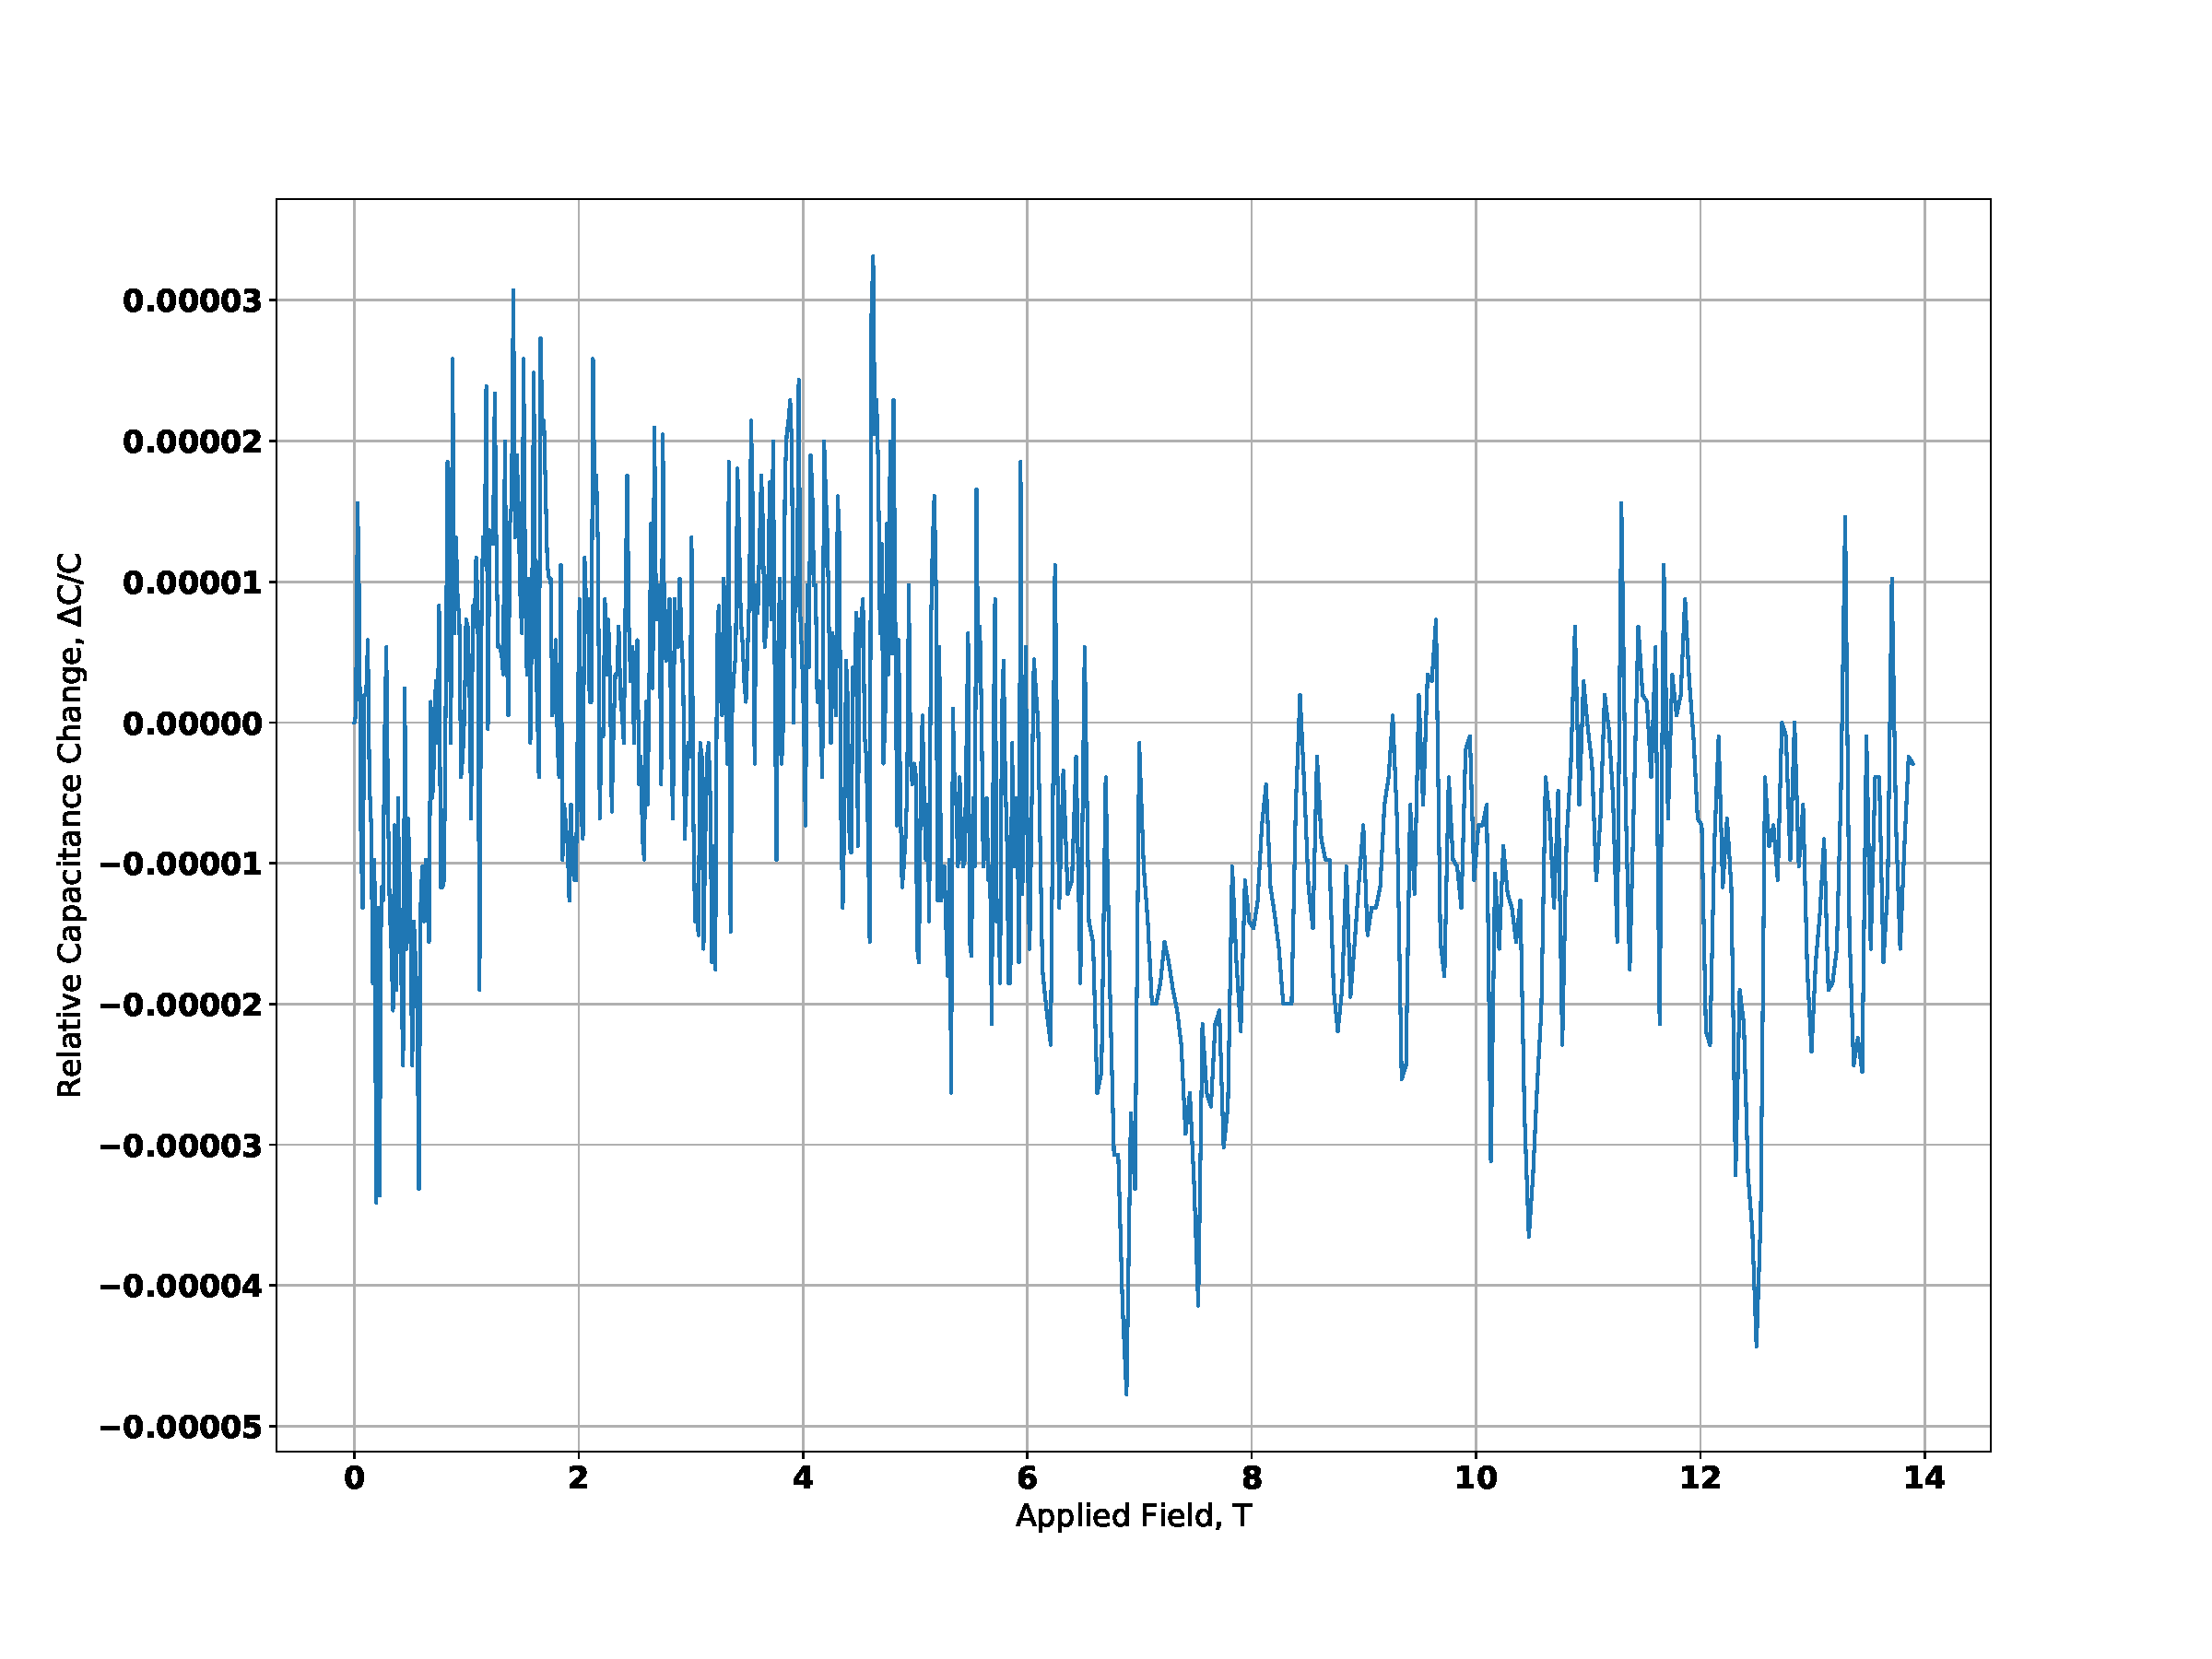
\includegraphics[width=\columnwidth]{figures/annealed_sto_dc_vs_b.pdf}
\end{figure}
	
\chapter{Thermal Measurements of Strontium Copper Borate}

\section{The Shastry-Sutherland Model}
For the above portion of this work, we have mostly talked about thermal measurments of metals. This is a subject which has been studied for many decades at the point. In recent years, there has developed an interest in making thermal measurements on a class of magnetic materials whose properties derive from the geometry of their lattice structures: frustrated magnets. Consider a square lattice of spin-1/2 sites, with antiferromagnetic coupling, i.e. with a Hamiltonian given by
\[ H = J \sum_{\mathrm{n.n.}} s_i \cdot s_j\]
where the sum is over pairs of nearest-neighbor sites, and J is positive. Each $s_i$ can take the value $1$ or $-1$, or alternatively spin up or spin down. We will say that a particular bond between two sites is ``satisfied'' if the sites take values which minimize the energy, which in this case implies they have opposite spins. In the case of a square lattice, we can minimize the total energy by simply fixing one of the sites (e.g. $s_i = 1$), fixing its neighbors with the opposite spin, and repeating this process until every spin is determined. This process will determine the spin at each site unambiguously (up to our initial choice for the first site).
\begin{figure}
	\centering
	\caption[Frustration]{A simple example of frustration in a spin system. If the spins (gray circles) are antiferromagnetically coupled, all of the bonds cannot be satisfied simultaneously. This, this arrangement of spins has no unique ground state.}
	\label{fig:frustration}
	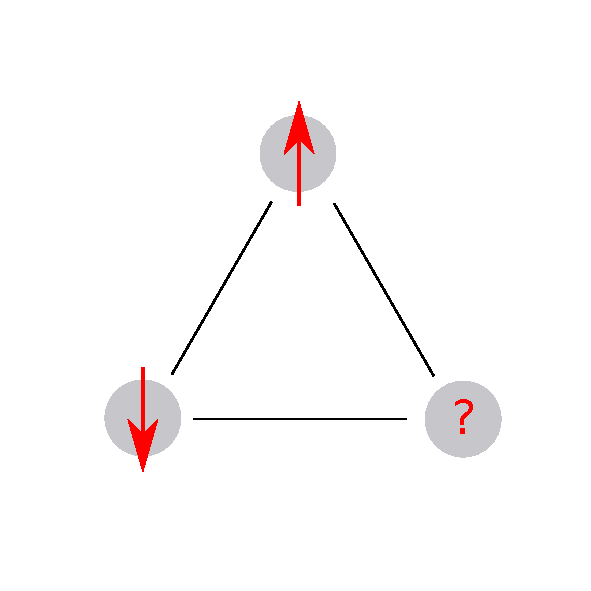
\includegraphics[width=0.6\columnwidth]{figures/frustration.pdf}
\end{figure}

This process does not always work for a general lattice, however. For a simple example, apply the above spin Hamiltonian to the triangle of sites depicted in figure \ref{fig:frustration}. Say we fix the top spin to be up. We can satisfy the bond with the site on the lower left by making it down. But what about the site on the lower right? If we make it spin down, the bond with the spin on the lower left won't be satisfied. If we make it spin up, then the bond with the top spin won't be satisfied. Indeed, for the $2^3 = 8$ possible arrangments of spins on this triangle, six of them have energy $-J$ (the other two, which have all the spins in the same direction, have energy $3J$). This is the essence of frustration: the geometry of the lattice interferes with the formation of long range order.

There has been a great deal of theoretical and experimental research conducted on materials with this sort of frustration. There are many examples of materials with lattice structures involving triangular or tetrahedral elements, and frustration in such materials has the potential to create quite exotic magnetic phases. Since these materials are generally insulators, but may have magnetic excitations that don't carry charge such as magnons, thermal measurements such as the thermal Hall effect are an important tool for studying these phases experimentally. One example are so called spin ices in pyrochlore systems such as Lu$_2$V$_2$O$_7$~\cite{Onose2010} and Tb$_2$Ti$_2$O$_7$~\cite{Hirschberger2015}. The pyrochlore lattice is made up of a series of interconnected tetrahedra. The term spin ice derives from the nonzero entropy in these systems due to the frustration which is analogous to a well known structural frustration in water ice~\cite{Giauque1936}. Both of these materials have relatively large thermal Hall effects considering they are insulators. Another class of materials of great interest are quantum spin liquids~\cite{Anderson1973}. In these materials, frustration prevents the formation of any magnetic ordering at low temperature, resulting in a state with many exotic properties, such as fractional excitations and long range quantum entanglement. Due to the potential for such an exotic phase of matter, there as been intense experimental investigation of spin liquid candidates. Many of these are kagome antiferromagnets, for example herbertsmithite (ZnCu$_3$(OH)$_6$Cl$_2$)~\cite{Asaba2014}. ``Kagome'' refers to the crystal structure of these materials which resembles a particular type of Japanese basket. There has been theoretical~\cite{Owerre2017} and experiemental~\cite{Doki2018} investigation of the thermal Hall effect of these materials. Thermal Hall measurements of spin liquid candidates with hexagonal lattice structures have been performed as well~\cite{Kasahara2018}. The field of quantum spin liquids is quite active and bears much more discussion than I have presented here, but suffice it to say there is much the thermal Hall effect techniques presented in this work have to offer in experimental studies of these facinating materials.

\begin{figure}
	\caption[The Shastry-Sutherland lattice]{Schematic of the Shastry-Sutherland lattice. Each red circle has spin 1/2. The nearest-neighbor coupling $J$ is represented by the solid lines, and the intra-dimer coupling $J_D$ is represented by the dashed line. Each spin is in exactly one dimer.}
	\label{fig:shastry-sutherland}
	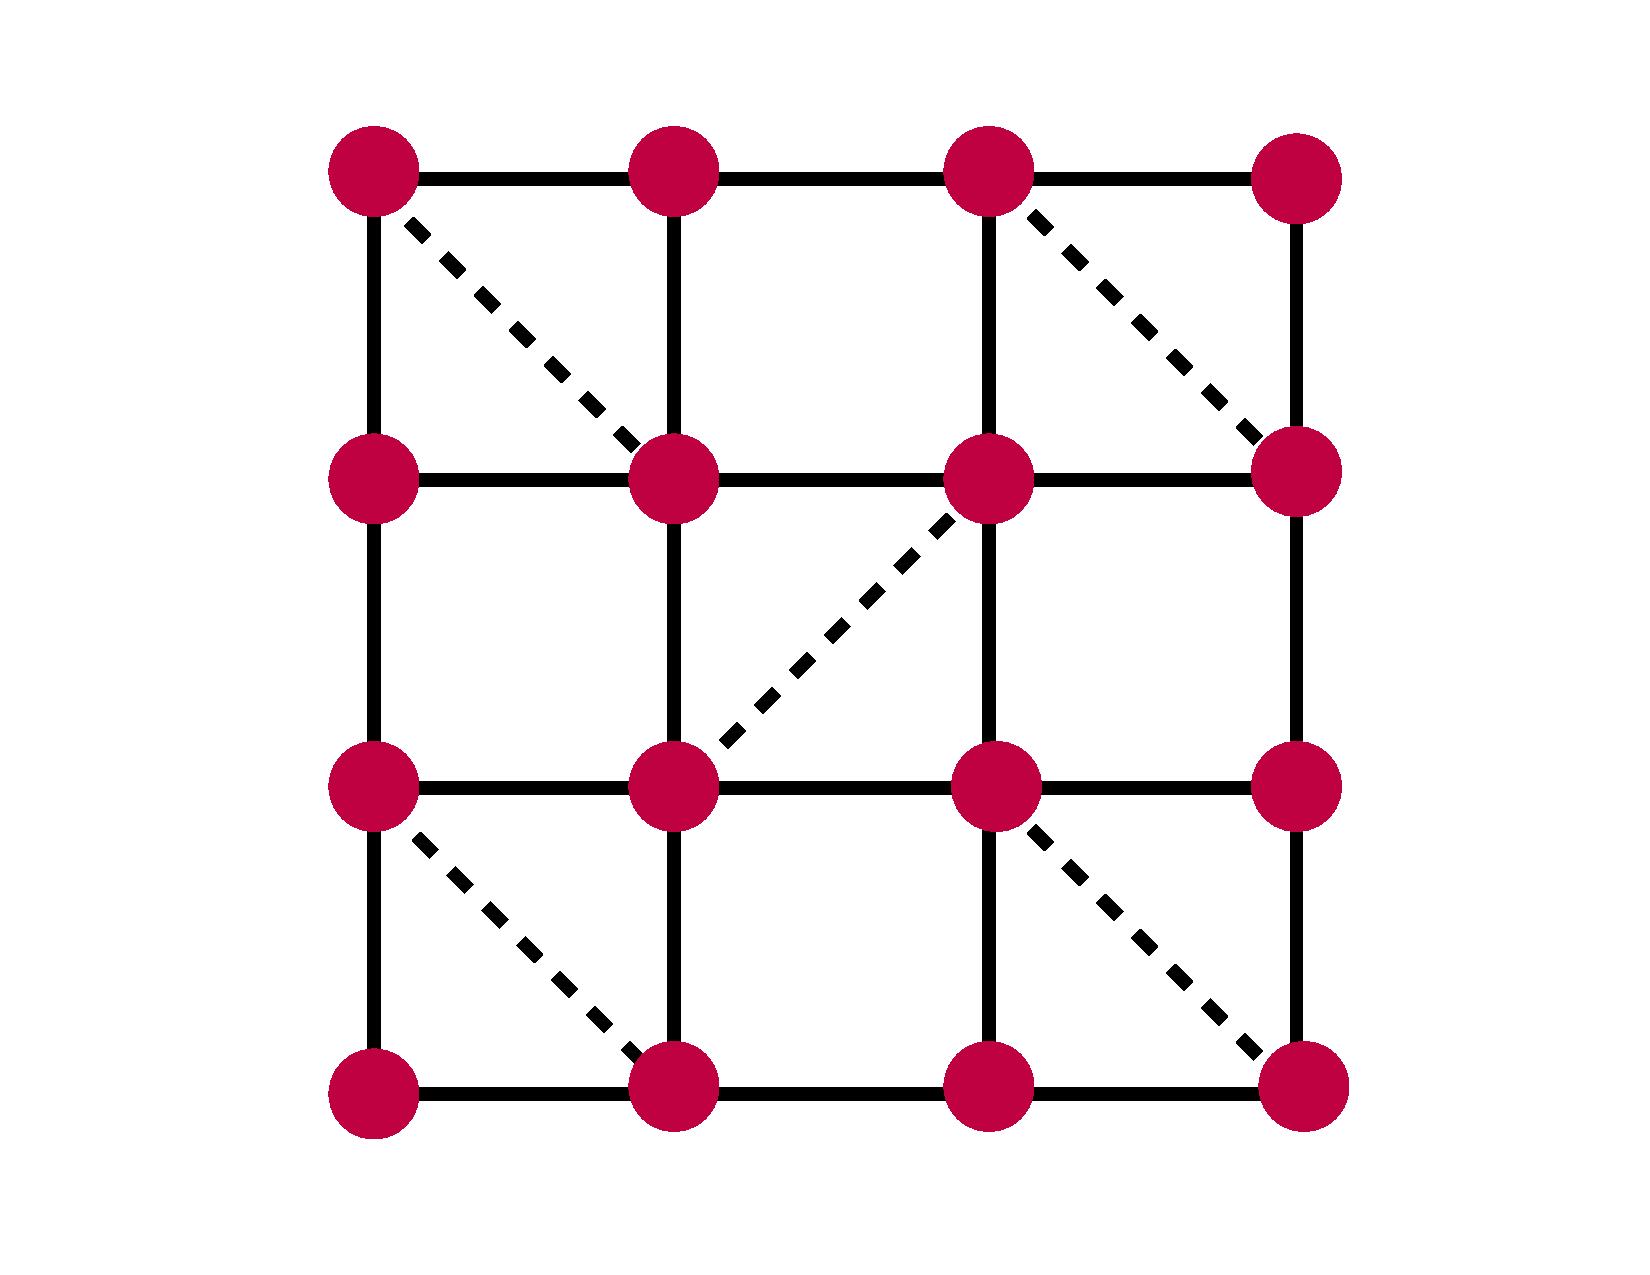
\includegraphics[width=\columnwidth]{figures/ss-model.pdf}
\end{figure}

The above discussion might lead one to believe that frustration can only occur in materials with lattices based on triangles or tetrahedra. Certianly most of the compounds of experimental interest are, but one can introduce frustration to a square lattice by adding interactions across the diagonals. There are potentially many different ways of doing this, but the one we will be interested in is depected in figure \ref{fig:shastry-sutherland}. This model is known as the Shastry-Sutherland model~\cite{Kageyama2005}. In it, each spin is paired across a diagonal with exactly one other spin. The spin Hamiltonian is given by
\[H = J \sum_{\mathrm{n.n.}}s_i \cdot s_j + J_D\sum_{\mathrm{diag}}s_i \cdot s_j\]
where the coupling $J$ is between nearest neighbors on the square lattice (solid in the figure) and $J_D$ is between the diagonals (dashed in the figure). The ground state of this Hamiltonian of course depends on the relative values of $J$ and $J_D$, but there are two cases we can consider intuitively. If $J$ is much stronger than $J_D$, we effectively have the square lattice antiferromagnet again. The more interesting case is when $J_D$ dominates over $J$: each pair of spins connected by a diagonal hybridizes to form a singlet state give by
\[ | s \rangle = \frac{1}{\sqrt{2}}(|\uparrow \downarrow \rangle - | \downarrow \uparrow \rangle) \]
with the full ground state being a direct product of these singlets. The odd pairity of the singlet state with respect to exchange of the spins in each dimer actually ensures that the $J$ term does not contribute to the energy at all~\cite{Miyahara1999}. 

Each individual dimer also has excited states given by the three triplets:
\begin{align*}
	| t_1 \rangle &= | \uparrow \uparrow \rangle \\ 
	| t_0 \rangle &= \frac{1}{\sqrt{2}} (| \uparrow \downarrow \rangle + | \downarrow \uparrow \rangle) \\
	| t_{-1} \rangle &= | \downarrow \downarrow \rangle
\end{align*}
These triplets all have even parity with respect to exchange of the spins within the dimers, so one might expect that they would have strong dispersion. Actually, the triplets are highly localized, and this is a result of the frustration in the lattice~\cite{Kageyama2005}. Specifically, each spin in a dimer is connected to each of its neighboring spins in a triangle formed with two $J$ couplings and one $J_D$ coupling. Thus despite the strong interactions between the dimers, the triplet states are completely dispersionless in this model.

\begin{figure}
	\caption[Crystal structure of strontium copper borate]{(a): Crystal structure of Strontium Copper Borate, with the $c$ axis out of the page. The copper atoms (copper colored) make up the Shastry-Sutherland lattice. The strontium atoms (green) are set back into the page by half a unit cell. Image generated using Jmol~\cite{jmol}. (b) through (d): Diagram demonstrating the equivalence of the crystal structure of SCBO to the Shastry-Sutherland lattice. To go from the SCBO lattice to the Shastry Sutherland lattice, we elongate the distance between the dimer pairs until the diamond shape containing them has been turned into a square. Reproduced from~\cite{Kageyama2005}.}
	\label{fig:scbo_crystal}
	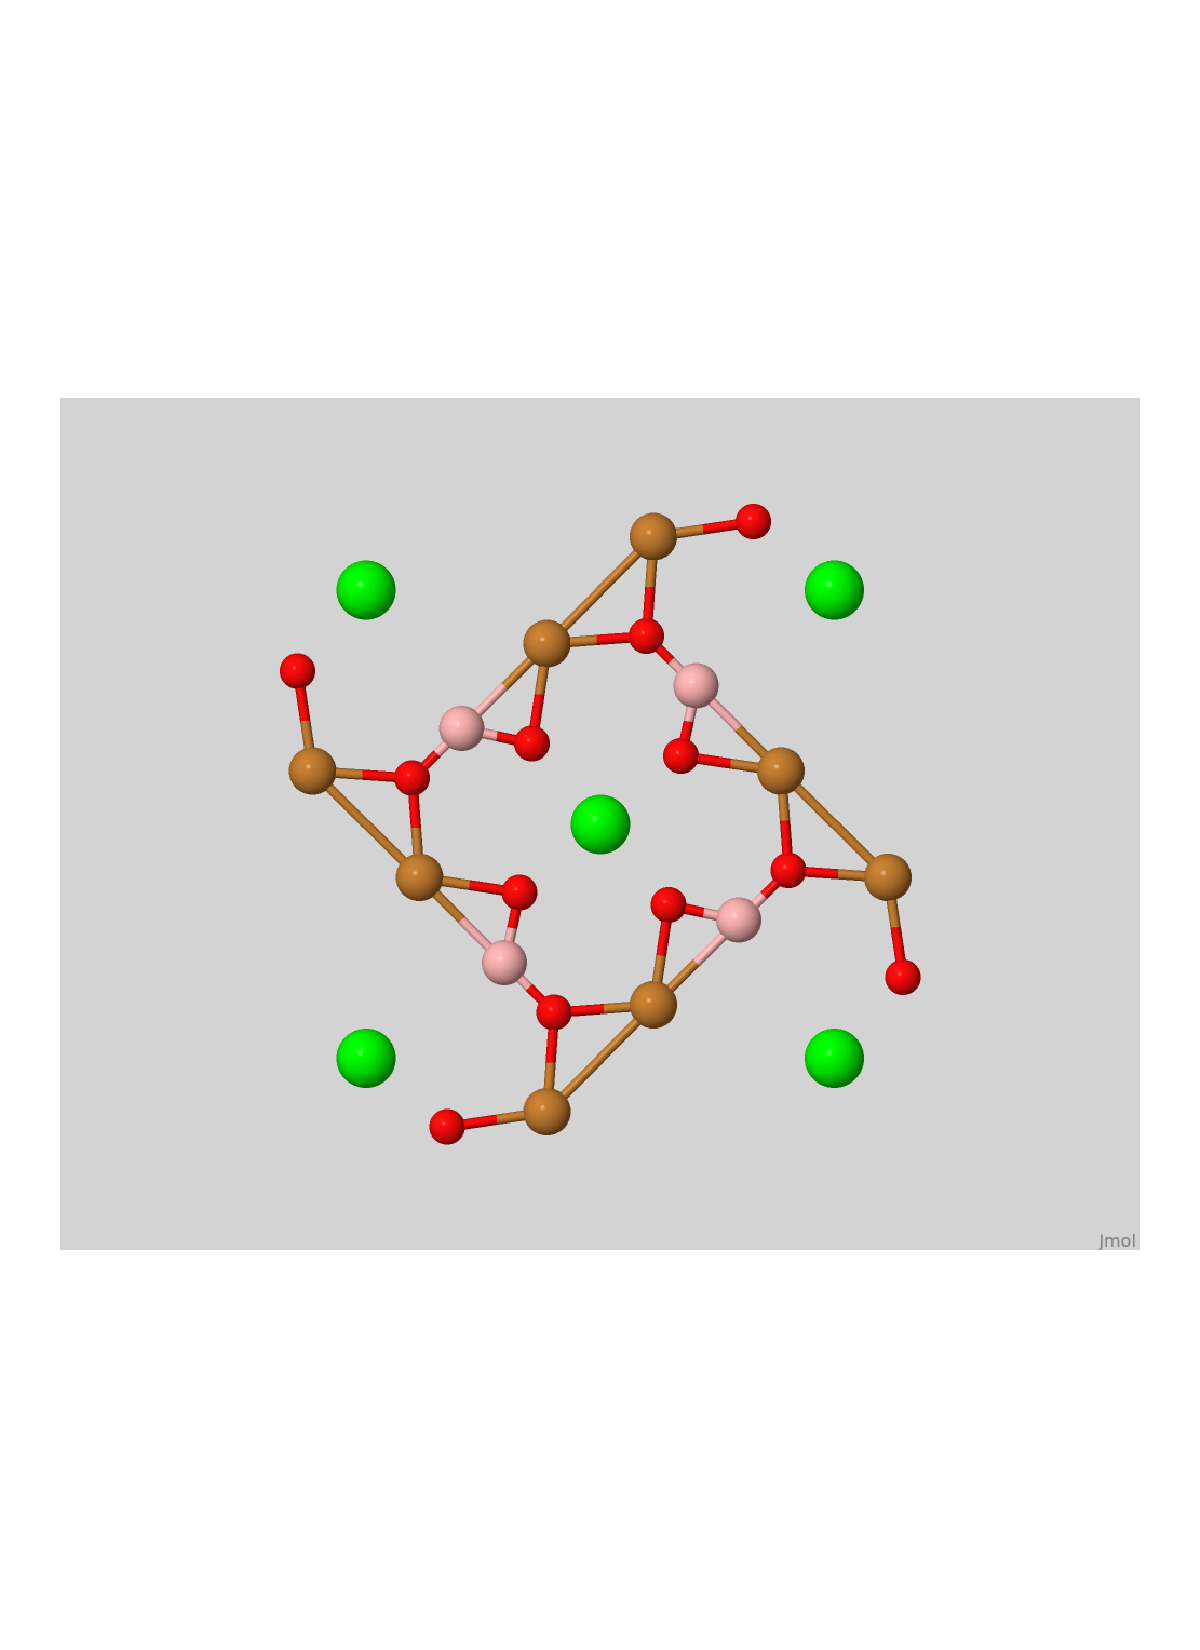
\includegraphics[width=\columnwidth,trim={0 2.5in 0 2.5in},clip]{figures/scbo.pdf}
	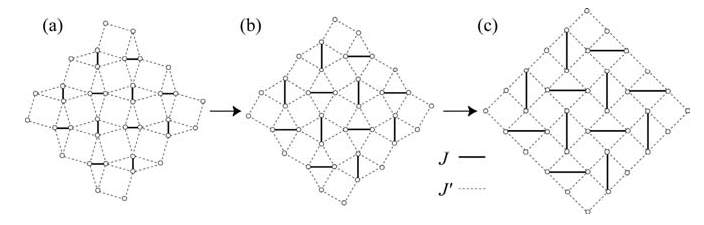
\includegraphics[width=\columnwidth]{figures/scbo_to_ss_kageyama.pdf}
\end{figure}

Facinating as this model is, it is not of much experiemental interest unless it can be realized as an actual material. There are some clear difficulties with this in principle, particularly if we are interesting in the dimer ground state. Monte carlo simulations have shown that in order to get this phase, we must have $J/J_D < 0.7$, i.e. the intradimer coupling must be stronger than the interdimer coupling by a few tens of percent~\cite{Miyahara1999}. If the lattice looked like that depicted in figure \ref{fig:shastry-sutherland}, each atom would need to be more strongly coupled to an atom diagonal from it than from it's nearest neighbor! There is, it turns out, one material which can be modeled by the Shastry-Sutherland Hamiltonian, and that is SrCu$_2$(BO$_3$)$_2$ (Strontium Copper Borate, commonly abreviated SCBO). Figure \ref{fig:scbo_crystal} shows it's crystal structure, which at first glance bares little resemblence to the Shastry-Sutherland lattice. It is, however topologically equivalent: the squares in the Shastry-Sutherland lattice have been turned into diamond shapes, with the short axis corresponding to the dimer pair. Thus, the intradimer coupling $J_D$ can plausibly be stronger than the interdimer coupling $J$. 

\begin{figure}
	\caption[Magnetic moment of a SCBO sample]{Magnetic moment of a Strontium Copper Borate sample, taken at 1 T. The behavior is indicative of the triplon spin gap.}
	\label{fig:scbo_magmom}
	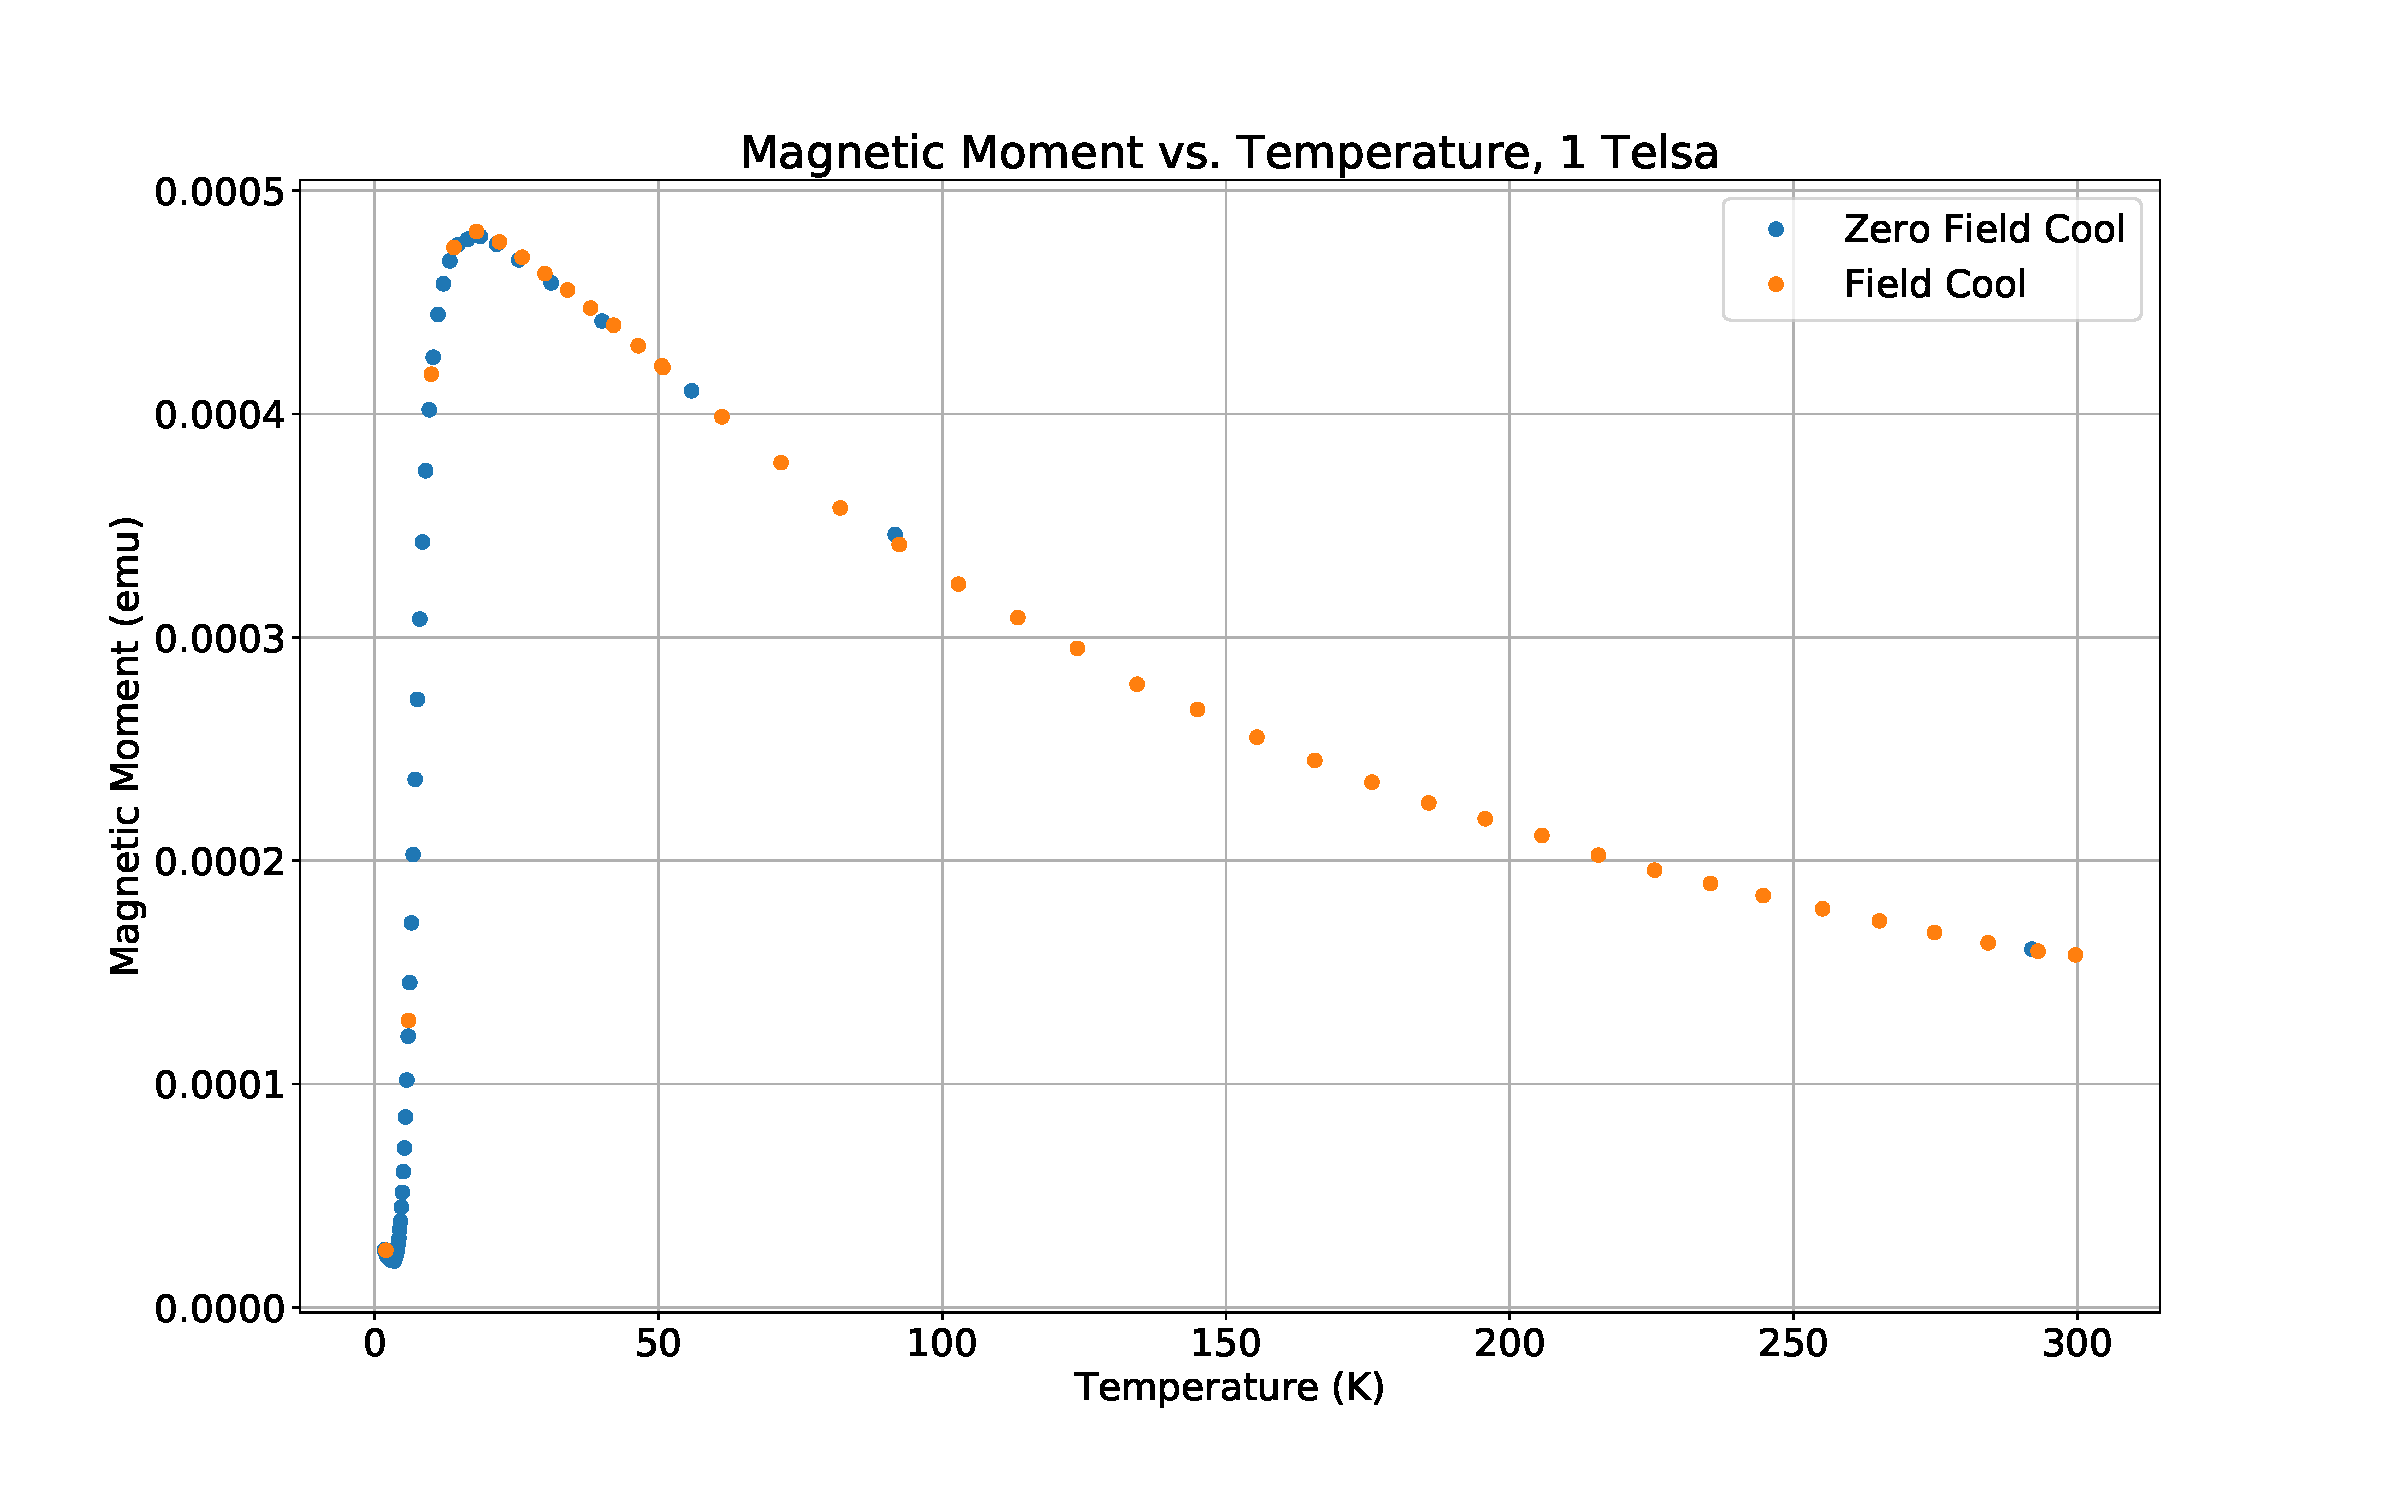
\includegraphics[width=\columnwidth]{figures/SCBO_m_vs_t.pdf}
\end{figure}

What experimental evidence exists that the ground state of SCBO looks like the direct product of singlets described above? One simple way of checking is by measuring the magnetic susceptibility. Figure \ref{fig:scbo_magmom} shows the magnetic moment of a sample of SCBO as a function of temperature with an applied field of 1 T, measured using the Vibrating Sample Magnetometer in our Dynacool PPMS system. At high temperatures, the dependence looks qualitatively like Curie-Weiss $1/T$ behavior. However, the magnetic moment drops precipitously at low temperature, indicating the opening of a spin gap. This is consistent with what was described above: The singlet states contribute no net magnetic moment, but the $|t_1\rangle$ and $|t_{-1}\rangle$ triplet excited states do. At low temperatures, these excitations are frozen out. Work by others has used this data to fit for the coupling constants, finding $J/J_D = 0.635$ and $J = 85$K \cite{Miyahara2000}. This puts SCBO barely into the dimer phase, and corresponds to a spin gap of 35 K. Additionally, by measuring the sample in both field-cooled and zero-field-cooled configuration, we can see there is no hysteresis indicating the formation of some other magnetic ordering. Thus we are confident the samples of SCBO actually have a ground state similar to that describe above.

In the discussion of the Shastry-Sutherland model above, it was noted that the frustration of the lattice resulted in the triplet states being totally dispersionless. Perhaps this makes sense for a toy model, but in an actual material one would expect some second order effect to introduce some dispersion. This is indeed the case in SCBO, and these mobile triplet states are termed ``triplons''. The next section will discuss these lower order effects, and the significant implications they have for thermal measurements in SCBO.

\section{Strontium Copper Borate as a Bosonic Topological Insulator}

In order to induce dispersion in the triplon modes in SCBO, we must have an interaction which is not supressed by the lattice frustration. The simplest way of doing this is by introducing a so-called Dzyaloshinsky-Moriya (abbreviated DM) interaction:
\[ H_{\mathrm{DM}} = \sum_{\mathrm{n.n.}} \mathbf{D} \cdot (s_i \times s_j) \]
The strength of this interaction is characterized by the vector $\mathbf{D}$. This interaction can act both between pairs of spins in a dimer and between the dimers themselves. This results in a full Hamiltonian (including an applied magnetic field $h_z$):
\[ H = J_D \sum_{\mathrm{n.n.}} s_i \cdot s_j + J \sum_{\mathrm{n.n.n}} s_i \cdot s_j + \sum_{\mathrm{n.n.}} \mathbf{D}_D \cdot (s_i \times s_j) + \sum_{\mathrm{n.n.n.}} \mathbf{D} \cdot (s_i \times s_j) - g_z h_z \sum_i s_i^z\]
In this Hamiltonian, ``nearest neighbor'' refers to the coupling between two spins in the same dimer, and ``next nearest neighbor'' referst to the coupling between dimers. This is correct when refering to the lattice structure of SCBO, but is the opposite for the Shastry-Sutherland model (see figure \ref{fig:scbo_crystal} and the Shastry-Sutherland Hamiltonian from above, where the ``nearest neighbors'' are along the square lattice, and not within the dimers, as they are in SCBO). The symmetry of the lattice under exchange within the dimers $\mathbf{D}_D$ means that only one component can be nonzero, whereas the interdimer coupling $\mathbf{D}$ can have all three components~\cite{McClarty2017}. Figure \ref{fig:scbo_triplon_bands} shows these bands imaged using neutron scattering. The top row shows the experimental data, and the bottom row shows theoretical computations of the bands with the coupling strengths determined using the data. Contrary to the prediction from the Shastry-Sutherland model without the DM interaction, the triplons do not have a totally flat dispersion, and show some spliting without any applied field. The antisymmetry of the DM terms in the Hamiltonian make it compatable with the frustration in the lattice, and so allow the triplons to disperse. This is despite the fact that the DM interaction is small compared to the higher-order effects, the above work found the largest component of $\mathrm{D}$ was about 3\% as large as $J_D$~\cite{McClarty2017}.
\begin{figure}
	\centering
	\caption[Triplon Bands in SCBO]{Triplon band structure, imaged by neutron scattering by~\cite{McClarty2017}, showing dispersion induced by the DM interaction. Experiemental data in top row, theoretical calculatons in the bottom row.}
	\label{fig:scbo_triplon_bands}
	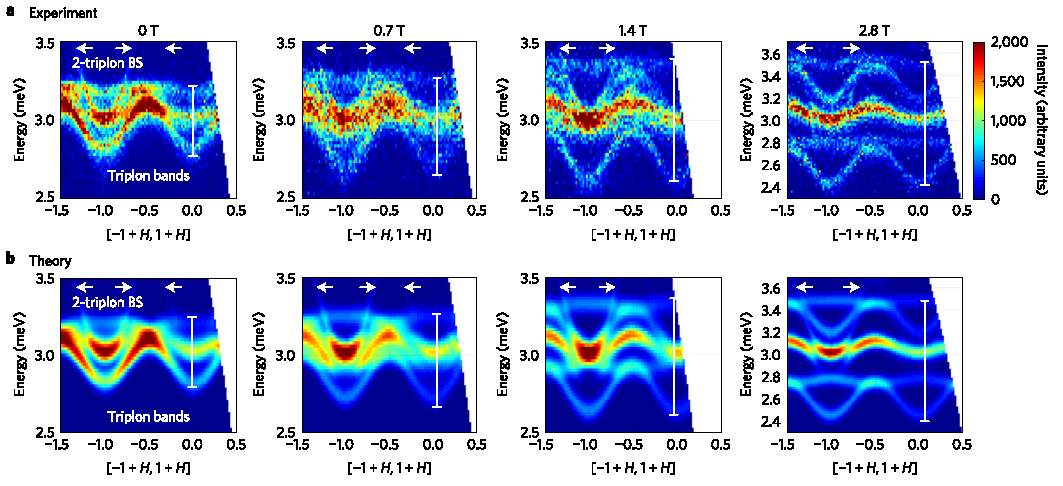
\includegraphics[width=\columnwidth]{figures/SCBO_triplon_bands_McClarty.pdf}
\end{figure}

The signature of the DM interaction in SCBO can be observed without doing neutron scattering by performing heat capacity measurements. Figure \ref{fig:scbo_hc} shows measurements performed on our SCBO samples in our Dynacool PPMS, as well as a comparison to the work done by Jorge et. al.~\cite{Jorge2005}. At zero field, there is an anomaly in the heat capacity at around 7.5K. This anomaly has been attributed to resonant scattering of phonons by triplet excitations with $s^z = 0$~\cite{Hofmann2001}. Once a magnetic field is applied perpendicular to the Shastry-Sutherland plane, this anomaly shifts lower in temperature as the phonons scatter off triplon states with $s^z \neq 0$. However, once the field is increased to about 10 T to 14 T, a new anomaly begins to grow around 3 K. This second anomaly is due to mixing between the states with $s^z = 0$ and those with $s^z \neq 0$. This mixing is acheived through the DM terms in the Hamiltonian, which does not conserve $s^z$. Plots from the paper show reproduced in figure \ref{fig:scbo_hc} show calculations of the heat capacity for data taken in fields above 22 T where the difference is more apparent. This mixing becomes most apparent when the difference in energy between the states with $s^z = \pm 1$ is comparable to $|\mathbf{D}|$, which is why such strong fields are required to generate it. Thus, the effect of the DM interaction can be observed directly in our samples via heat capacity measurements.

\begin{figure}
	\centering
	\caption[Low Temperature Heat Capacity of SCBO]{Top: Field-dependent low temperature heat capacity measurement of Strontium Copper Borate, measured in our Dynacool PPMS system, Plotted as $C/T$ to make the presence of two anomalies more clear. Bottom: Heat Capacity plotted as C/T versus temperature, taken from~\cite{Jorge2005}. The symbols are actual data, and the lines are data computed using a fit for the DM interaction. The dashed line in the lower panel is a calculation where the DM term is ignored.}
	\label{fig:scbo_hc}
	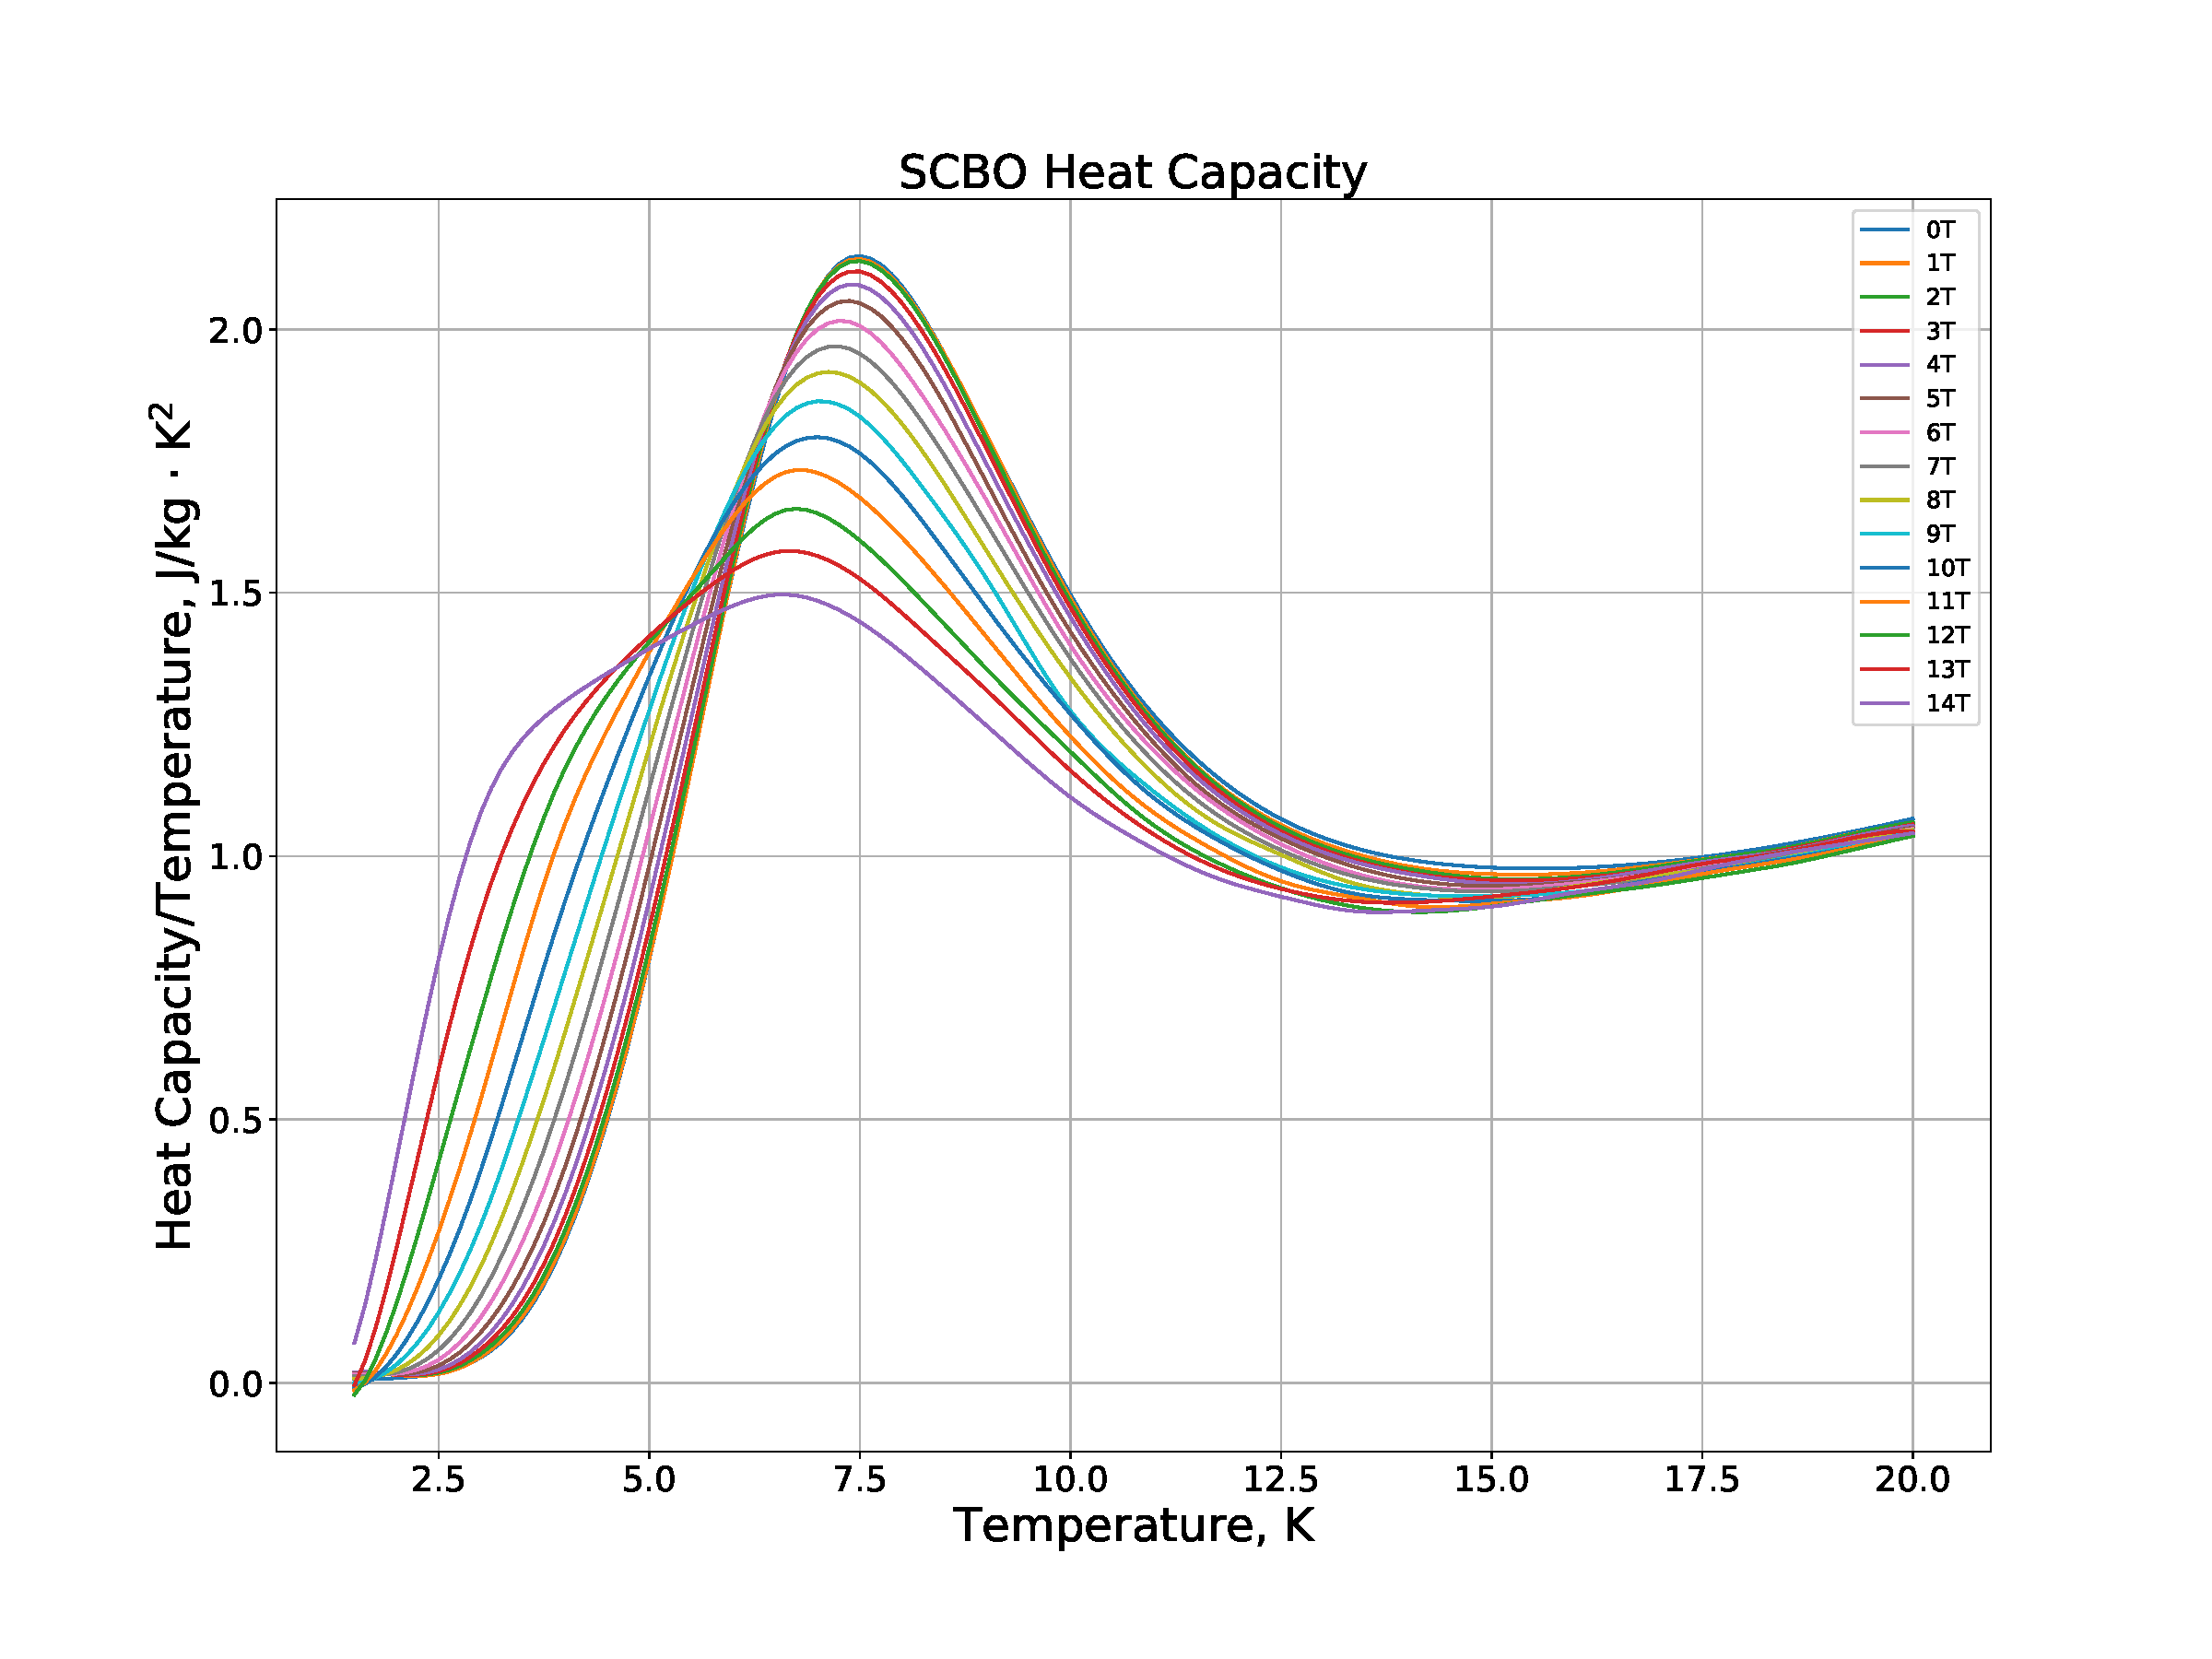
\includegraphics[width=\columnwidth]{figures/SCBO_total_HC_over_T.pdf}
	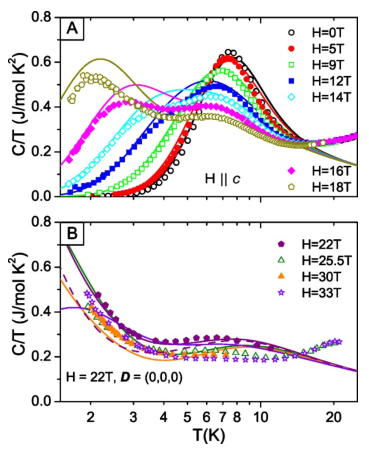
\includegraphics[width=0.5\columnwidth]{figures/SCBO_HC_Jorge_2005.pdf}
\end{figure}

There has been some theoretical work which indicates that the DM interaction has the potential to introduce a new type of physics to this system: triplon bands with nontrivial topology. The importance of band topology has recently opened up an entirely new line of research in condensed matter physics, ever since materials with topologically non-trivial bands were predicted~\cite{Fu2007} and experiementally observed~\cite{Hsieh2008} at the end of the first decade of the 2000s. In mathematics, ``topology'' refers to the study of continuous deformation of geometric objects. ``Continuous deformation'' can intuitively be thought of as transformations which stretches or compresses an object without tearing or puncturing it. Topology is primarily concerned with the properties of such objects which are invariant under continuous deformations~\cite{Munkres}. A commonly cited example is the number of holes in an object: a donut can be continuously molded into a coffee mug, while a sphere cannot be continuously deformed into a dount without puncturing it. Such a quantity is known as a ``topological index''. This particular invariant is sometimes called the ``genus'' of a surface by mathematicians. When the object in question is a (Reimannian) manifold (loosely, an object which looks locally enough like Euclidian space in which one can do calculus, e.g. the surface of a sphere or a torus), it is possible to compute the genus $g$ by integrating local information on the surface, i.e. it's mean Gaussian curvature $K$:
\[ \int_M K dA = 2\pi * (2 - 2 g) \]
This is a specific case of the more general Gauss-Bonnet theorem, which in general connects topological invariants to integrals over local infomation about curvature~\cite{Lee}. Thus, with this local information, we can classify these objects by whether or not they can be continuously deformed to each other.

The significance of this mathematical formalism to condensed matter physics comes through the definition of Berry curvature, which assigns a curvature to a quantum state based on how its quantum phase changes as it is  adiabatically transformed into other states~\cite{Berry1984}. In much the same way that the mean Gaussian curvature can be integrated to find an invariant which classifies which manifolds can be continuously deformed into others, the Berry curvature can be integrated to produce a topological index known as a Chern number. The Chern number thus indexs which states can be adiabatically transformed into each other in the same was as the genus. In the context of a band structure, states in the same band can be adiabatically transformed into each other, and so all states in a band have the same Chern number. Thus, we conventionally assign Chern numbers to bands. Much of the experiemental research on topological bands in condensed matter physics has focused on the topology of electron bands (as opposed to magnon bands such as triplons, for example) in compounds such as bismuth selenide~\cite{Hsieh2008}. Here, one of the most important experiemental features of electron topology can be observed: the existance of topologically protected surface states. Bismuth selenide has an insulating bulk, it's band structure has a gap between two bands with different Chern numbers. However, states of electrons in vacuum outside they crystal have ``trivial'' topology. Thus, at the interface between the crystal and the outside, the gap must close so that the topology of the bands can be unwound. This has the result of creating conducting surface states which span the gap, even though the bulk material is an insulator. These states are ``topologically protected'' in the sense that they are a necissary feature of the interface between bismuth selenide and the vacuum (or some other insulator with trivial topology). If one cuts a crystal of bismuth selenide in half, the surface states will appear on the surface without having to modify it in any way. These surface states have many unique properties, such as Dirac-like dispersion and spin-momentum locking (i. e. the direction of their momentum necissarily determines their spin)\cite{Fu2007}. Because of these properties, finding materials which host these states has been an area of intense focus for the field in general and our lab in particular~\cite{Li2014}.

\begin{figure}
	\centering
	\caption[Chiral Edge Modes in SCBO]{Figures concerning chiral edge modes in SCBO, reproduced from~\cite{Romhanyi2015}. a through e: Schematic of the triplon bands as a function of applied magnetic field perpendicular to the Shastry-Sutherland plane. At fields above zero but below the critical field $h_c$, the upper and lower bands have nonzero Chern number. f and g: Band diagram showing the chiral edge modes in the gap between triplon bands. h through j: Theoretical prediction of thermal Hall conductivity. The component from the chiral edge modes should in principle give rise to a strong thermal Hall conductivity, since it is not washed out by the phonon thermal conductivity.}
	\label{fig:scbo_edge_modes}
	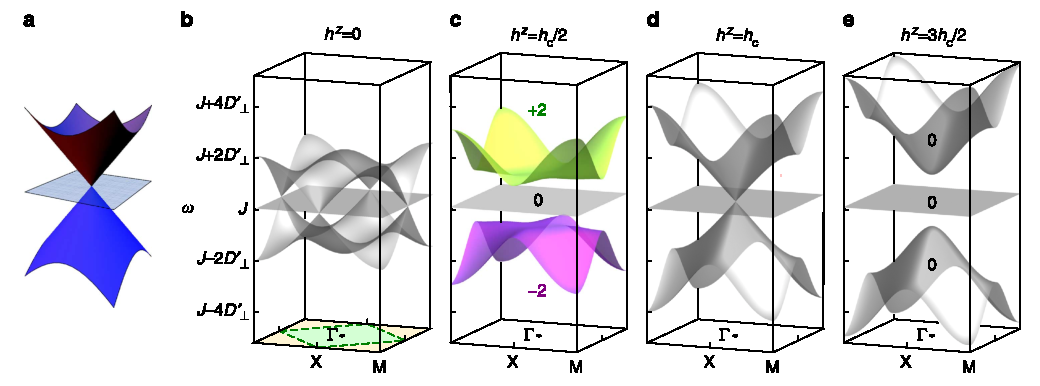
\includegraphics[width=\columnwidth]{figures/SCBO_triplon_bands_Romhanyi.pdf}
	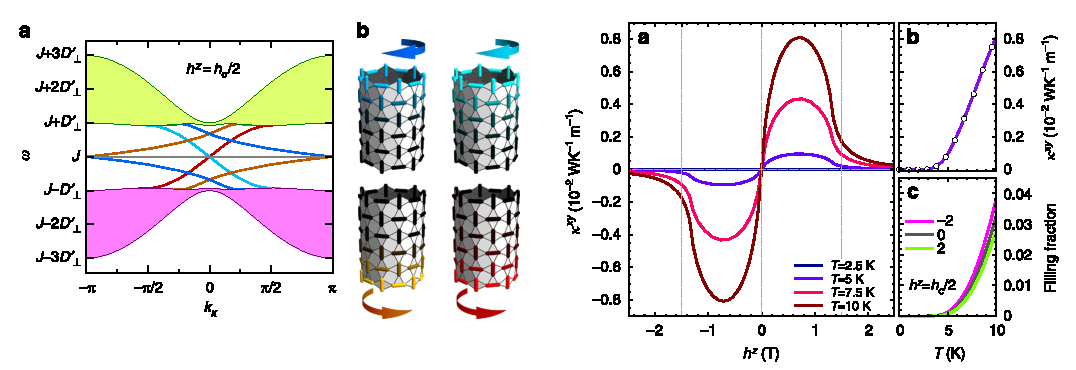
\includegraphics[width=\columnwidth]{figures/SCBO_edge_modes_Romhanyi.pdf}
\end{figure}

With this background in mind, we can now consider what it would mean for the triplon bands in SCBO to have ``nontrivial topology''. Figure \ref{fig:scbo_edge_modes} reproduces several figures from a paper by Romh\'{a}nyi et. al. which computes Chern numbers for the bands generated from the Shastry-Sutherland Hamlitonian, with the DM interaction terms and the applied magnetic field term. What they have shown is that when a magnetic field is applied, a gap opens up between the upper and lower triplon bands, which have Chern numbers of $2$ and $-2$ respectively, and the middle band which has trivial topology (Chern number 0). Then, at a critical field $h_c$, the gaps between the bands close again, opening up above this field to form three bands with trivial topology. As a consequence of the nontrivial topology of the triplon bands, there are 1-D edge states around the edge of the (2-D) Shastry-Sutherland planes. One important feature of these states is that the are chiral: they can only propigate around the edge of the lattice in one direction. Panel f in figure \ref{fig:scbo_edge_modes} shows these states spanning the gap between the bulk triplon bands. The energy of the bands is expressed in terms of the interdimer coupling $J$ and the out of plane component of the interdimer DM interaction $D_\perp$. Each individual band has a group velocity which is either strictly negative or strictly positive. The observation of such an edge state would be compelling evidence for existance of topological triplon bands in SCBO.

\begin{figure}
	\centering
	\caption[SCBO Thermal Hall: Negative Result]{SCBO thermal Hall conductivity at 6K, measured in the Dynacool PPMS. There is no well defined thermal Hall effect observed. Other temperatures measured in the PPMS, as well as our Oxford dilution refridgerator, have borne the same result.}
	\label{fig:scbo_thall_neg}
	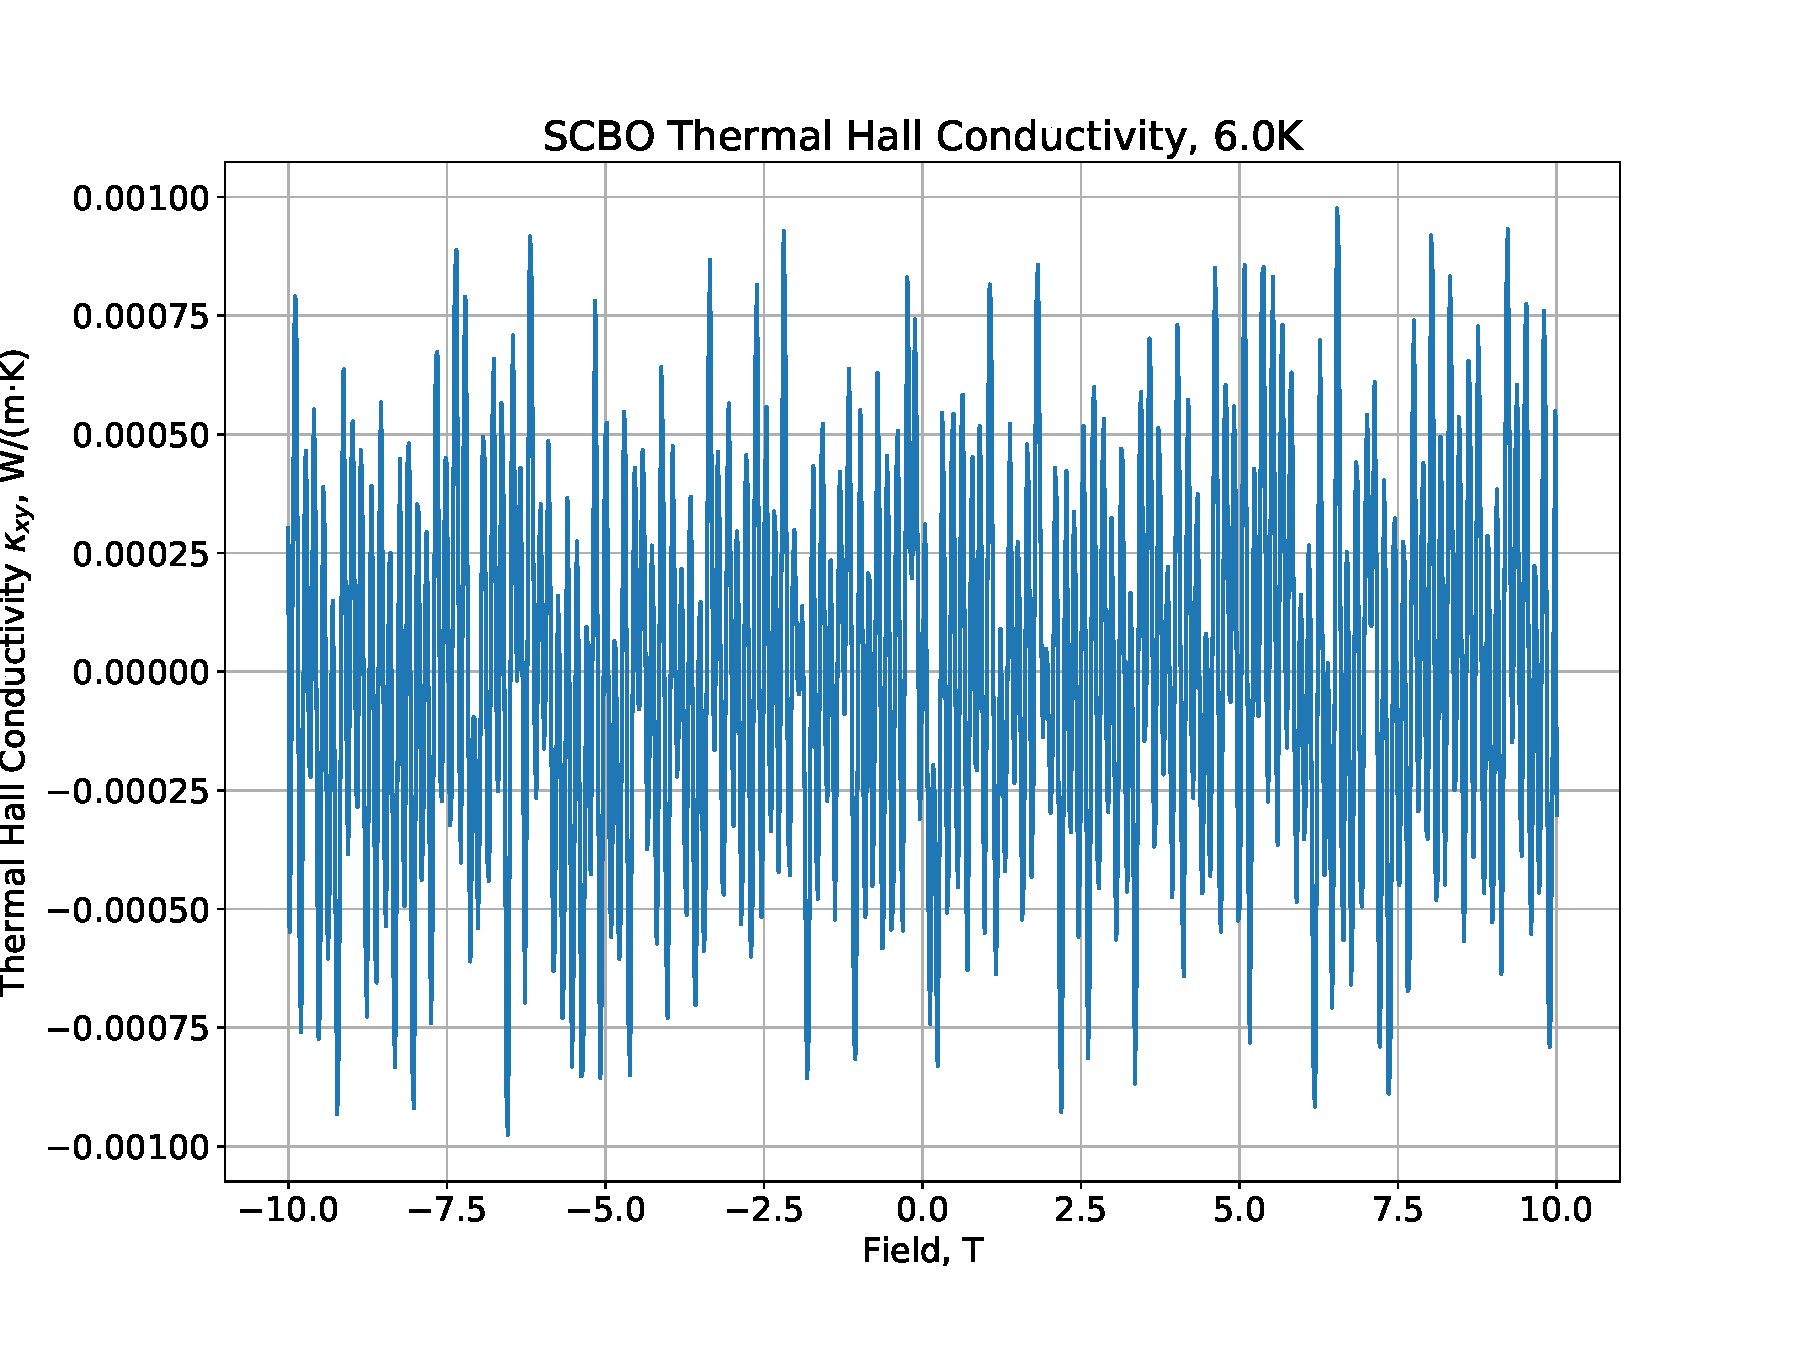
\includegraphics[width=\columnwidth]{figures/SCBO_Thermal_Hall_Negative.pdf}
\end{figure}

The most experiementally relevant prediction made by these calculations, which ties it into the rest of this work, is the presence of a large thermal Hall conductivity. This is ultimately the result of the fact that wave packets in the Chern bands have net rotational motion~\cite{Xiao2010}, with bands of opposite Chern number rotating in opposite directions. For wave packets at the edge of the crystal, this results in unbalanced rotation and a net motion. The triplons with differing Chern numbers have energies which differ by approximately $2D_\perp$, and so those with Chern number $-2$ will be populated preferentially over those with Chern number $2$. It should also be noted that since the triplons are bosons, and so do not form a Fermi pocket, they will need to be thermally activated. Since the triplon bands do not carry any charge, the signature of this motion can only be found using the thermal Hall effect. Panel h of figure \ref{fig:scbo_edge_modes} shows the prediction for the thermal Hall conductivity. As the field is increased, the thermal Hall conductivity is expected to increase to a maximum at half of the critical field $h_c \approx 1.4$ T, then being reduced and heavily suppressed above $h_c$. Panel i of figure \ref{fig:scbo_edge_modes} shows the predicted temperature dependence of the thermal Hall conductivity at $h^z = h_c/2$, increasing dramatically above 5K. The role of the edge states is subtle: they do not contribute directly to the thermal Hall conductivity since edge states of different chirality have the same energy and thus the same occupation, but they do preferentally conduct heat around the edge of the sample, thus populating bulk triplons in the bulk bands near the edge. Regardless, the predicted magnetude of the thermal Hall conductivity is quite large, comparable to that measured in the Bismuth samples discussed in the previous chapter at much higher temperature.

With this in mind, we set out to perform thermal Hall effect measurements on SCBO. Measurements were performed both using the STO capacitave thermometers described in the previous chapter and Cernox resistive thermometers. Both our Oxford dilution refridgerator and the Dynacool PPMS were used as well. After many months of attempts, no signature of the thermal Hall conductivity was found, from temperatures ranging from 0.1 K to 30K and in fields up to 8T. Figure \ref{fig:scbo_thall_neg} shows a representative thermal Hall conductivity trace consisting only of noise, two orders of magnitude below what was predicted by Romh\'{a}nyi et al. Measurements conducted by a group at the University of Edinburgh have corroborated this lack of apparent thermal Hall conductivity~\cite{CairnsMarchMeeting}. This would seem to cast doubt on the existance of topological triplon bands in SCBO. It is difficult to speculate on why this might be the case, but one potential stems from interlayer effects. The calculations in Romh\'{a}nyi et al. assume that the Shastry-Sutherland layers do not interact, but that their individual thermal Hall conductivities add together. However, there is experiemental evidence that there is a coupling $J_{\mathrm{interlayer}}$ between the layers with a magnitude betwen 9\% and 21\% of the interdimer coupling~\cite{Miyahara2000}~\cite{Knetter2000}. These interactions may be frustrated in a similar way to the interdimer coupling, but there could potentially be DM interactions between the planes as well. It is not obvious how these interactions could affect the creation of the Chern bands.

One might get the impression that the months spent trying to resolve the thermal Hall conductivity were a waste. This is far from the truth. As discussed in previous chapters, measurements of the thermal Hall conductivity necissarily require measuring the longitudinal thermal conductivity as well. As it turns out, the thermal Conducitivity of SCBO has a rich structure below 1K. We will discuss these measurements in the next chapter.

\section{Low Temperature Thermal Conductivity in SCBO}

Although our original intention in making thermal measurements was to find the signature of the Chern bands using the thermal Hall effect, the more interesting results come from the thermal conductivity data taken at low temperatures. The data was originally taken at constant temperature as a function of applied magnetic field. Two datasets were collected: One from 6 K down to 2 K every 1 K taken using the Dynacool PPMS, and one from 1 K to 100 mK at least every 100 mK with denser curves at some particular temperature ranges, taken in our Oxford Dilution refridgerator. The sample used in the PPMS was approximately rectangular with total dimensions of 2.5 mm long by 0.85 mm wide by 0.2 mm thick. The longitudinal distance between the thermometers in the PPMS measurements was 0.75 mm. For the dilution refridgerator experiments, the sample was 3.1 mm long by 1.3 mm wide by 0.2 mm thick, with a longitudinal distance between the thermometers of 0.78 mm. The relatively small longitudinal distances were chosen since we were still trying to detect a thermal Hall signal as well as measure the thermal conductivity. The samples were oriented so that the magnetic field was applied along the c axis, i.e. perpendicular to the Shastry-Sutherland planes.

Earlier thermal conductivty measurements attempted to use STO capacitive thermometers, but since the interesting signal occurs primarily below 4 K, the unannealed thermometers were not suitable. Thus, a matched pair of bare chip Cernox thermometers was used instead. The detailed magnetoresistance of these thermometers was mapped in situ and all temperatures derived from this field calibration. For the PPMS data, a sine wave excitation of 0.1 mA and a period of 200 s was applied to the resistive heater. The relatively large excitation was once again used to give the best chance of finding a thermal Hall signal. For the dilution fridge data, the same period was used, but the excitation used ranged from 58.57 $\mu$A at 1 K to 10 $\mu$A at 100 mK. The large range in excitations was necessary since the temperatures involved spanned an order of magnetude. Excitations were selected to ensure that the temperature difference between the thermometers was less than either 1\% of the total temperature, or 10 mK if that did not provide enough sensitivity.


\begin{figure}
	\centering
	\caption[Low Temperature Thermal Conductivity of SCBO]{Low Temperature thermal conductivity of Strontium Copper Borate. Each curve is taken at a constant temperature. Top: Data taken in the Dynacool PPMS, from 6 K to 2 K. The applied field enhances the thermal conductivity. Bottom: Data taken in the Oxford dilution refidgerator, from 1 K down to 100 mK. Field supresses the thermal conductivity down to about 450 mK, at which point the dependence flips around again.}
	\label{fig:SCBO_kappa_xx}
	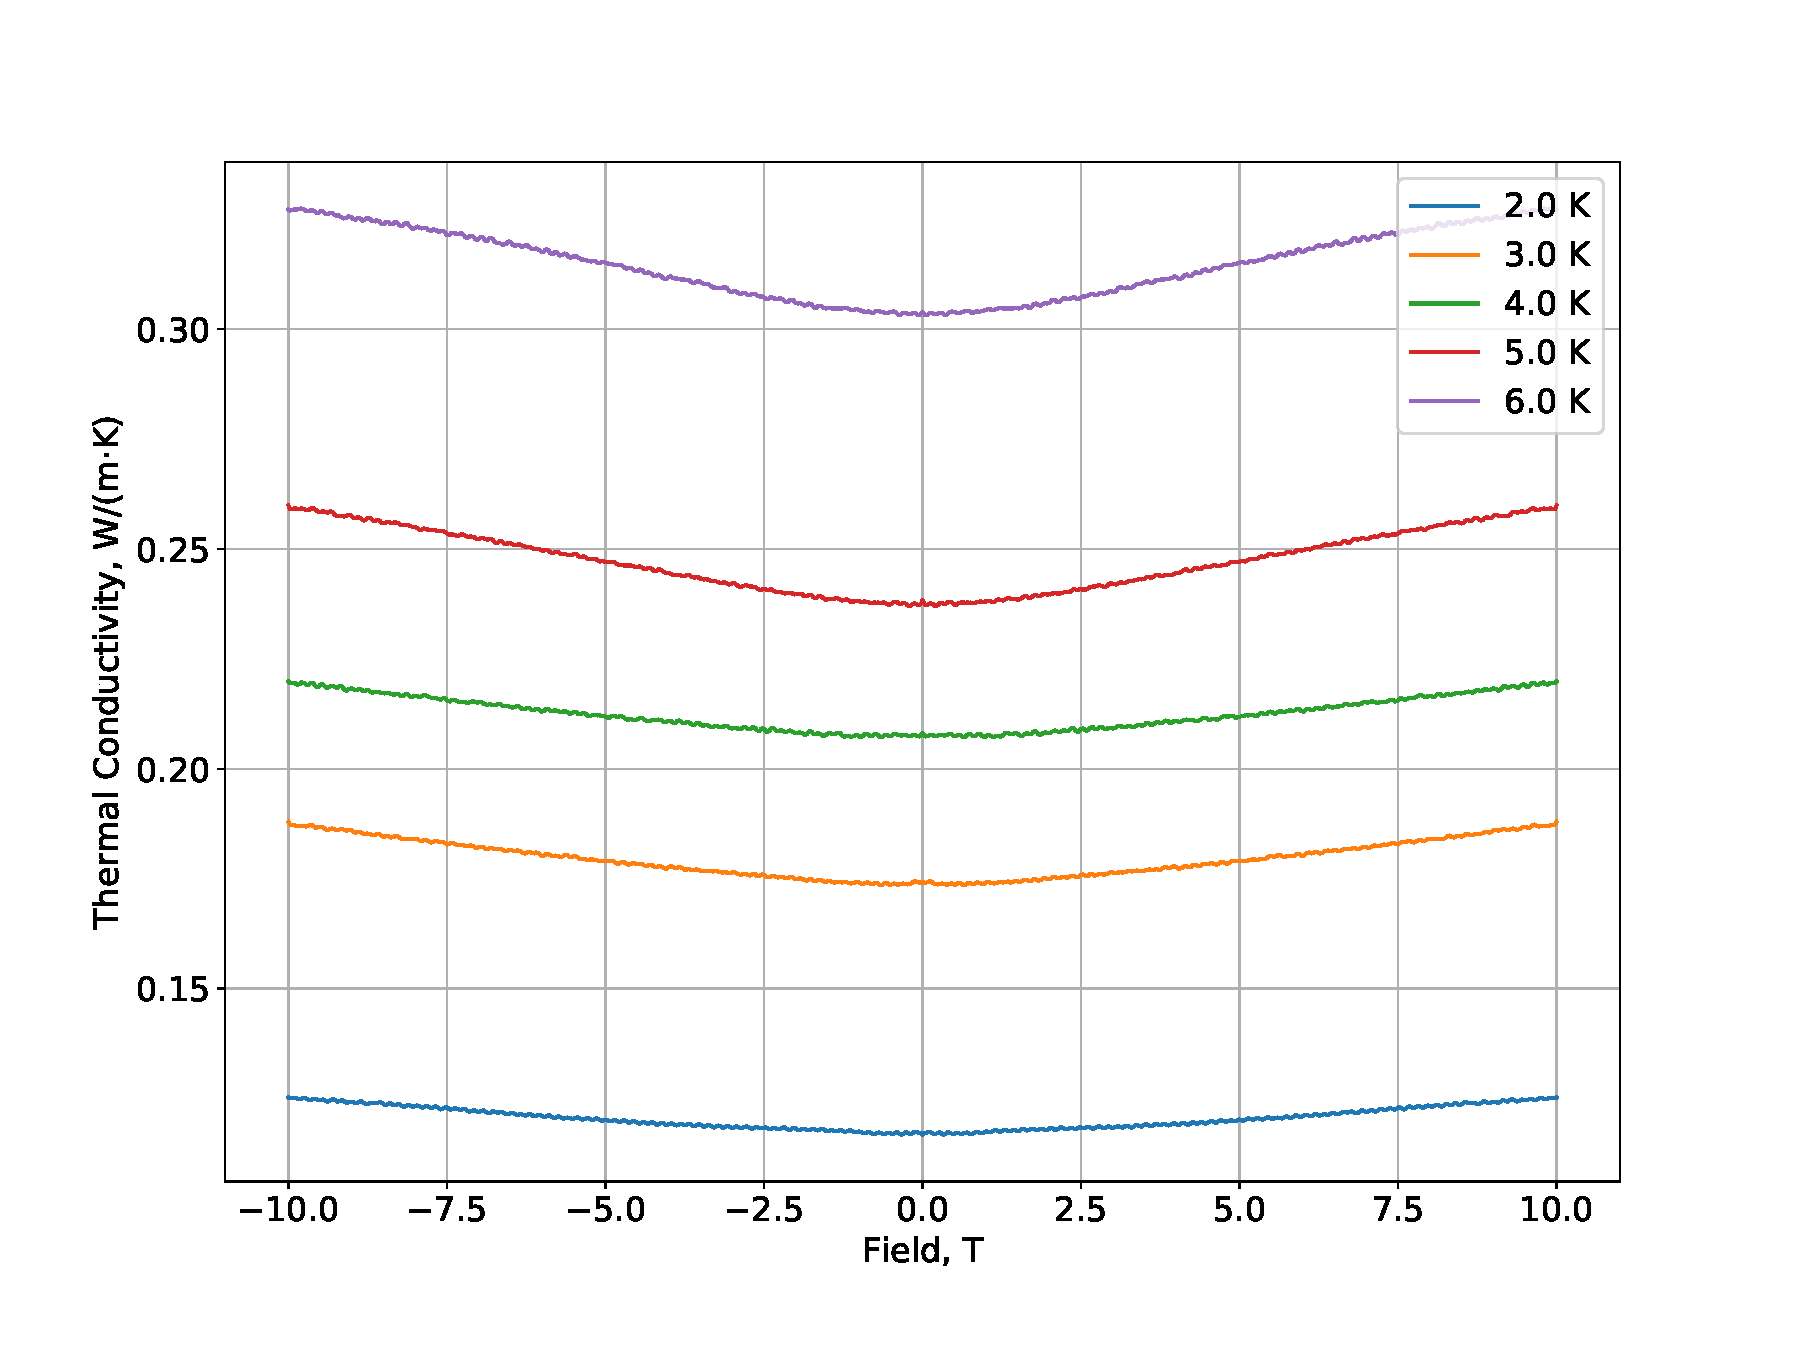
\includegraphics[width=0.9\columnwidth,trim={1cm 1cm 1cm 1cm},clip]{figures/SCBO_tcond_high.pdf}
	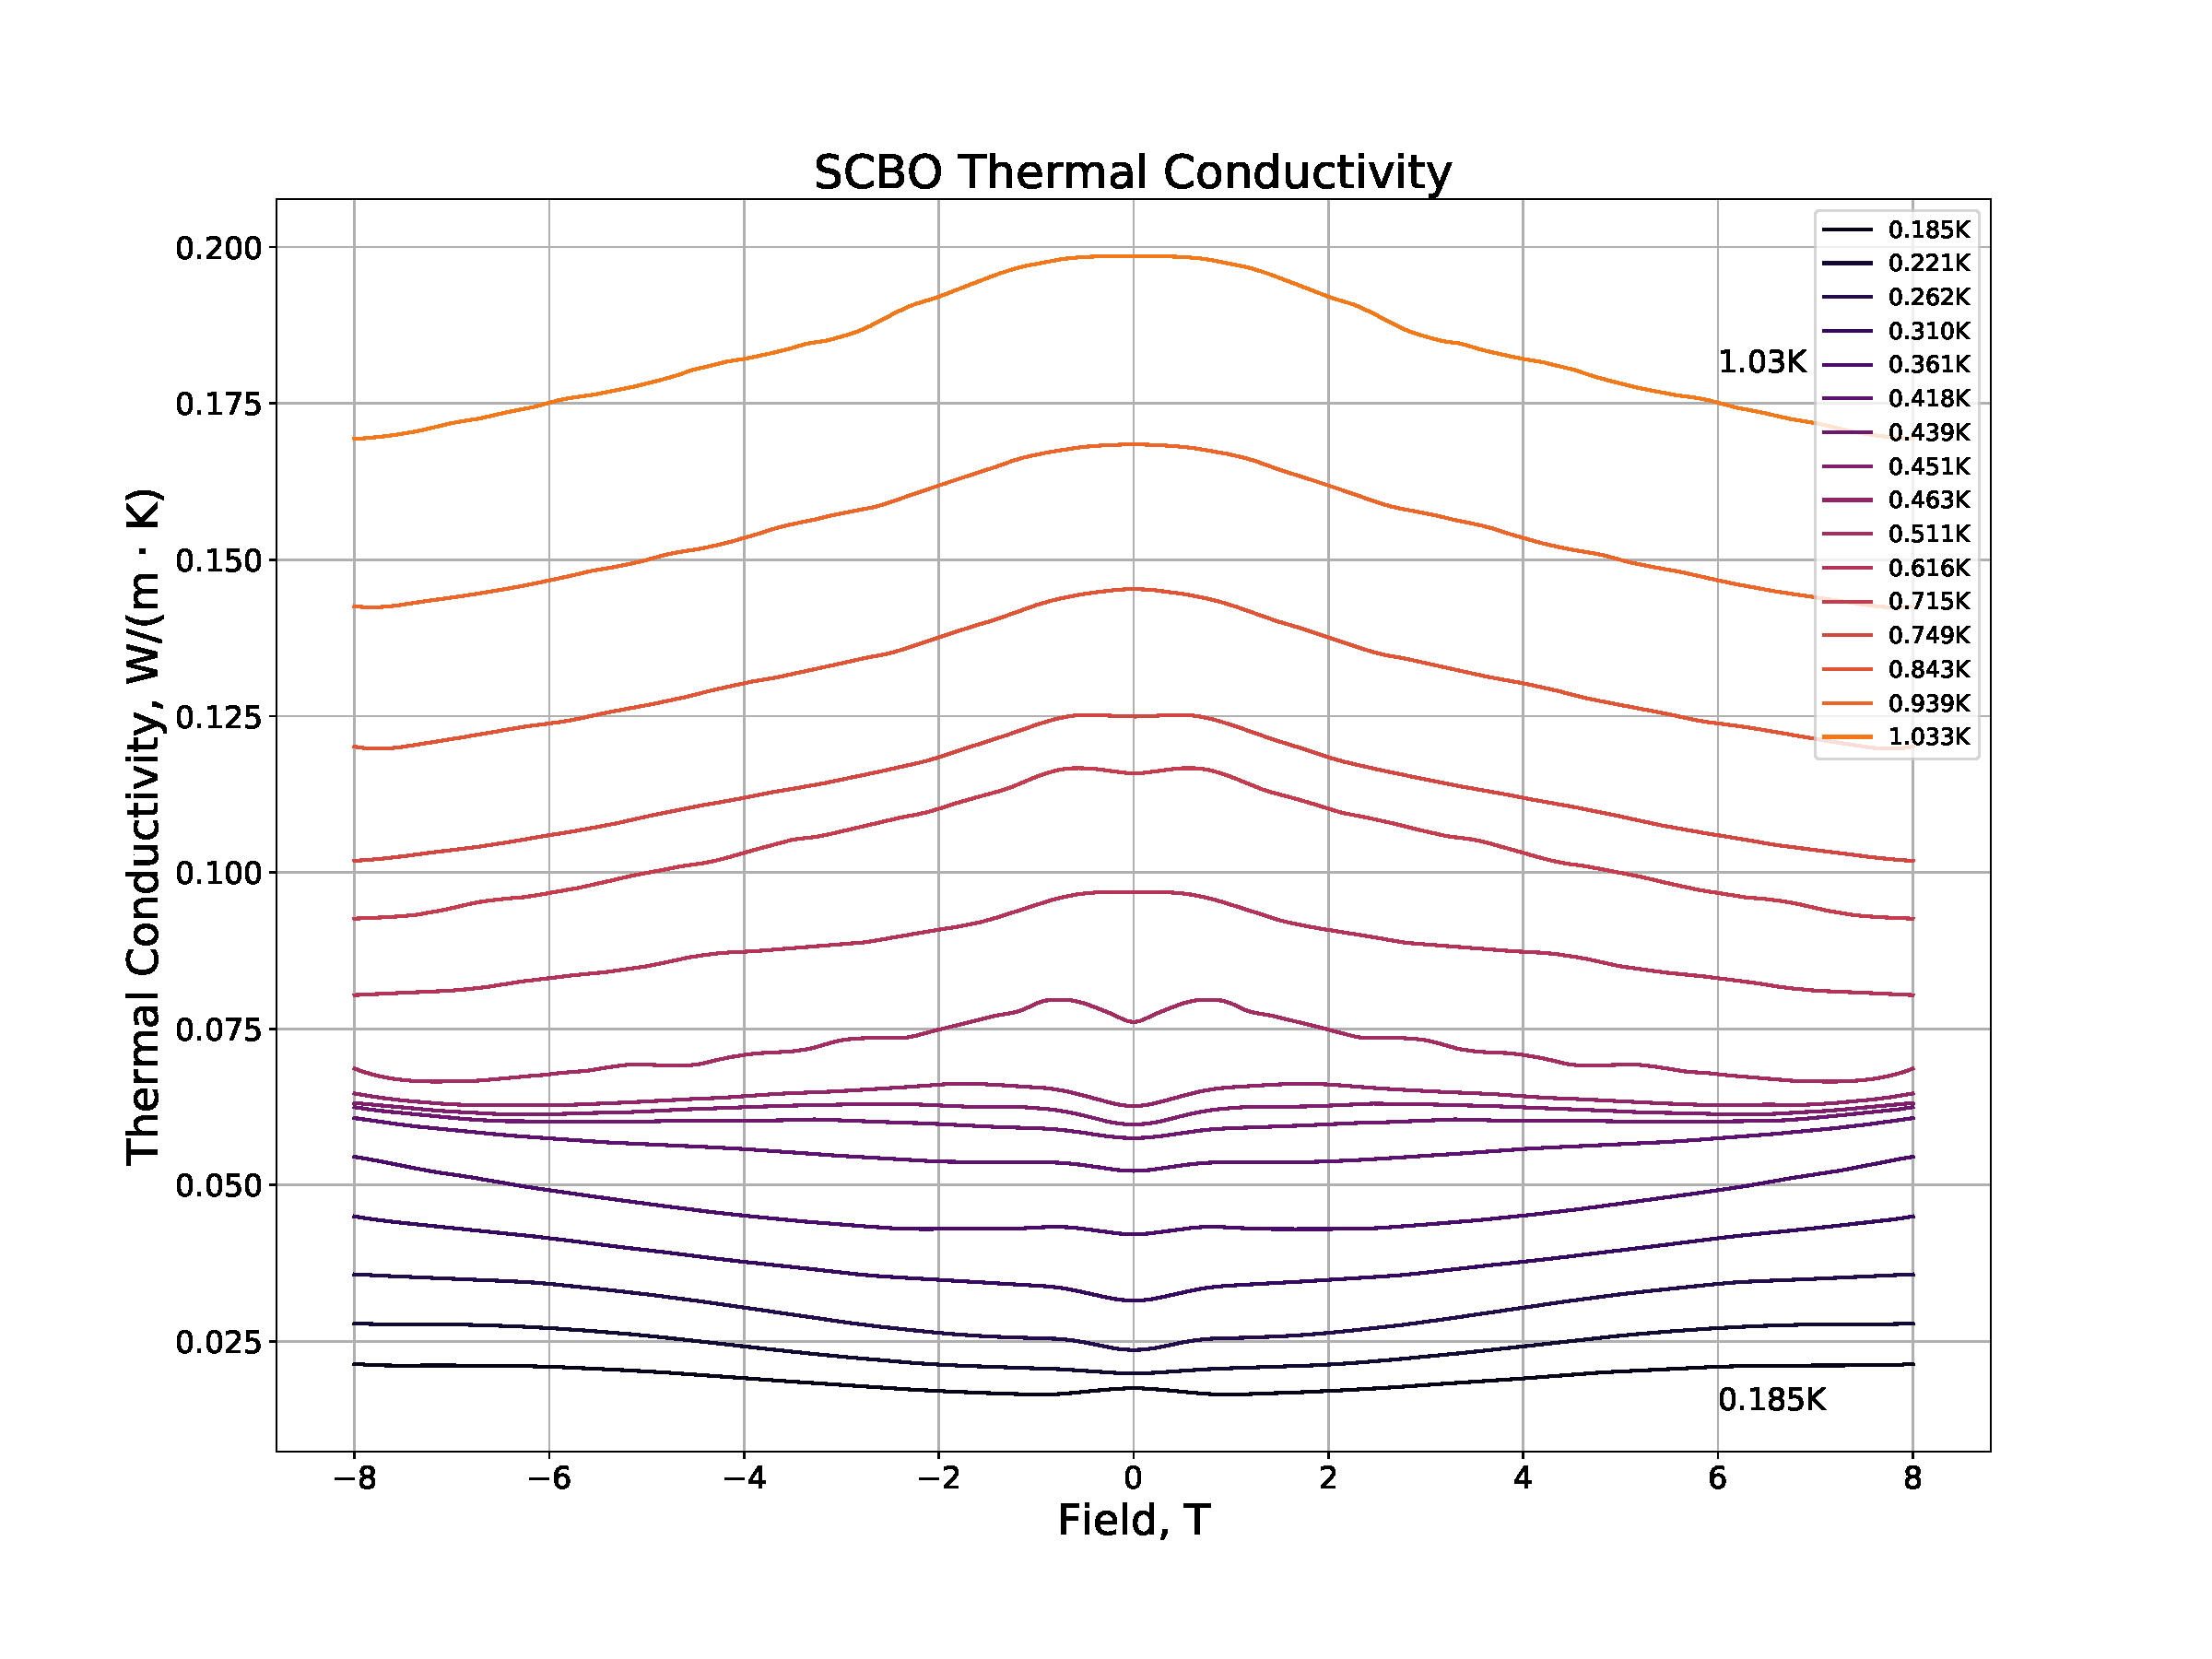
\includegraphics[width=0.9\columnwidth,trim={1cm 1cm 1cm 1cm},clip]{figures/SCBO_kappa_xx_vs_B_1.pdf}
\end{figure}

The thermal conductivity data found in these experiements is summarized in figure \ref{fig:SCBO_kappa_xx}. The top panel shows the data taken in the PPMS. In this data, the application of the magnetic field appears to enhance the thermal conductivity, with the effect weakening as we cool down to 2 K. The bottom panel shows the data taken in the dilution fridge. Here, it appears that the magnetic field supresses the thermal conductivity at 1K, but when the temperature is lowered to around 450 mK, the dependence begins to flip around. At lower temperatures, the thermal conductivity is instead enhanced by magnetic field. The same dataset is plotted in figure \ref{fig:SCBO_kappa_xx_vs_T}, this time with cuts taken at constant magnetic field as a function of temperature. Seperate data runs where the temperature was ramped at a constant magnetic field were taken which reproduce the general trends of this data, however they suffer from a great deal of noise due to the massively different excitations required at each temperature. Figure \ref{fig:SCBO_kappa_xx_vs_T} makes the ``crossover'' between magnetic field supression and enhancement of the thermal conductivity at around 450 mK more clear. This crossover is not sharp in the sense that the conductivity traces do not converge to a point. This would correspond to the thermal conductivity being independent of magnetic field at some temperature, instead we see that some traces show enhancement and supression at different values of the applied field. Not included in this plot is the data taken in the PPMS. In that dataset, we can see that the value of the thermal conductivity taken at 2K is lower than that taken at 1K in the dilution fridge. It is unclear if this is a true effect or if it is an error introduced by uncertianty in the sample geometry. Previous measurments of the thermal conductivity at higher temperatures have shown that the temperature dependence at higher temperatures is indeed not monotonic~\cite{Hofmann2001}, but it is difficult to do an experiement in our systems which would show this conclusively. The PPMS cannot stabilized temperature lower than 2 K due to the custom puck required to do the measurement, and the dilution fridge cannot control temperature in the range between 1 K and 2 K due to competition between the dilution unit and the pulse tube stage. Thus, for the remainder of this section we will focus on the dilution fridge data, which shows a clear inversion of the field dependence.

\begin{figure}
	\caption[Temperature Dependence of SCBO Thermal Conductivity]{The same data set as \ref{fig:SCBO_kappa_xx}, now plotted with temperature on the x axis instead of magnetic field. Each trace is a particular cut through the data at a constant field. The crossover between supression and enhancment of the thermal conductivity is evident at around 450 mK.}
	\label{fig:SCBO_kappa_xx_vs_T}
	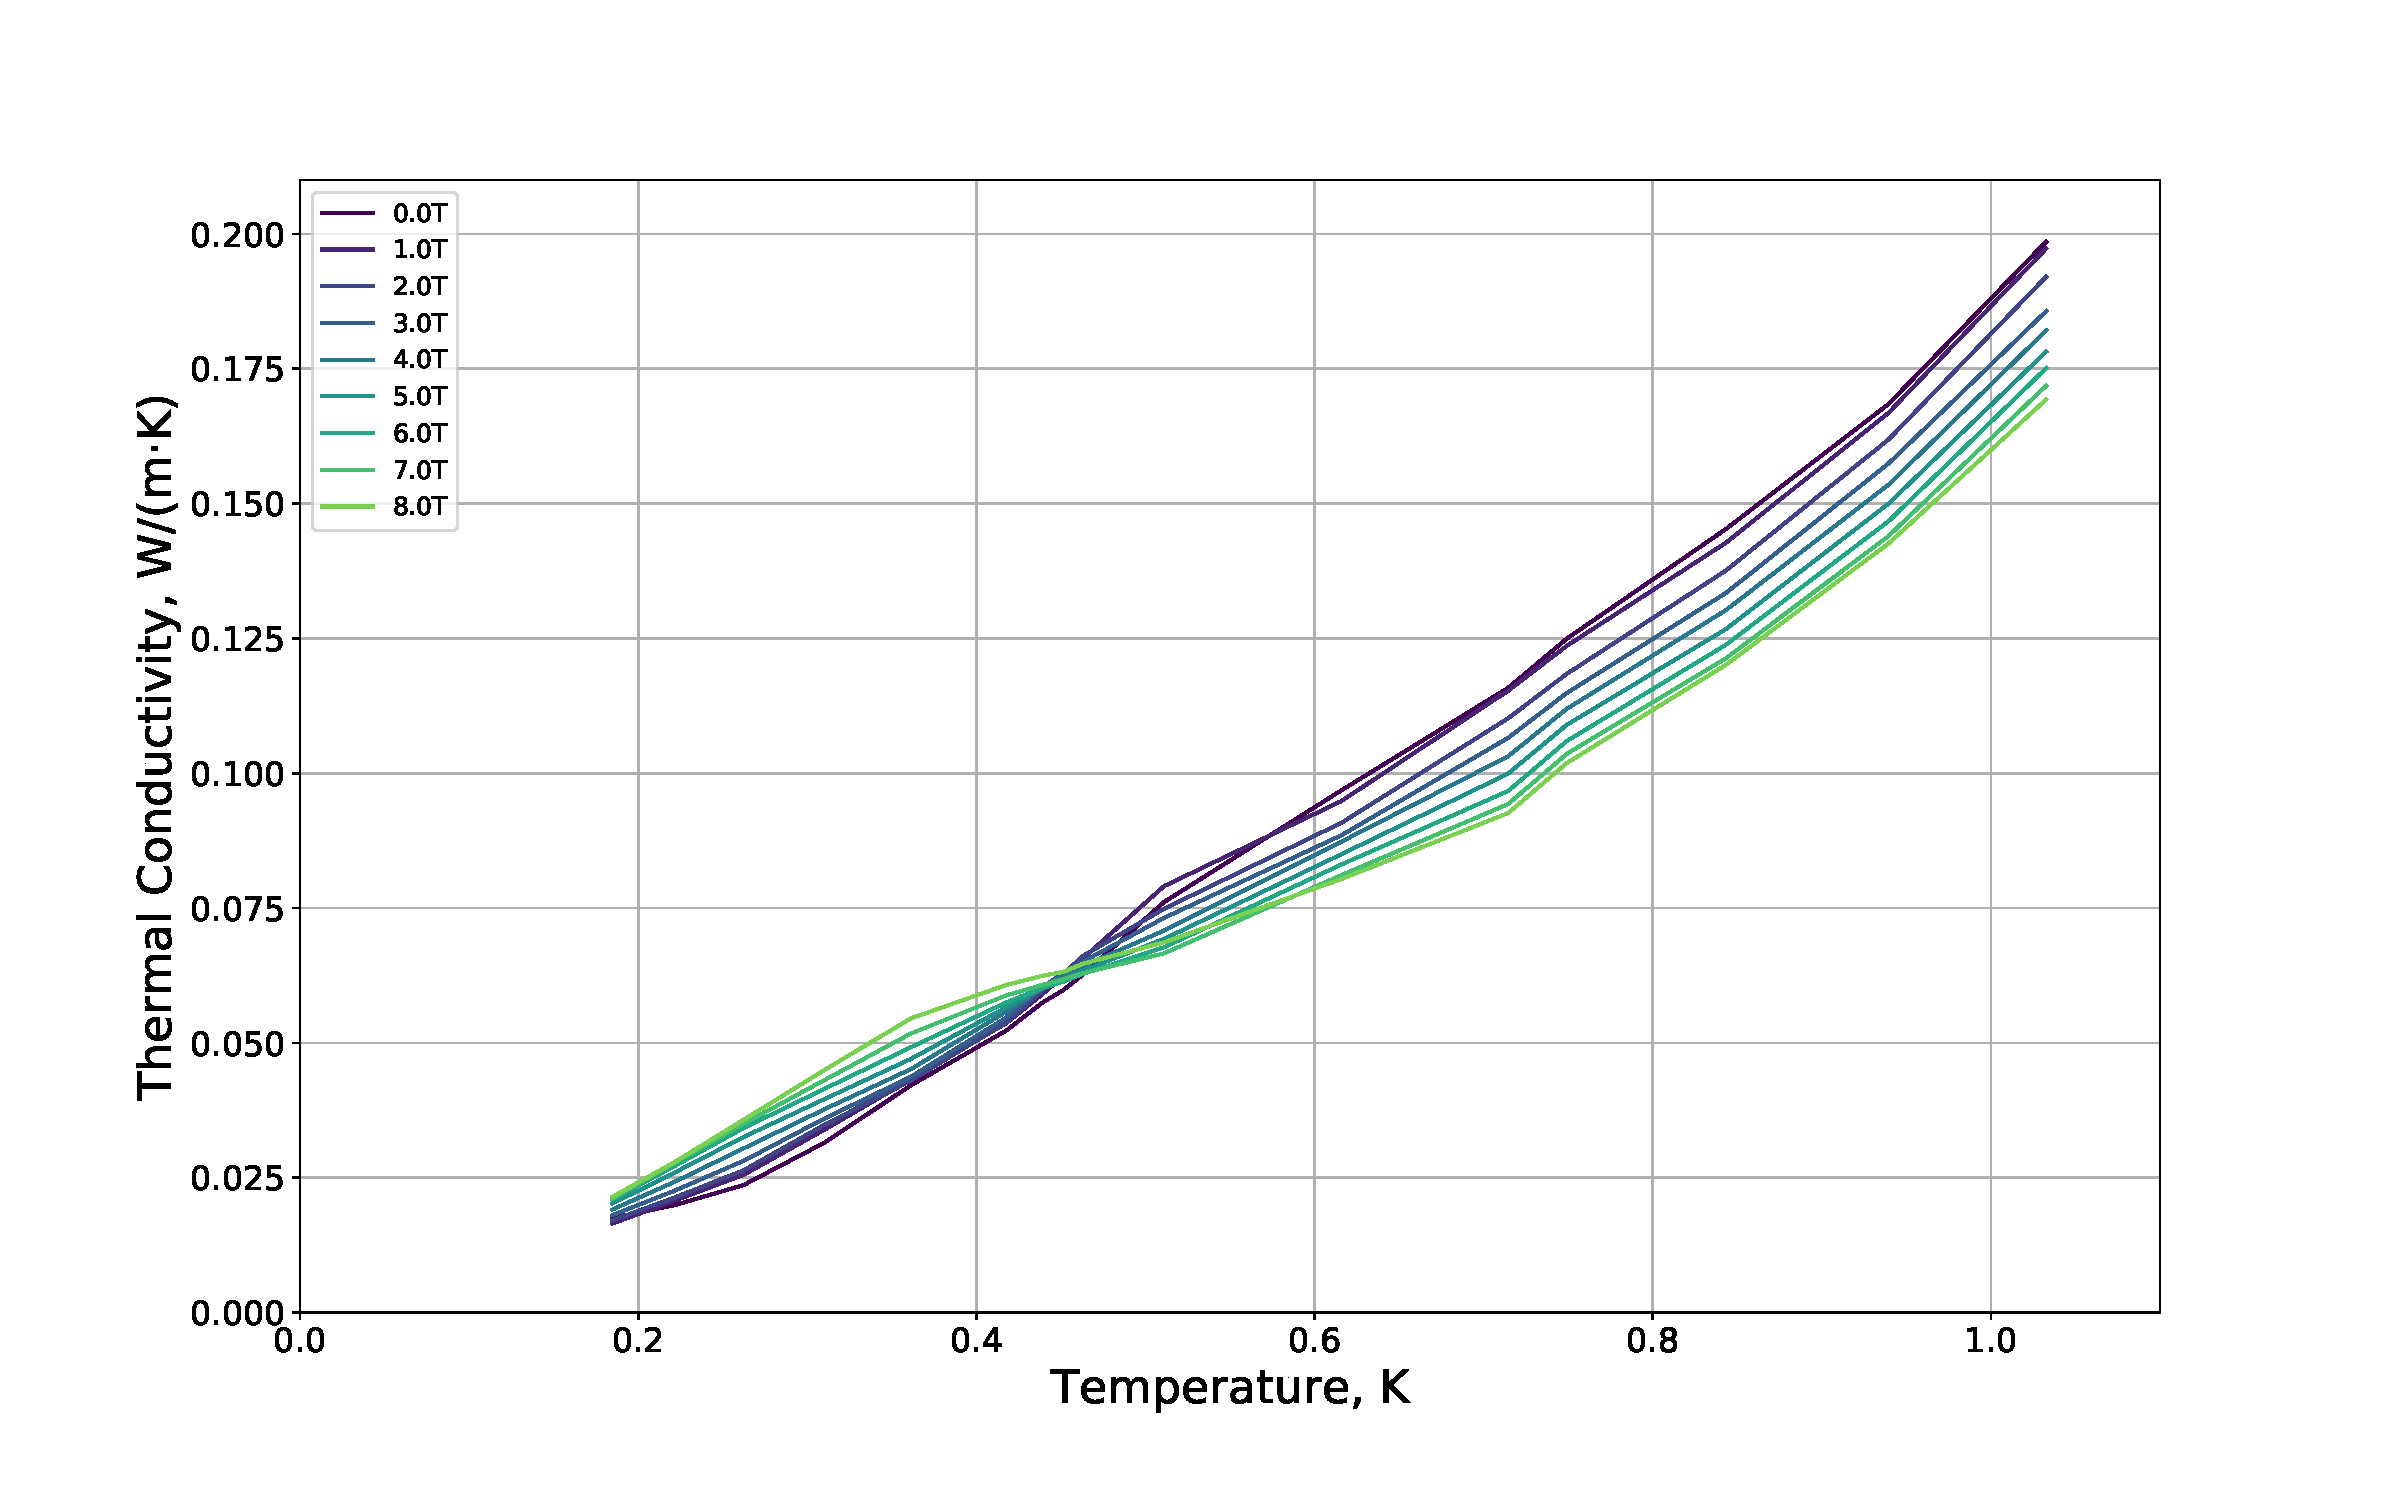
\includegraphics[width=\columnwidth]{figures/SCBO_kappa_vs_T.pdf}
\end{figure}

The presence of a field dependant thermal conductivity in this temperature range is very puzzling. Certianly we can imagine that the triplons should couple to a magnetic field, but since the gap between the triplons and the singlet ground state has been observed to be about 3 meV (see figure \ref{fig:scbo_triplon_bands}), corresponding to about 35K, we should expect that the occupation of triplons should be extremly small. In any event, since the triplons have very flat dispersion, they should not contribute much to the thermal conductivity even when they are occupied. The phonons themselves should also not couple to a magnetic field directly. However, it has been noted in previous measurements of the thermal conductivity at higher temperature~\cite{Hofmann2001} as well as the heat capacity~\cite{Jorge2005} were significantly influcence by resonant scattering of the phonons by the triplon states. This resonant scattering is observed to significantly supress the thermal conductivity by damping the phonons. As discussed above, this resonant scattering is also responsible for an anomaly in the thermal conductivity around 7.5 K. This mechanism could certianly couple the thermal conductivity to the magnetic field, but it appears to do so in the wrong temperature range. The effect of this anomaly is already small at 2.5 K, but the thermal conductivity is still being affected by the field down to 200 mK. In that section we also noted that the DM interaction could mix the singlet and triplet states since it violated conservation of $s^z$. The signature of resonant scattering by these states was present in the heat capacity measurement at lower temperatures, but only in fields above 10 T. In the thermal conductivity measurement, it appears the bulk of the change in $\kappa_{xx}$ occurs below 5 T. Heat capacity measurements at lower temperatures would certianly help to disambiguate this phenomena, but from the data presented it seems like the field scale is wrong for this to be a factor.

\begin{figure}
	\caption[Example fits of SCBO data.]{Example fits of the Strontium Copper Borate thermal conductivity data. Above and below the crossover region, the ansatz fits quite well. In the crossover region, however, the thermal conductivity appears to have more structure than what is captured by the ansatz.}
	\label{fig:SCBO_example_fits}
	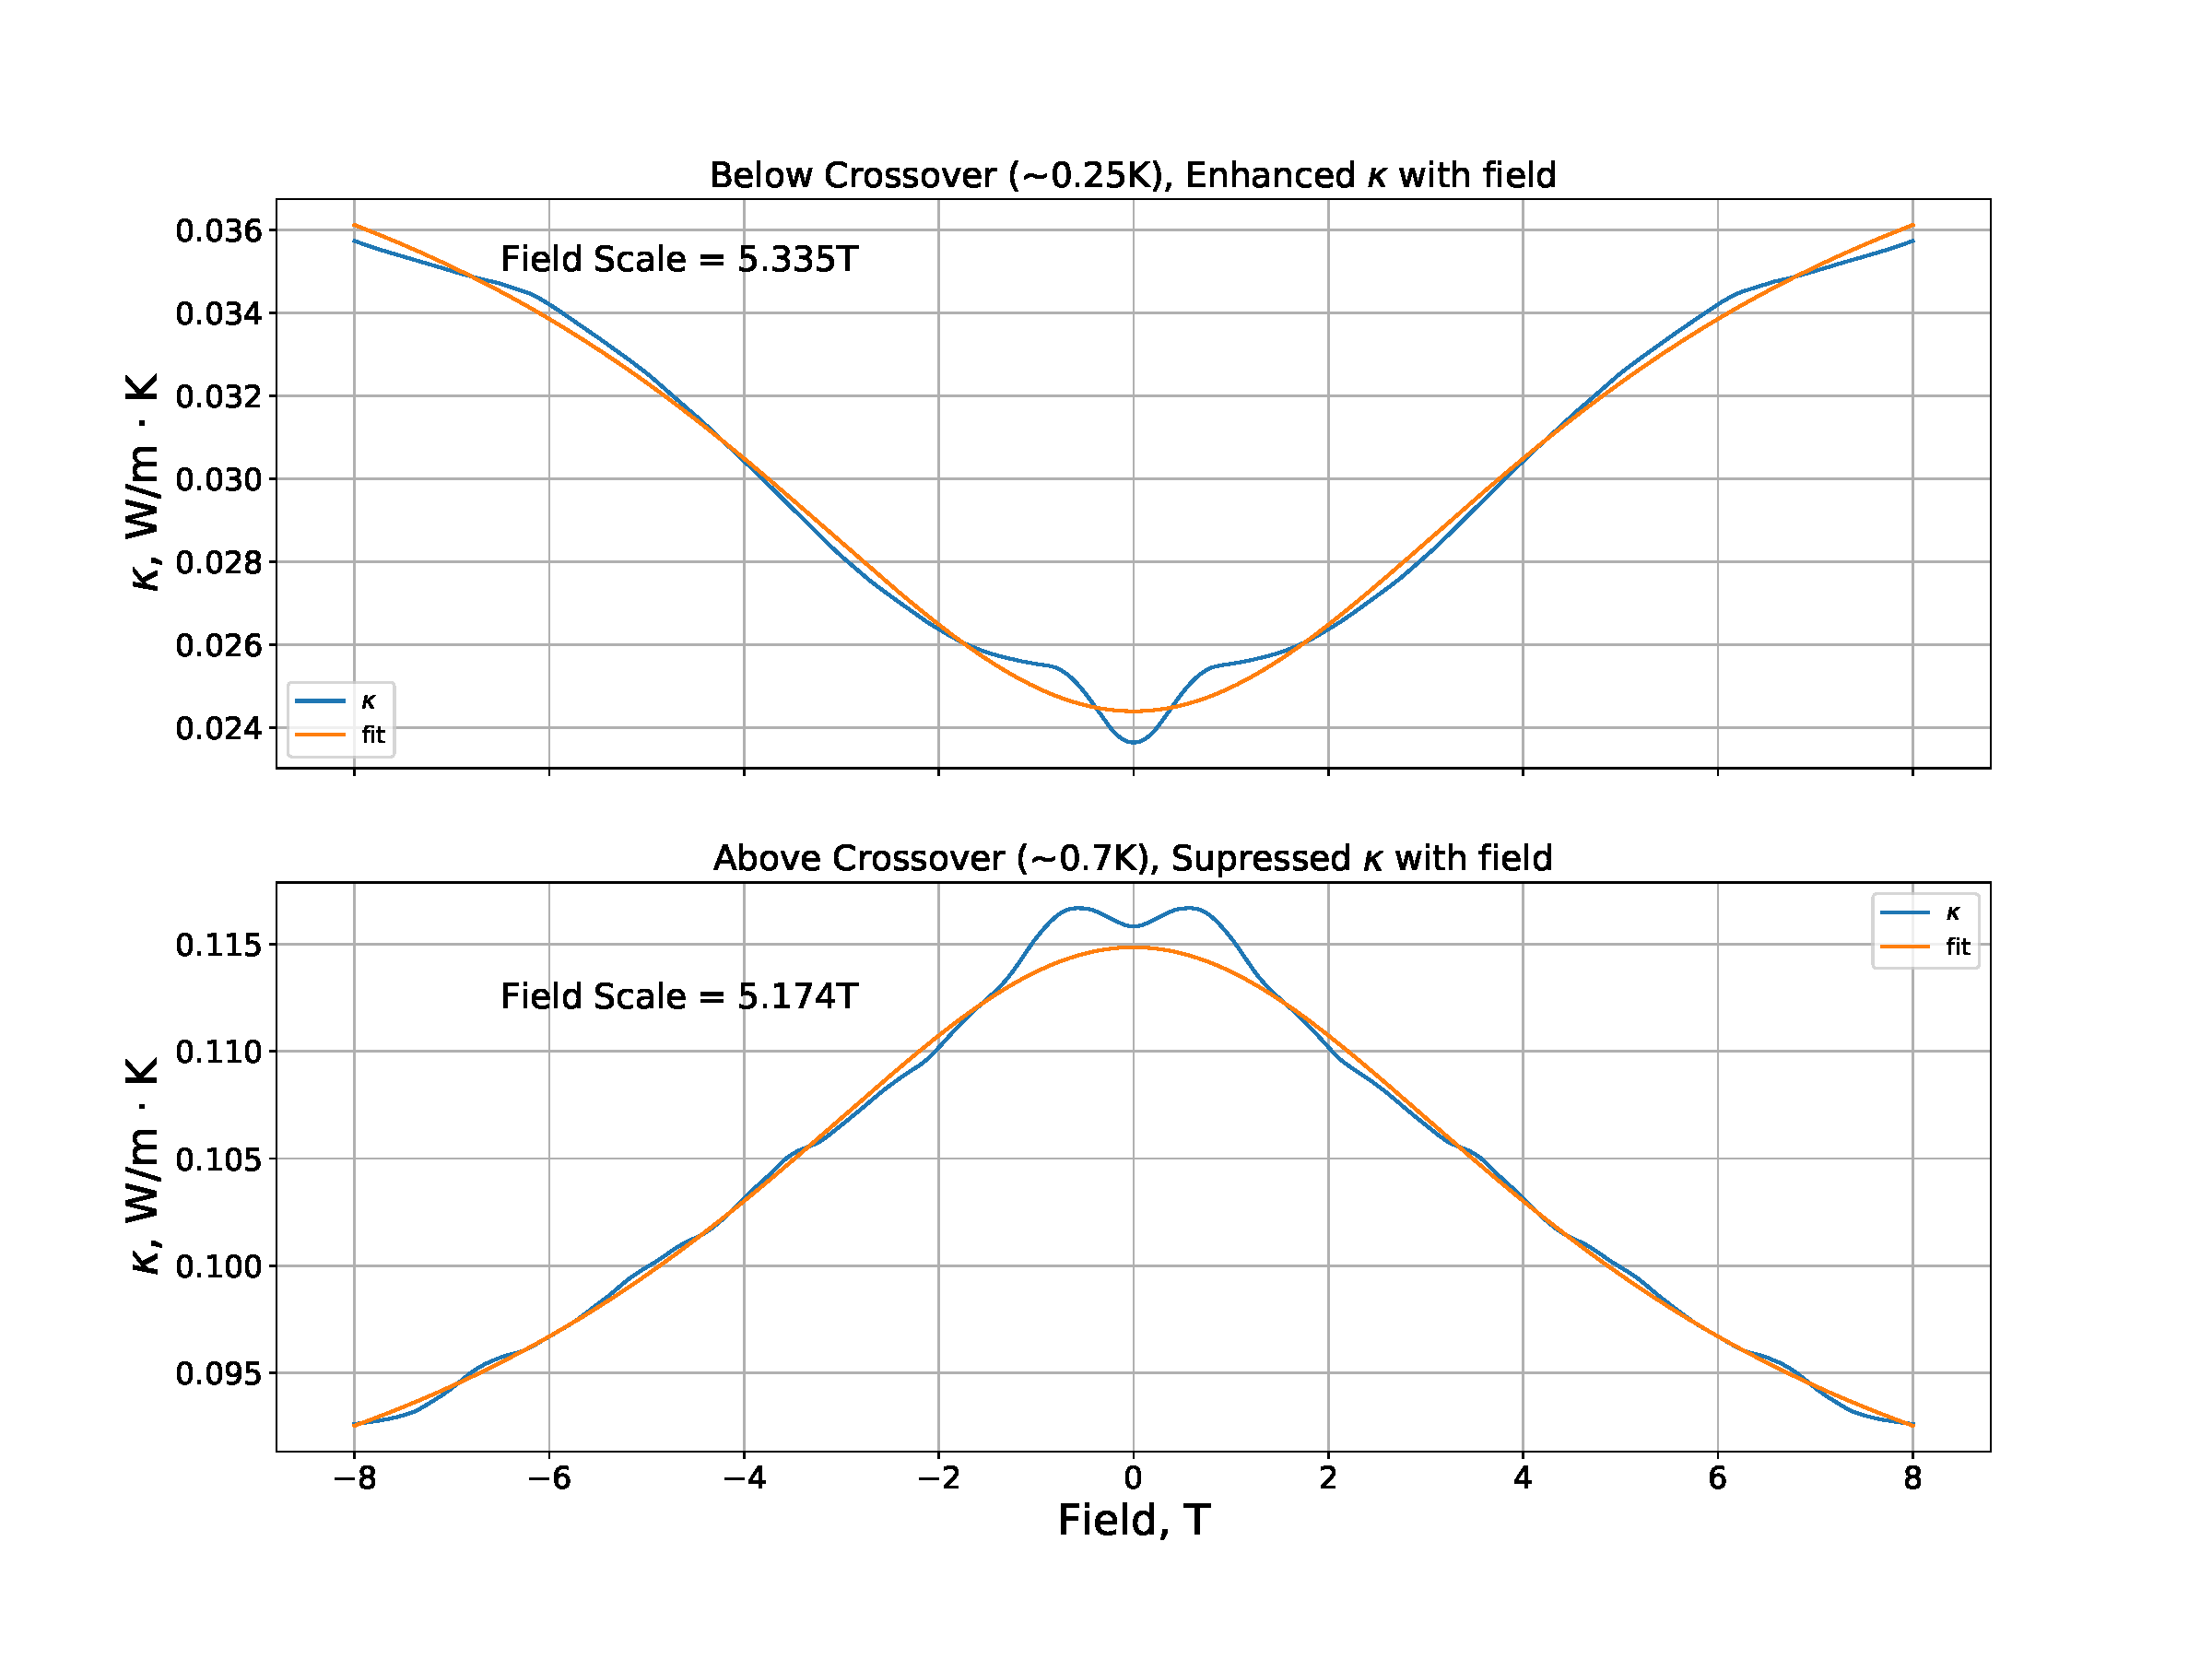
\includegraphics[width=\columnwidth]{figures/SCBO_kappa_vs_b_fits.pdf}
\end{figure}

Although we no not have a good theoretical explaination for the changing thermal conductivity in this tempereature range, we still wish to find some way to quantify the changes. Qualitiatively, most of the curves appear to start at some value and then asymtotically move towards some other value at high fields, lower in some cases and higher in others. In order to structure our thinking, we have fit these curves to a function which has this qualitative structure:
\[ \kappa_{xx}(h) = a + \frac{c}{1 + (h/b)^2}\]
where $h$ is the applied field, and $a$, $b$, and $c$ are the fit parameters. These parameters have straightforward interpretations: $a$ is the infinite field thermal conductivity, $c$ is the difference between the zero field and infinite field conductivities (so that $\kappa_{xx}(0) = a + c$), and $b$ is a ``field scale'' which characterizes the width of the transistion between the zero and infinite field values. Thus, when the field is multiple times higher than this field scale, we expect the thermal conductivity to be more or less constant. Figure \ref{fig:SCBO_example_fits} shows a few example fits. For traces taken above and below the crossover region, the fit appears to work quite well, independent of the sign of $c$. For the traces in the transistion region, however, the fits do not capture all of the structure of the thermal conductivity. The derivative of $\kappa_xx$ with respect to the field appears to oscillate a few times, and it is unclear if it has an infinte field asymtote. A summary of the fitted parameters is shown in figure \ref{fig:SCBO_fit_params}. Both plots have error bars extracted from the fits plotted in red. For the traces in the crossover region, where the fit is not adequite, the error bars are quite large. However, above and below it, they are relatively small. The top panel shows the extracted field scale. For all the plots outside the crossover, the field scale is more or less independent of temperature, with an average of 5.19 T. Since we are able to apply fields of up to 8 T in the Oxford dilution fridge, we can be confident we have enough field to capture this feature. The bottom panels shows the zero field ($a + c$) as well as the infinite field ($a$) thermal conductivity. 

Very recently, a similar crossover effect has been observed in a layered magnet CrCl$_3$, studied for its similarity to the spin liquid candidate $\alpha$-RuCl$_3$~\cite{Pocs2019}. In that material, the crossover from enhancment to supression of the thermal conductivity in field is explained by a transition from coherent conduction by magnons to scattering of phonons by magnons being the dominant factor affecting the thermal conductivity. While there is good reason to suspect resonant scattering by triplons is playing an important role at higher temperatures in SCBO, the fact that the magentoconductivity persists down to 200 mK presents a problem for applying this explaination in SCBO. As far as scattering by the triplons are concerned, they provide a schematic model for thermal conductivty in a system with phonons scattered by magnons:
\[\kappa^{-1}(H,T) = \kappa^{-1}_{\mathrm{ph}}(T)[1 + \lambda(H,T)n_{\mathrm{mag}}(H,T)]\]
where $\kappa$ is the total thermal conductivity, $\kappa_{\mathrm{ph}}$ is the field independent phonon component, $n_{\mathrm{mag}}$ is the population of magnons, and $\lambda$ characterizes the strengh of the coupling. the quantity $\lambda n_{\mathrm{mag}}$ is effectively ratio between the scattering rates of phonons between the lattice and the magnons. However, at 500 mK, based on Bose-Einstien statistics, the occupation of triplons should be less than one in ten thousand \textit{per mole of dimers}! In order to for resonant scattering to explain the thermal magnetoconductivity in this range, we would need $\lambda$ to be so large as to be completely unphysical. 

\begin{figure}
	\centering
	\caption[SCBO Fitting Parameters vs. Temperature]{Top: Extracted field scale vs. temperature. The red lines are the error bars from the fit. Note that the field scale is more or less constant where the fit is valid. Where it is not valid, the error bars extend beyond the scale of the plot. I have kept them here to demarkate the crossover region. Bottom: Zero field (blue) and infinite field (green) thermal conductivities extracted from the fits. Once again the error bars are red.}
	\label{fig:SCBO_fit_params}
	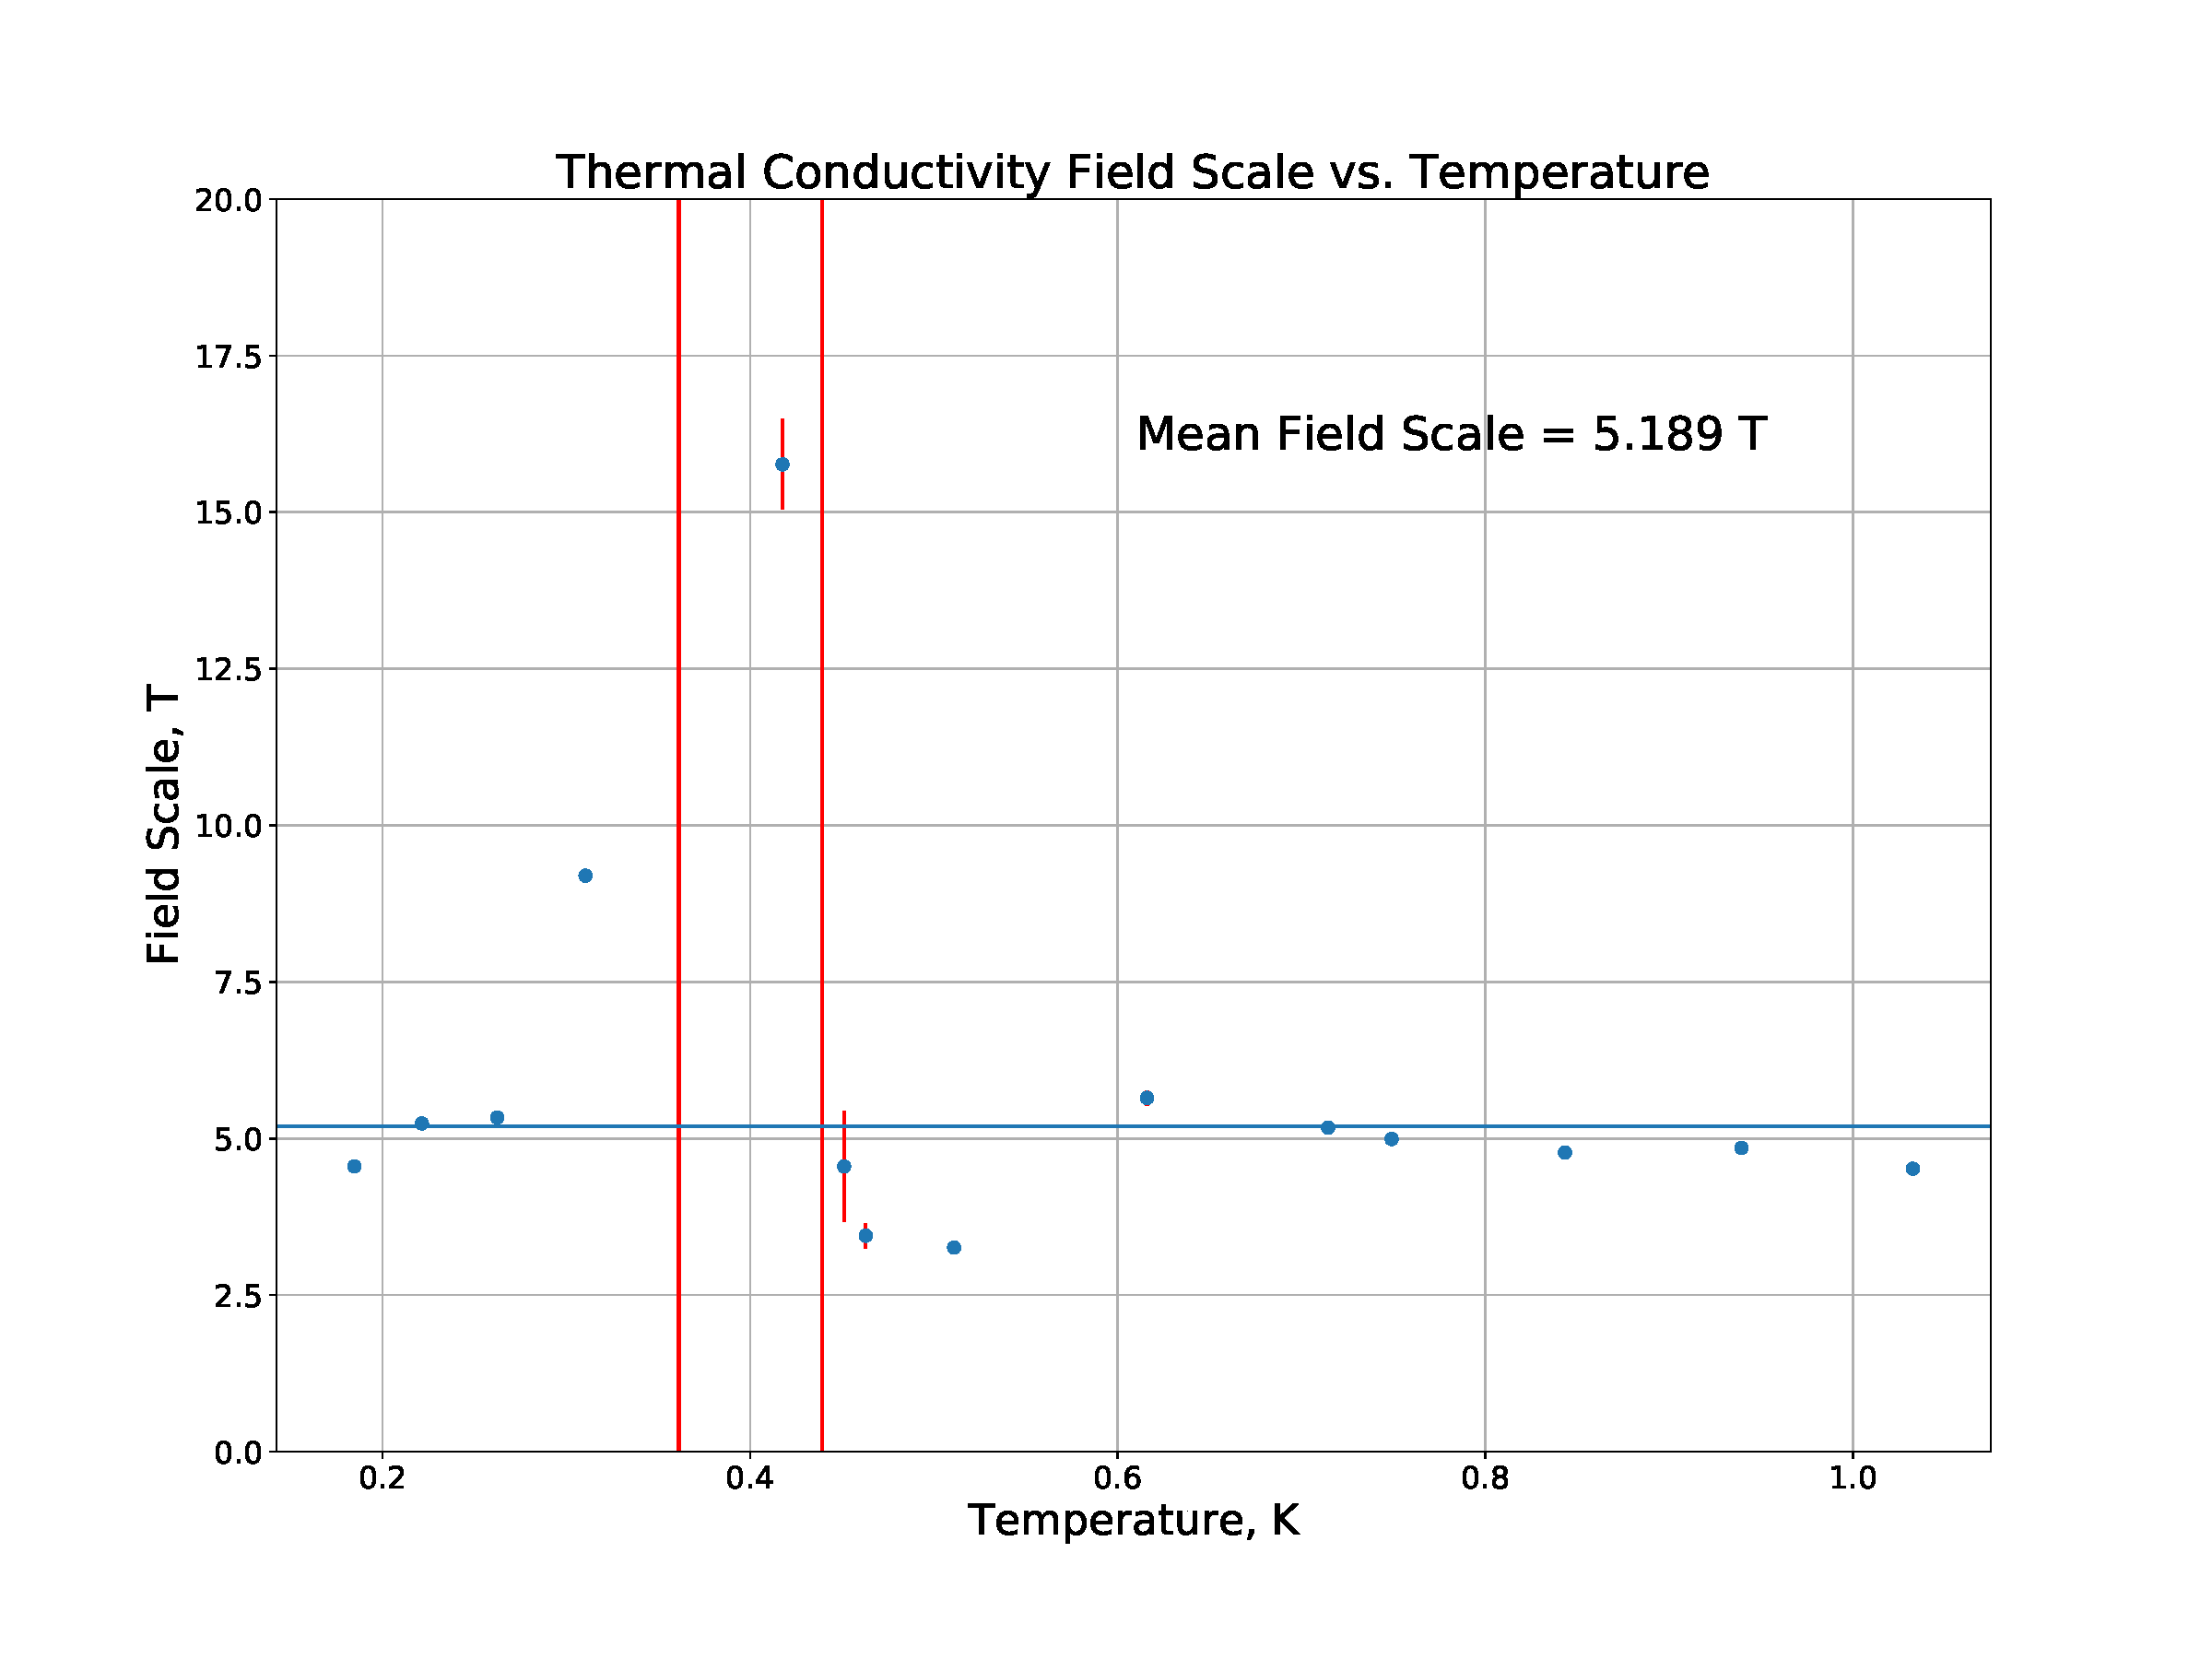
\includegraphics[width=0.9\columnwidth,trim={1cm 1cm 1cm 1cm},clip]{figures/SCBO_field_scale.pdf}
	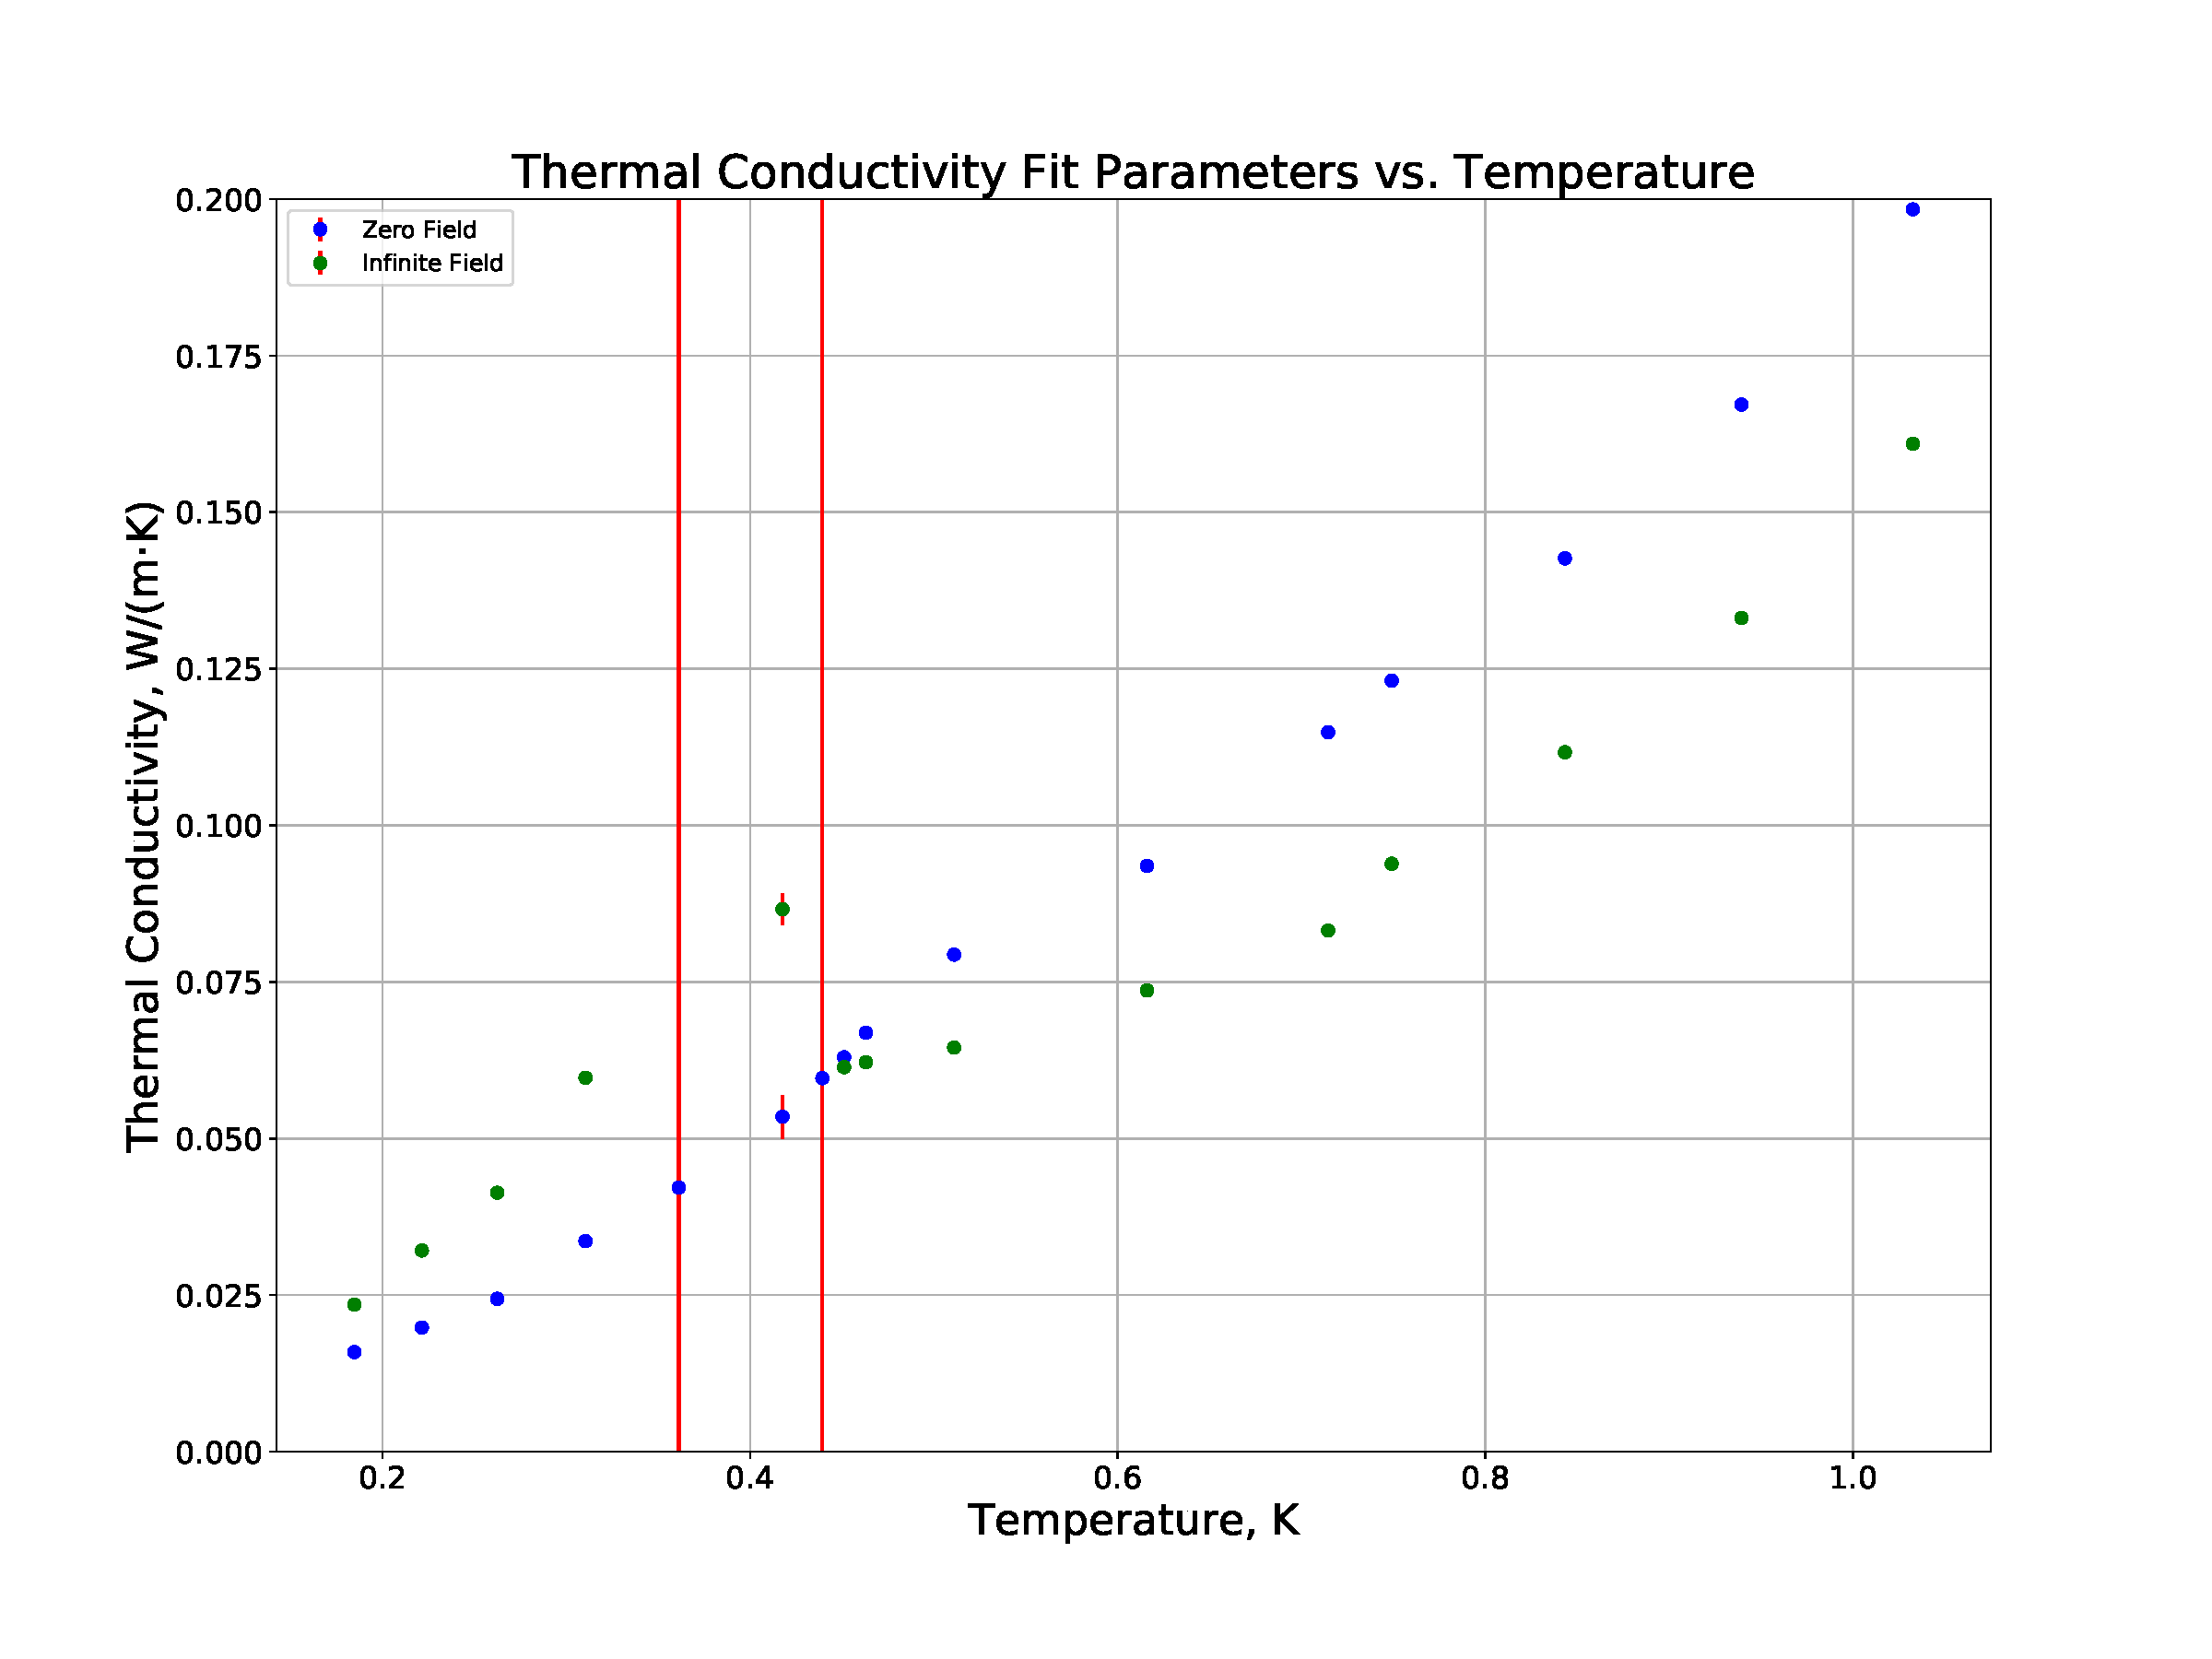
\includegraphics[width=0.9\columnwidth,trim={1cm 1cm 1cm 1cm},clip]{figures/SCBO_tcond_params.pdf}
\end{figure}

One other curious feature is the appearance of a very small thermal Hall conductivity at around 500 mK, shown in figure \ref{fig:SCBO_small_thall}. This only occurs at this specific temperature, and it is barely visible with the sensitivity of the Cernox thermometers. At the field with the strongest $\kappa_{xy}$, the thermal Hall angle is about $\tan \theta_H = 0.013$, which is relatively large compared to the other spin systems listed in table \ref{tab:hall_angles}. This is just above the temperature where the field dependence of the thermal conductivity flips over. Clearly, it is not like the thermal Hall signal predicted to arise as a result of the Chern bands, as it does not get stronger with higher temperature. It is hard to imagine this thermal Hall conducitivty coming from the triplons directly, since they should be frozen out at this temperature. Instead, it appears to be specific to crossover. 

\begin{figure}
	\centering
	\caption[Small thermal Hall conductivity in SCBO]{A very small thermal Hall conductivity, barely above the noise level, observed at a temperature of about 500 mK. This is just above the crossover temperature.}
	\label{fig:SCBO_small_thall}
	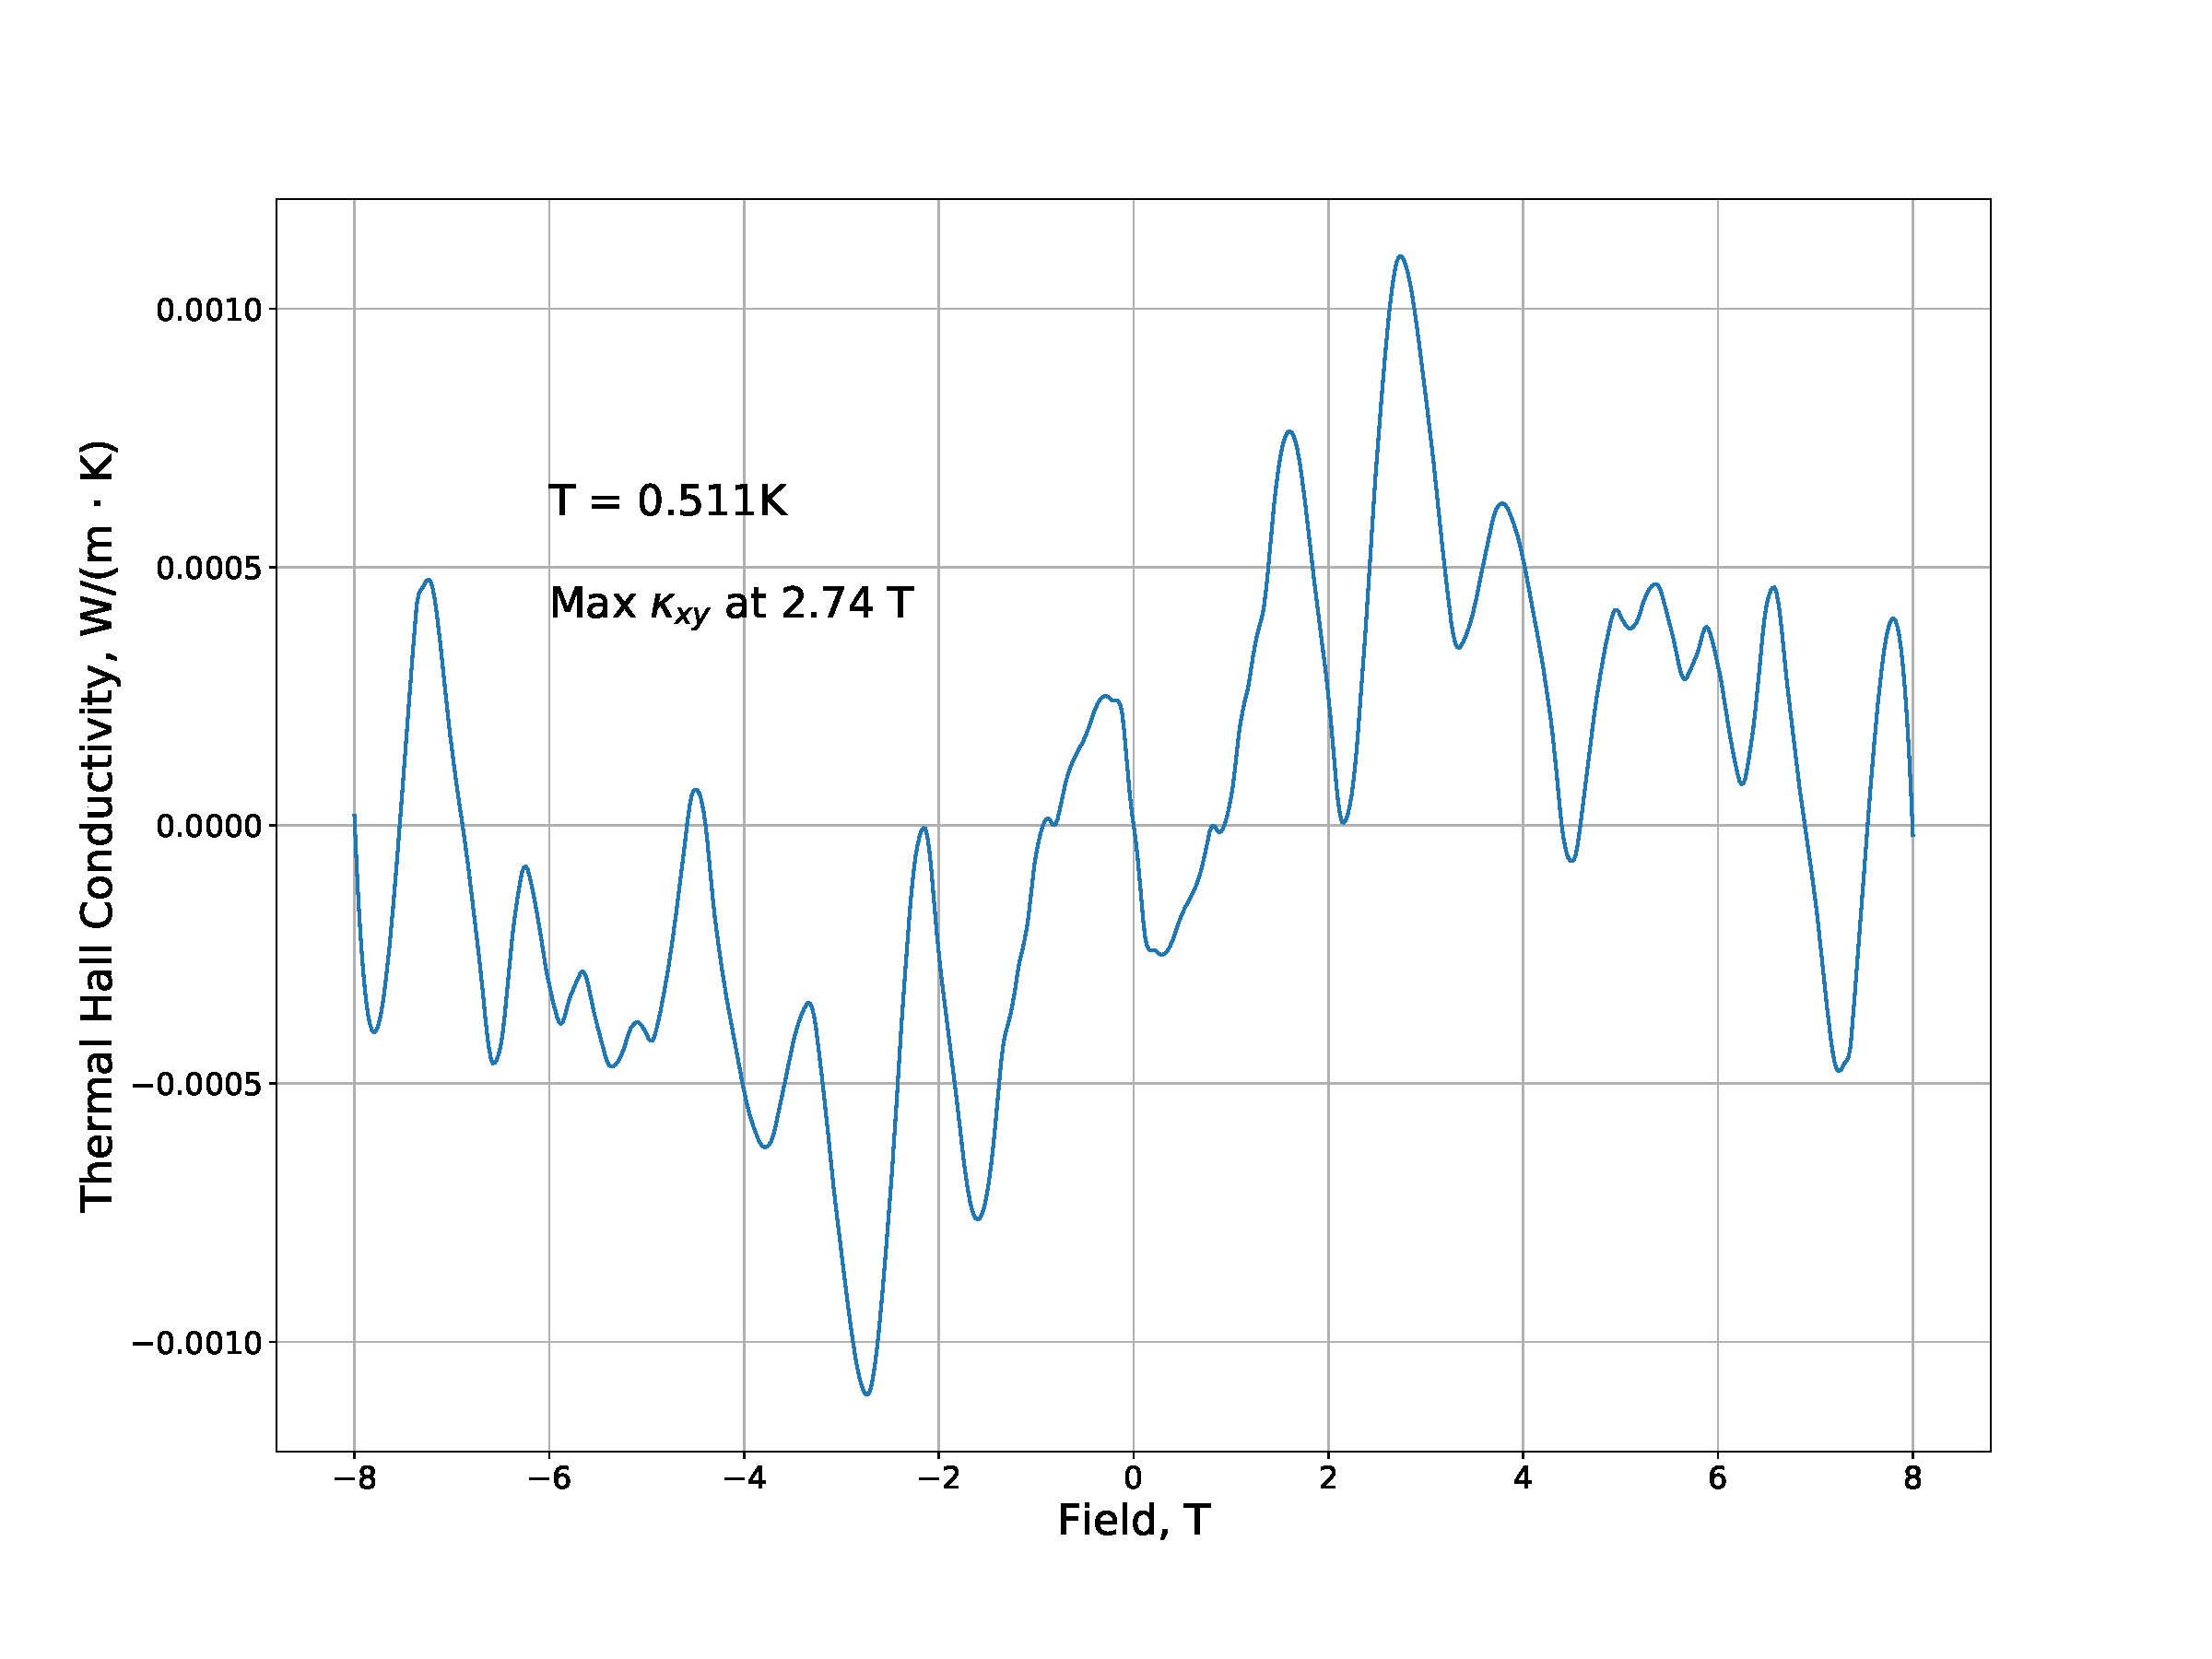
\includegraphics[width=\columnwidth]{figures/SCBO_kappa_xy_vs_B.pdf}
\end{figure}

One potentially interesting question to consider is how this thermal conductivity signal might be connected to another phenomena observed in SCBO at temperatures below 1 K: the formation of spin superlattices. When large magnetic fields are applied to SCBO, the energy of the triplet states with $s^z$ aligned with the applied field can be lowered to the point that they become populated, and arrange themselves into a lattice structure which is some multiple of the base lattice, hence the name ``superlattice''. The superlattices are labeled by what fraction of the total possible magnetization they have. Figure \ref{fig:SCBO_superlattice} shows the structure of the 1/8 superlattice, as well as it's experiemental signature in magnetic susceptibilty measurements at 22T~\cite{Haravifard2016}. In higher fields, experiments measuring magnetostriction~\cite{Jaime2012} and magnetization~\cite{Matsuda2013} has found evidence for 2/15, 1/4, 1/3, 2/5, and 1/2 superlattices. All of these occur at magnetic fields much higher than what we have measured, but all require temperature below 1 K. However, when a pressure of 2.2 GPa is applied to the crystal, a new superlattice attributed to a 1/20 superlattice occurs just above 5 T. This is within the range of the thermal conductivity experiements described above, and corresponds to the field scale we observed using the ansatz fits. Clearly the 1/20 superlattice is not forming in our experiments, which were conducted in vacuum. However, we can speculate that the field dependent thermal conductivity is related somehow to this ordering, or perhaps to whatever is supressing it at ambient pressure. The fact that the specific field dependence of $\kappa_{xx}$ changes with temperature may be a sign that there are competing phases involved, perhaps other, larger superlattices. Unfortunately, it appears more measurements will need to be conducted in order to say for sure if this is the case. 

\begin{figure}
	\centering
	\caption[Spin Superlattices in SCBO]{Spin Superlattices in SCBO. Top: Schematic of the 1/8 superlatticeobserved in SCBO at ambient pressure, reproduced from~\cite{Rice2002}. The lattice has one eighth of the total possible magnetization, with an arrangment which enlarges the unit cell of the layer, hence the term ``superlattice''. Bottom: experiemental signature of the formation of superlattices in SCBO from magnetic susceptilibty measurements, reproduced from~\cite{Haravifard2016}. A background has been subtracted to highlight the superlattice feature. Panel a shows measurments taken at ambient pressure. The 1/8 superlattice is formed at around 22 T. Panel b shows measurements taken at 2.2 GPa. In this case, a new superlattice forms above 5 T. In both cases, the superlattices only become clearly defined below 1 K.}
	\label{fig:SCBO_superlattice}
	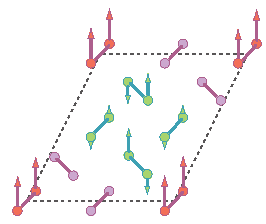
\includegraphics[width=0.6\columnwidth]{figures/SCBO_superlattice.pdf}
	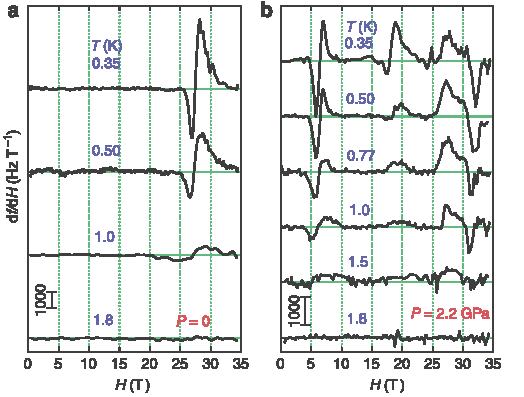
\includegraphics[width=0.9\columnwidth]{figures/SCBO_plateaus.pdf}
\end{figure}

\chapter{Conclusion}

Thermal measurements are an important tool for studying new materials and identifying novel physics in condensed matter systems. In a sense, they are the most general experimental methods available to a condensed matter experimentalist: any excitation in a solid will carry energy, and thus heat. This makes them particularly applicable to studying systems with novel excitations that do not carry charge. Such measurements can be quite challenging to make, however. They require accurate and precise readings of the temperature at multiple points on a crystal, which are often quite small, only a few millimeters in any direction. These thermometers must be compatible with the cryogenic environment where the measurement takes place, and may also need to be compatible with intense magnetic fields.

This is especially important when making thermal Hall effect measurements, the thermal analogue of the Hall effect. This effect is often minute, rarely more than 1\% of the total thermal conductivity. It also often requires making measurements in magnetic fields of a few Tesla or more. These fields can interfere with standard methods of thermometry relying on resistive thermometers by way of their magnetoresistance. In order to eliminate the systematic issues with these devices, we have exploited the strongly temperature dependent dialectic permittivty of strontium titanate. This material is not itself a ferroelectric, but sits close to a quantum phase transition to a ferroelectric state. This causes its permittivity to increase rapidly until reaching a maximum a few Kelvin above absolute zero. By making small capacitors using this material as a dielectric, we can use this fact to measure temperature with great precision in a way that is not systematically affected by a magnetic field. This observation on its own opens up new possibilities for making thermal Hall effect measurements in strong magnetic fields, but since the permittivity saturates below a few Kelvin, the sensitivity of these devices rapidly degrades in this range. However, it has been noted that annealing strontium titanate in an oxygen-18 atmosphere can tune the properties of this material close to this quantum critical point, even making it ferroelectric if enough is incorporated. By moving strontium titanate close to this quantum phase transition without going over, the permittivity can be made to keep increasing down to temperatures below 1 Kelvin, where the mangetoresistance issues of conventional thermometers are most severe. 

In order to test these capacitive thermometers, thermal Hall effect measurements were carried out on single crystalline bismuth. Bismuth is one of the best known semimetals, a material which hosts both electrons and holes, with a relatively low carrier density but high mobility. It is also well known for having ``Dirac-like'' bands, with carriers that have linear dispersion similar to a relativistic particle. These properties make it an important system for benchmarking new experimental techniques in condensed matter physics. Despite being an ``old material'', one which has been studied experimentally for over a century, thermal Hall effect measurements had only recently been performed on it up to 3 T. With the strontium titante microthermometers, we were able to conduct measurements up to 10 T and at temperatures down to 40 K. A large thermal Hall coefficient is measured in this system, indicative of high mobility carriers. Additionally, the overall field dependence displays a 1/$H$ dropoff far below the quantum limit, which can be traced to the presence of both electrons and holes. The strontium titanate microthermometers allow us to continue to observe these properties in the intense magnetic field.

Another important application of these thermometry techniques is towards making measurements of frustrated magnets. These are systems where the geometry of the lattice interferes with magnetic ordering, resulting in a variety of new magnetic phases such as spin ices and quantum spin liquids. These systems have generated quite a bit of theoretical interest in the past decade, but they are difficult to study experimentally since they often have itinerant excitations which do not carry charge. This makes thermal transport measurements such as the thermal Hall effect all the more important for studying them. In this work we discuss our measurements on strontium copper borate, in which pairs of spin-1/2 sites are paired up in dimers with a ground state made up of a lattice of singlets. The magnetic excitations of this system are the mobile triplet states, called triplons. It has been predicted that these triplet bands could have non-trivial topology, making strontium copper borate a bosonic topological insulator, and resulting in a specific thermal Hall effect signal. Experimental measurements in this system fail to find this signal, casting doubt on this theory. However, we observe magnetic field dependent longitudinal thermal conductivity at temperatures below 1 K, where the triplet excitations should be frozen out. There may be some relation to another phenomena found in this material in this temperature range: the formation of spin superlattices, states where spins form ordered arrangements larger than the base unit cell of the material.

Of course, the work presented here 

\appendix
\chapter{Python Source Code for Finite Element Simulations of the Thermal Hall Effect} \label{app:fem_src}

The following Python source code uses Fenics to do the finite element computations described in chapter 1. It will output the plots in the text as pdf files.

\begin{singlespace}
\begin{code}
from fenics import *
from mshr import *
import numpy as np
import matplotlib.pyplot as plt
import matplotlib

# Mesh
asp_ratio = 1.6
domain = Rectangle(Point(0.0, 0.0), Point(asp_ratio, 1.0))
mesh = generate_mesh(domain, 128)
V = FunctionSpace(mesh, 'P', 1)

# Dirichlet BC (Cold Finger)
u_D = Constant(0.0)

def boundary_D(x, on_boundary):
    return on_boundary and ((x[0] <= asp_ratio*x[1]) 
                       and (x[0] <= asp_ratio*(1-x[1])))

bc = DirichletBC(V, u_D, boundary_D)

# Neumann BC (Heater, Insulated Edges)
g = Expression('x[0] >= x[1]*{0} && x[0] >= (1-x[1])*{0} ? -1 : 0'
               .format(asp_ratio), degree=1)

thetas = np.pi*np.array([-1/6, -1/12, 0, 1/12,
                          1/6, 1/4, 1/3, 5/12])
xs = np.linspace(0,1.6,161)
ys = np.linspace(0,1.0,101)

us = np.zeros((thetas.size, xs.size, ys.size))

for ii, theta_hall in enumerate(thetas):

    # Thermal Hall Conductivity
    # C = as_matrix(((1, np.tan(theta_hall)),
    #                (-np.tan(theta_hall), 1)))
    C = as_matrix(((np.cos(theta_hall), np.sin(theta_hall)),
                   (-np.sin(theta_hall), np.cos(theta_hall))))

    # Weak Problem
    u = TrialFunction(V)
    v = TestFunction(V)

    a = dot(C*grad(u), grad(v))*dx
    L = -g*v*ds

    # Compute solution
    u = Function(V)
    solve(a == L, u, bc)

    us[ii] = np.array([[u(x, y) for x in xs] for y in ys]).T

font = {'size'   : 16}
matplotlib.rc('font', **font)

f, axarr = plt.subplots(4,2, sharex='col', 
                             sharey='row',
                             figsize=(9,12),
                             subplot_kw={'aspect':1})
theta_names = ['-$\\pi$/6', '-$\\pi$/12', '0', '$\\pi$/12',
               '$\\pi$/6', '$\\pi$/4','$\\pi$/3', '5$\\pi$/12']
levels = np.linspace(0, np.max(us), 24)
for theta, u, ax in zip(theta_names, us, axarr.flatten()):
    ax.contour(xs, ys, u.T, cmap='plasma', levels=levels)
    ax.set_title('$\\theta_H$ = {}'.format(theta))
    
f.savefig('thall_isotherm.pdf')

font = {'size'   : 14}
matplotlib.rc('font', **font)

f, (ax1, ax2) = plt.subplots(2, 1, figsize=(9,12))

for theta, u in zip(theta_names, us):
    diff = u[:,-1] - u[:,0]
    ax1.plot(xs, diff, label=theta)

ax1.set_title('Temperature Difference Profile')
ax1.set_xlabel('$x$, arb. units')
ax1.set_ylabel('$\Delta T$, arb. units')
ax1.grid()
ax1.legend()

ax2.plot(thetas_full, us_full[:,-1,-1] - us_full[:,-1,0])

ax2.set_title('Transverse Temperature Difference')
ax2.set_xlabel('Thermal Hall Angle $\\theta_H$, radians')
ax2.set_ylabel('$\Delta T$, arb. units')
ax2.grid()

f.savefig('thall_profile.pdf')

\end{code}
\end{singlespace}

\chapter{Operation of the Denton Evaporator}

\bibliography{./refs.bib}
\bibliographystyle{unsrt}

\end{document}
